\setchapterstyle{kao}
\setchapterpreamble[u]{\margintoc}


\chapter{Event Processing and Reconstruction}
\labch{simulation_and_processing}

The analysis presented in this thesis is highly dependent on an efficient filtering and event selection to reduce the raw IceCube trigger data to a usable atmospheric neutrino sample. Based on this selection, a precise estimation of both expected SM background and expected BSM signal events can be made using MC simulations. Starting from the PMT output, both data and simulation are processed through the in-ice trigger, the online filter and processing, and the low-energy event selection to produce a neutrino dominated sample. Once the sample is small enough for more sophisticated reconstruction techniques to be feasible to run, the events can be reconstructed with the existing IceCube reconstruction algorithms. At this level it is also possible to test and develop new reconstruction algorithms, without complications due to the large amount of background events from atmospheric muons and noise that are present before the filtering.

After describing the processing and filtering chain in \refsec{processing_chain}, the development and performance of a dedicated low-energy double-cascade reconstruction algorithm is presented in \refsec{dc_reconstruction}. Based on the results from this reconstruction, the ability of the detector to observe and identify double-cascades is discussed in \refsec{dc_classification}. Finally, the state-of-the-art IceCube low-energy event reconstruction is presented in \refsec{reconstruction}, which is used to perform the analysis in this thesis.


\section{Processing} \labsec{processing_chain}

After the detector simulation is performed, all MC and data are processed in exactly the same way. This section explains the trigger and event selection that is applied starting from the raw voltage measured by the PMTs. It is split in different steps that are run inside the ice, at the South Pole, and after the data was transferred to the North\sidenote{Since the IceCube detector is at the South Pole, the data storage and processing sites in the Northern Hemisphere are shortly referred to as \textit{the North}.}. The complexity and computational cost of the processing increases with each step, while the total number of events reduces, making it feasible and reducing the use of computational resources on events that are not of interest for analyses. 


\subsection{Trigger and Filter} \labsec{trigger_and_filter}

Before the data can be sent to the North, the initial signal coming from the PMT is a voltage waveform that is digitized (for data) and then information of photon hits are extracted (also for the MC coming from the detector response simulation). The trigger and filter explained here are tailored to select events that pass through the DeepCore volume, while rejecting background events (either from atmospheric muons or from random noise). There are other filters used in IceCube which will not be explained here, since they are not relevant for this work. A full description of the instrumentation and the online systems can be found in~\sidecite{Aartsen:2016nxy}.


\subsubsection{In-ice Trigger} \labsec{trigger}

The trigger is applied inside the DOM in the ice before sending the information to the ICL on the surface. The time dependent voltage curves are captured if a pre-defined threshold value is exceeded. Once the threshold, set to the equivalent of \SI{0.25}{PE}, is crossed, \SI{6.4}{\micro\second} of the waveform are coarsely digitized by a \textit{Fast Analog-to-Digital Converter (FADC)} with a sampling rate of \SI{40}{\mega\hertz}. Additionally, the first \SI{427}{\nano\second} are digitized using an \textit{Analog Transient Waveform Recorder (ATWD)} with a sampling rate of \SI{300}{\mega\hertz}~\sidecite{ABBASI2009294_data_acquisition}, but only if some trigger condition is met, because this readout frequency is too high to be sampled directly and requires some buffering. For DeepCore, the HLC condition already mentioned in \refsec{ice_and_DOMs} has to be met for three DOMs inside the fiducial volume within a time window of \SI{5}{\micro\second}. If this is the case, all waveforms that crossed the threshold within a \SI{20}{\micro\second} time window around the trigger are digitized and sent to the ICL for further processing. This trigger is called DeepCore \textit{Simple Multiplicity Trigger 3 (SMT-3)}. The DOM hits that are read out in this process, but do not meet the HLC condition, are called \textit{soft local coincidence (SLC)} hits. The rate of the DeepCore SMT-3 trigger is $\sim$\SI{250}{\hertz}~\cite{2017JInst..12P3012A_Instrumentation_Systems}.


\subsubsection{Online Filter} \labsec{online_filter}

The digitized waveforms are sent to the ICL, where a further filter is applied \textit{online}\sidenote{Where \textit{online} means running on hardware at the South Pole as opposed to \textit{offline} at the IceCube institutions in the Northern Hemisphere.}. First, the WaveDeform algorithm is run to extract photon arrival times and charge from the waveforms. Next, the DeepCore filter is applied, which is an iterative hit cleaning starting from HLC hits and removing any hits outside a \SI{125}{\meter} radius and a \SI{500}{\nano\second} time window (called \textit{radius-time cleaning (RT-cleaning)}) of the initial hit. This mainly rejects unphysical SLC hits, which are potentially caused by random noise. All following selection steps are done using the resulting cleaned pulses.

An additional cut is applied to reject events that are likely to be caused by atmospheric muons. This is done by splitting the hits depending on whether they were inside the DeepCore fiducial volume or outside and then calculating the speed of each hit outside the fiducial volume towards the \textit{center of gravity (COG)} of the hits inside. If one of them has a speed close to the speed of light, the whole event is rejected, because this is a strong indication for a muon event.

As input for the further selection levels, several event properties, such as vertex position and direction, are determined using fast and simple event reconstructions. After the DeepCore online filter is applied, the data rate is about \SI{15}{\hertz}, which can be sent to the North via satellite for further processing.


\subsection{Event Selection} \labsec{event_selection}

After the data was sent to the North, the \textit{offline} filters and selections are applied to further reduce the background of atmospheric muons and noise. The selection is split into three levels referred to as \textit{Level 3-5 (L3-L5)}, which bring down the muon rate to $\sim$\SI{1}{\milli\hertz}, while the remaining fraction of random noise is below \SI{1}{\percent}. The neutrino rate after this level is \SI{2}{\milli\hertz}, making it a neutrino dominated sample. Assuming a HNL mass of \SI{0.6}{\gev} and a mixing of 0.1, the expected rate of HNL events after the selection is $\sim$\SI{5}{\micro\hertz}. A more detailed investigation of the HNL selection efficiency is presented in \refsec{dc_reconstruction_performance}.


\subsubsection{Level 3} \labsec{level_3}

At the first offline filtering level, Level 3, one-dimensional thresholds are used to reduce atmospheric muons, pure noise, and coincident muons. This selection is targeting regions where the data/MC agreement is poor, so that more sophisticated \textit{machine learning (ML)} techniques can be applied at later levels. The selection is made using 12 control variables, that are inexpensive to compute for the very large sample at this stage. The variables are related to position, time, and overall number of hits in the event.

Pure noise hits, that are temporally uncorrelated, are cleaned by applying a \SI{300}{\nano\second} sliding window, requiring the containment of more than 2 hits at its maximum. Additionally, an algorithm is run to check whether the hits show some directionality, accepting them only if they do.

To reduce the amount of muons a series of thresholds is applied using spatial and temporal information. Events that have more than 9 hits observed above \SI{-200}{\meter} or the first HLC hit above \SI{-120}{\meter} are rejected as well as events where the fraction of hits in the first \SI{600}{\nano\second} of the event is above 0.37, ignoring the first two hit DOMs. Additionally, the ratio between hits in the veto region and the DeepCore fiducial volume is required to be below 1.5.

If a muon enters the detector after the data acquisition was already triggered, it causes events that span over a much larger time range. To reduce those coincident events, the time difference between first and last pulse cannot be above \SI{5000}{\nano\second}. This cut mainly affects a region of very poor data to MC agreement, because coincident events are not simulated at all.

The L3 selection removes \SI{95}{\percent} of the atmospheric muons and >\SI{99}{\percent} of pure noise hits, while keeping >\SI{60}{\percent} of the neutrino events. The sample now roughly contains muons/neutrinos/noise at a ratio of 100:10:1 with a total rate of $\sim$\SI{0.5}{\hertz}.


\subsubsection{Level 4} \labsec{level_4}

After the total rate was reduced by the simple selection criteria at L3 and the overall agreement between data and MC is established, ML techniques can be applied to further reduce the background. For Level 4, two \textit{Boosted Decision Trees (BDTs)}~\sidecite{BDT} classifiers are trained to separate neutrino events from atmospheric muons and noise hits, separately. The output of each classifier, a probability score, can be seen in \reffig{level_4_classifiers}. The noise filter is applied first and an event passes, if the score is larger than 0.7, reducing the noise hits by a factor of 100, while keeping \SI{96}{\percent} of neutrinos. Then the second BDT classifier is applied to reject muons. It was trained partly on unfiltered data, which consists of >\SI{99}{\percent} atmospheric muons, to reject the data and keeping the neutrinos from the simulation. Rejecting events with a score smaller than 0.65 removes \SI{94}{\percent} of atmospheric muons while keeping \SI{87}{\percent} of neutrinos. After applying the L4 selection, based on the BDT classifier outputs, the sample is still dominated by atmospheric muons, while the noise rate dropped to below most neutrino types.

\begin{figure*}
\centering 
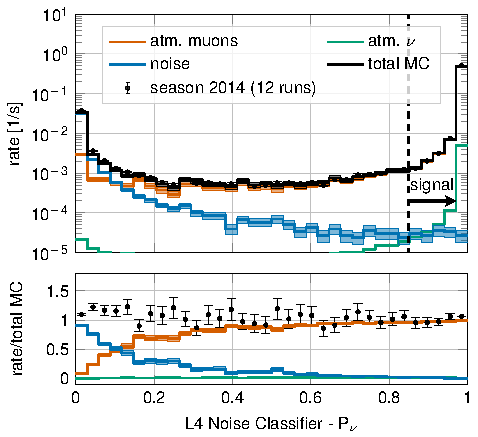
\includegraphics[width=0.49\linewidth]{figures/simulation_and_processing/selection/l4_noise_classifier_probnu.pdf}
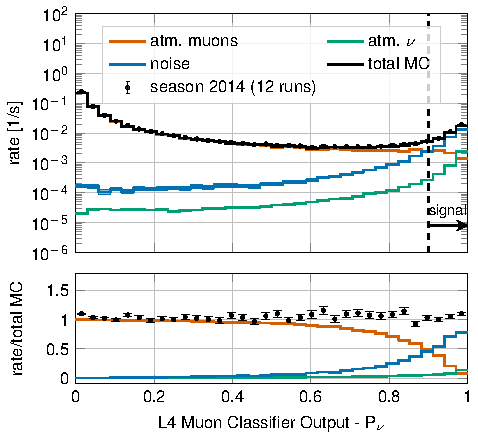
\includegraphics[width=0.49\linewidth]{figures/simulation_and_processing/selection/l4_muon_classifier_probnu.pdf}

\caption[Level 4 classifier outputs (muon and noise)]{Distributions of Level 4 noise classifier output (left) and muon classifier output (right), where larger values indicate more neutrino-like and lower values more noise-like/muon-like. Taken from~\cite{OVS_PRD}.}
\labfig{level_4_classifiers}
\end{figure*}


\subsubsection{Level 5} \labsec{level_5}

Level 5 is the final selection level, before event reconstructions are applied. This level aims to reduce the remaining atmospheric muon rate below the rate of neutrinos. Muons not rejected by the earlier levels are those that produced little or no light in the veto regions. One possible reason is that they passed through one of the uninstrumented regions between the strings called \textit{corridors}. To reject those, special corridor selection criteria are applied, which are based on the number of hits the event produced close to a potential corridor it passed through. The potential corridor in questions is identified based on a simple infinite track fit. In addition to the corridor selection, starting containment conditions are applied to reject events that start at the edge of the fiducial volume. Events with more than seven hits in the outermost strings of the detector or those that have a down-going direction in the uppermost region are rejected. This further reduces the fraction of muons by \SI{96}{\percent} while keeping \SI{48}{\percent} of neutrinos.


\section{Double-Cascade Reconstruction} \labsec{dc_reconstruction}

In the energy range relevant for this work, around 10s of \si{\gev}, the light deposition is very low and only a few DOMs detect photons, making event reconstructions difficult. Existing reconstruction algorithms applied for low-energy atmospheric neutrino events are either assuming a single-cascade hypothesis or a track and cascade hypothesis, which are the two SM morphologies observable at these energies, as was described in \refsec{icecube_signatures}. A HNL being produced and decaying inside the IceCube detector however, should produce two cascade-like light depositions. The morphology, spatial separation between the cascades, and their individual properties depend on the model parameters discussed in \refsec{double_cascade_morphology}. To investigate the performance of the detector to observe and identify these events, a low-energy double-cascade reconstruction algorithm was developed. It is based on a pre-existing algorithm used to search for double-cascades produced from high-energy astrophysical tau neutrinos~\sidecite{Abbasi:2020zmr} that was established in~\sidecite{PHallen, MUsner}.


\subsection{Table-Based Minimum Likelihood Algorithm}

The double-cascade reconstruction is relying on a minimum likelihood algorithm, which is the \textit{classical} approach to IceCube event reconstructions, as opposed to ML based methods. It compares the observed light depositions in the detector to the expected light depositions from a given event hypothesis, where the event hypothesis can be constructed from building blocks of single-cascade and track segment expectations. Varying the energies of the track segments and cascade components changes the light expectation and can be used to find the best fit hypothesis to the observed data. A Poissonian likelihood is constructed, which compares the observed photon numbers, $n$, with their arrival times to the expected light depositions, $\mu$, for a given event hypothesis as
\begin{equation}
    \ln(L) = \sum_j \sum_t n_{j,t} \cdot \ln(\mu_{j,t}(\Theta) + \rho_{j,t}) - (\mu_{j,t}(\Theta) + \rho_{j,t}) - \ln(n_{j,t}!)
    \;,
    \labeq{millipede_likelihood}
\end{equation}
where $\rho$ are the number of expected photons from noise, $\Theta$ are the parameters governing the source hypothesis, and the likelihood is calculated summing over all DOMs, $j$, splitting observed photons into time bins, $t$. The light expectations are calculated using look-up tables~\sidecite{photospline} that contain the results from MC simulations of cascade events or track segments. By varying the parameters defining the event hypothesis, the likelihood of describing the observed light pattern by the expected light depositions is minimized to find the reconstructed event. Algorithms of this kind, used in IceCube, are described in more detail in~\sidecite{IceCube:2013dkx}. For the table production a specific choice of ice model has to be made, while the calibrated DOM information is taken from the measurement itself.

Based on the tabulated light expectations for cascades and track segments, various hypotheses describing different event morphologies can be constructed. These are commonly the cascade only or the track and cascade hypotheses. The hypothesis describing the double-cascade signature of the HNL is using two cascades that are separated by a certain distance. The whole hypothesis is defined by 9 parameters and assumes that the two cascades are aligned with each other, which is a safe assumption for strongly forward boosted interactions and because low-energy cascades do not show a strong directionality. The parameters are the position of the first cascade, $x, y, z$, the direction of both cascades, $\phi, \theta$, and its time, $t$, as well as the decay length, $L$, between the two cascades. Assuming the speed of the HNL to be the speed of light, $c$, this already defines the full hypothesis, because the time and position of the second cascade are then fully determined by properties of the first cascade and the decay length. Note here, that the HNL particle does not produce any light while traveling, as it is electrically neutral. Since the likelihood only sums over DOMs that have observed photons, the non-observation of light is implicitly used as information and will exclude hypotheses with light expectation in those DOMs. The full 9 parameters describing an event are $\Theta = (x, y, z, t, \theta, \phi, E_0, E_1, L)$. To compute the full likelihood, the term in \refeq{millipede_likelihood}, defined for a single event hypothesis, is summed over both cascade contributions, as $\sum_i \ln(L_i)$, with $i$ being the cascade indices.


\subsection{Optimization for Low Energies}

Optimizing the double-cascade reconstruction for low-energy events was done in parallel to the development of the model-dependent simulation generator introduced in \refsec{model_specific_simulation}. A preliminary sample of HNL events from the model-dependent simulation was used, containing a continuum of masses between \SIrange[range-phrase=~and~]{0.1}{1.0}{\gev} and lab frame decay lengths sampled uniformly in the range from \SIrange{5}{500}{\meter}. Even though this sample is not representative of a physically correct model and therefore not useful to predict the event expectation, it can still be used to optimize the reconstruction. The double-cascade nature of the individual events is present and the evenly spaced decay length distribution is especially useful for the purpose of optimizing the reconstruction.

The simulation is processed up to Level 5 of the selection chain described in \refsec{event_selection} and the \textit{Retro} reconstruction from~\sidecite{low_energy_reco_IC} is applied to the events, fitting a cascade and a track and cascade hypothesis. The results from this reconstruction are used as an input for the double-cascade reconstruction, where the position of the vertex, the direction of the event, and its interaction time are used as the input quantities for the first cascade, and the length of the track reconstruction is used as a seed for the distance between the two cascades. Several reconstructions were tested as seeds for the vertex position and the direction, but the choice did not significantly alter the results reported here.


\subsubsection{Fit Routine}

\begin{marginfigure}
	\centering
    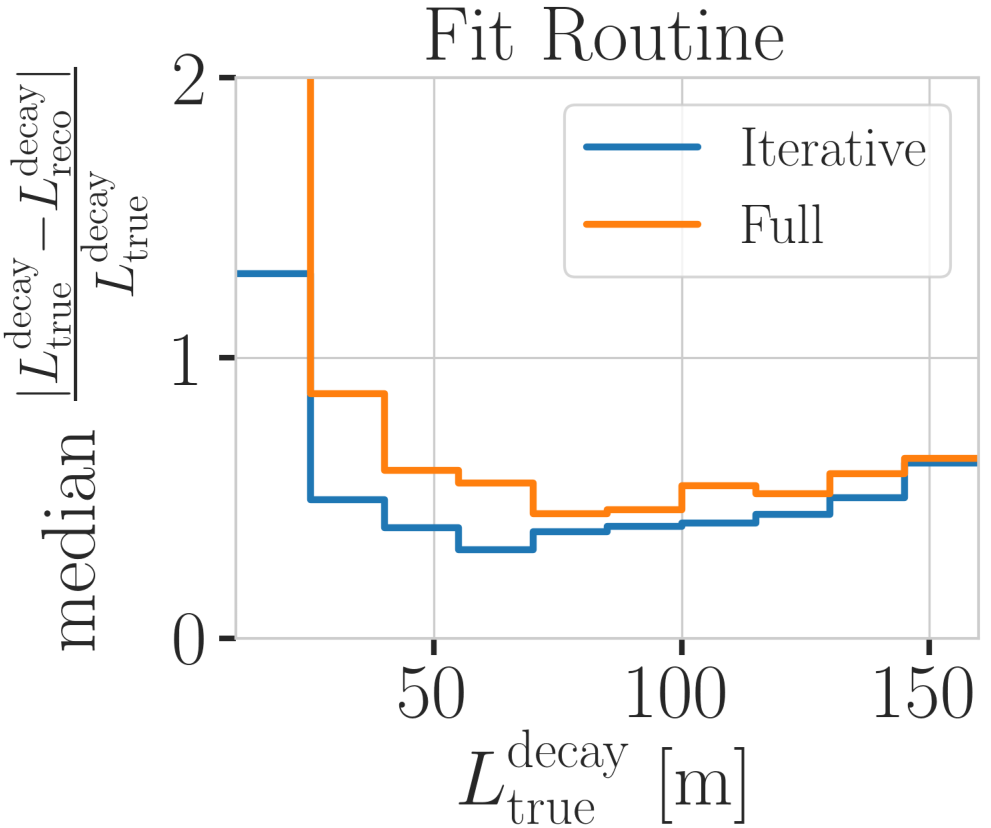
\includegraphics{figures/results/190605_reco_optimization/fit_routine_splitting_median_decay_length_resolution_Good + L7 + reco E1,E2 above 3_fix_y_new.png}
    \caption[Decay length resolution to optimize fit routine]{Decay length resolution as a function of the true decay length, comparing a full 9 parameters fit to an iterative approach where first the energies and the decay length are fit, while fixing the other 7 parameters and then the full fit is performed.}
    \labfig{fit_routine_optimization_fit_routine}
\end{marginfigure}

The full 9 dimensional likelihood space is very complex and can have many local minima, depending on the specific event and its location in the detector. For this reason, a more sophisticated fit routine than fitting all 9 parameters at once was tested. In a first fit iteration, some parameters are fixed and the resulting best fit point is used to fit all 9 parameters in a second iteration. The effect is shown in \reffig{fit_routine_optimization_fit_routine}, which shows the median of the absolute, fractional decay length error with respect to the true decay length, for the full fit and an iterative fit routine. It can be seen how a fit split into two consecutive steps, where the first step fits only both cascade energies and the decay length and the second step fits the full 9 parameters, performs better as compared to a single, full 9 parameter fit. The initial seed remains identical for both the routines.


\subsubsection{Decay Length Seeds}

\begin{marginfigure}
	\centering
    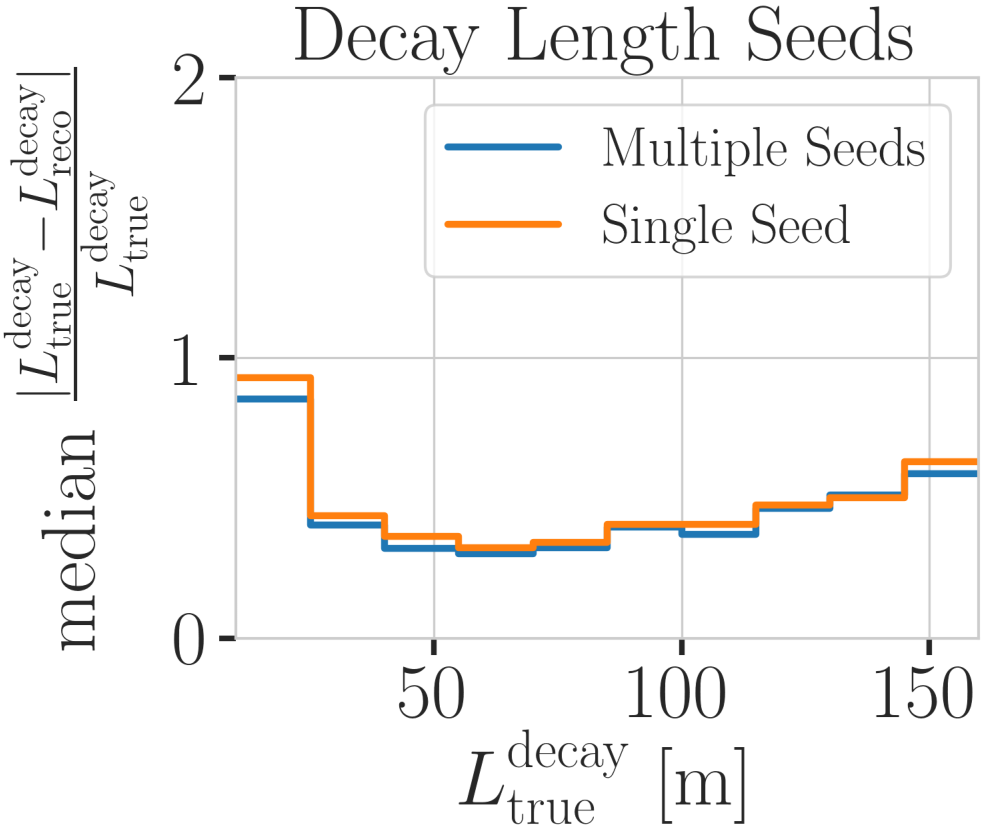
\includegraphics{figures/results/190605_reco_optimization/decay_length_seeding_median_decay_length_resolution_Good + L7 + reco E1,E2 above 3_fix_y_new.png}
    \caption[Decay length resolutions to optimize length seeding]{Decay length resolution as a function of the true decay length, comparing the same fit routine seeded with just the seed decay length and seeded with a decay length of \SI{5}{\meter}, \SI{25}{\meter}, \SI{50}{\meter}, \SI{100}{\meter}, and \SI{200}{\meter} on the left.}
    \labfig{fit_routine_optimization_decay_length_seeding}
\end{marginfigure}

From the seed values of the reconstruction, especially the length between the two cascades was found to have a very strong impact on whether the global minimum was found during the minimization. To mitigate this effect, multiple fits are performed, seeding with variations of the input length at different orders of magnitude. The best result is used, selected based on the total likelihood value of the best fit parameter set. A small improvement in the decay length resolution can be found by using this approach as compared to a single length seed. The resolutions for the differnt approaches are shown in \reffig{fit_routine_optimization_decay_length_seeding}.


\subsubsection{Minimizer Settings}

\begin{marginfigure}
	\centering
    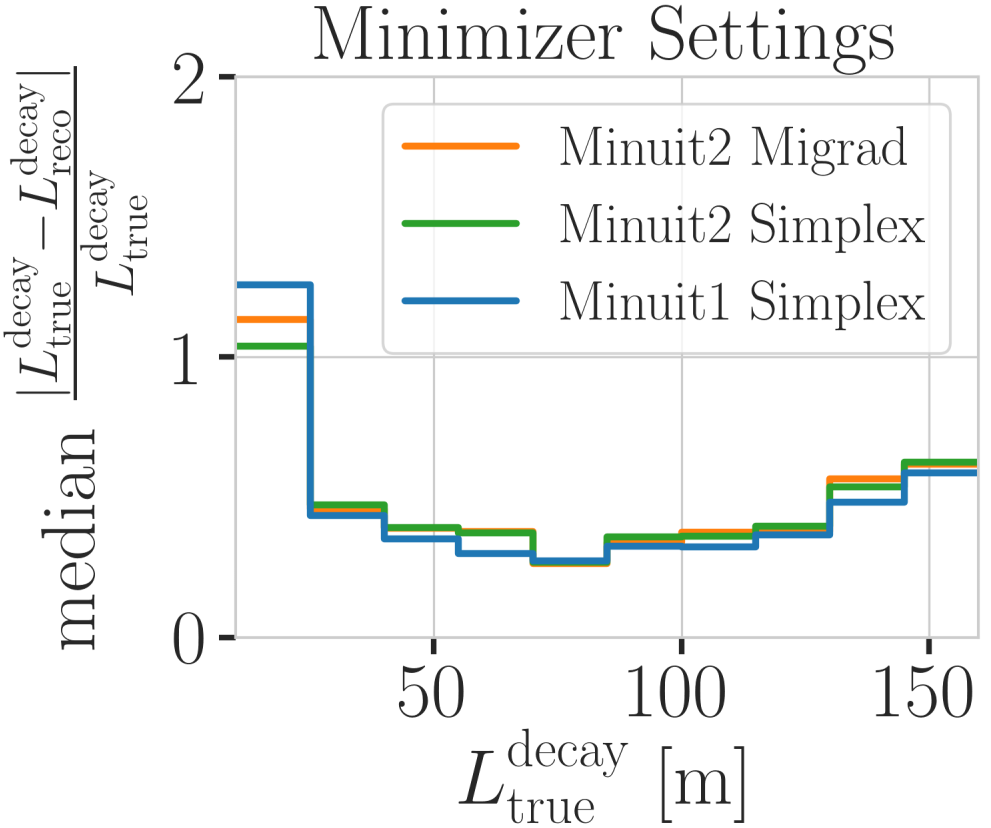
\includegraphics{figures/results/190605_reco_optimization/minimizer_checks_median_decay_length_resolution_Good + L7 + reco E1,E2 above 3_fix_y_new.png}
    \caption[Decay length resolution to optimize minimizer settings]{Decay length resolution as a function of the true decay length, comparing the same fit routine performed with different minimizers.}
    \labfig{fit_routine_optimization_minimizer_checks}
\end{marginfigure}

To investigate the effect of the minimizer used to find the best fit parameters, the reconstruction was performed using three different minimizers, which were easily accessible within the reconstruction framework. The minimizers used were Minuit1 Simplex, Minuit2 Simplex, and Minuit2 Migrad~\sidecite{og_minuit}. As can be seen in \reffig{fit_routine_optimization_minimizer_checks}, Minuit1 Simplex performed best and was chosen as the default for the reconstruction. Global minimizers may improve the performance of the reconstruction, but were not available in the framework and would require significant software development.


\subsection{Performance} \labsec{dc_reconstruction_performance}

The optimization of the reconstruction was performed using preliminary development versions of the model-dependent HNL simulation. To investigate the effect of the low-energy event selection and the double-cascade reconstruction performance in a generic way, the model-independent simulation introduced in \refsec{model_independent_simulation} is used. The important advantage of the model-independent samples is the controllable parameter space, especially in cascade energies and decay length, because the event kinematics are not coupled to the underlying HNL model, but can be chosen freely. This means that some benchmark edge cases can be investigated, and the performance can also be assessed for a realistic scenario in addition to mapping out the effects of the event selection and where the reconstruction breaks down.

\begin{margintable}
    \footnotesize
    \begin{tabular}{ ll }
    \hline\hline    
    \textbf{Type} & \textbf{Setting} \\
    \hline\hline
    Minimizer & Minuit1 Simplex \\
    $L_\rm{decay}$ seeds & $(0.5, 1.0, 1.5) \cdot L_\rm{seed}$ \\
    Fit routine & Iterative \\
    \hline
    \end{tabular}
\caption[Double-cascade reconstruction settings]{Chosen settings for the double-cascade reconstruction algorithm.}
\labtab{dc_reco_settings}
\end{margintable}

The chosen final settings and procedures used for the low-energy double-cascade reconstruction algorithm are summarized in \reftab{dc_reco_settings}. In the first fit iteration, the number of time bins in \refeq{millipede_likelihood} is set to 1, so just the number of photons and their spatial information is used. In the second step the number of time bins is chosen such that each photon falls into a separate time bin, which means all time information is used. The average runtime per event is $\sim$\SI{16}{\second} on a single CPU core, but is very dependent on the number of photons observed in the event, since the likelihood calculation in the second step scales with this number and a table lookup has to be performed for each photon.


\subsubsection{Best-Case Events}

\begin{marginfigure}
    \centering
    % [trim=left bottom right top, clip]
    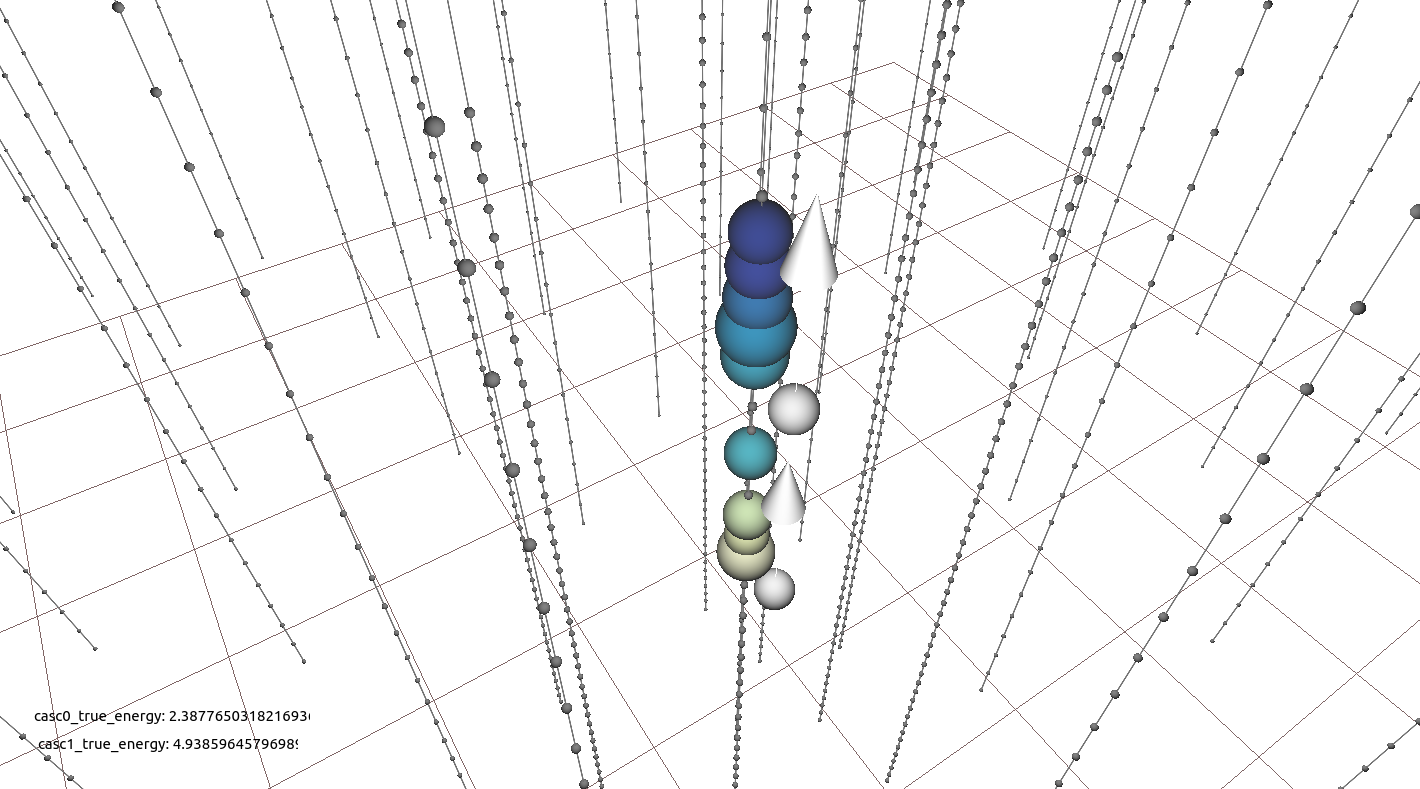
\includegraphics[trim=270 40 225 35, clip]{figures/model_independent_simulation/upgoing_e0_2.4_e1_4.9_v2.png}
    \caption[Event view of an up-going double-cascade event]{Event view of an up-going double-cascade event, with cascade energies of \SI{2.4}{\gev} and \SI{4.9}{\gev}, and a decay length of \SI{65.8}{\meter}. The colored spheres show the DOMs that have observed light, where the size is proportional to the number of observed photons and the color indicates the time (yellow is early, blue is late). The strings are shown as black lines, with small spheres indicating the DOM positions, and the true cascade vertices and directions are shown as white spheres with white arrows.}
    \labfig{up-going_example_event}
\end{marginfigure}

The best-case scenario to observe an event is to be directly on top of a string with a straight up-going direction. Using the simulation sample introduced in \refsec{simplistic_samples} and running the double-cascade reconstruction from \refsec{dc_reconstruction} on these events, it is possible to estimate the performance limit of the reconstruction. \reffig{up-going_example_event} shows one example event view from that sample, where the cascade energies are \SI{2.4}{\gev} and \SI{4.9}{\gev}, and the decay length is \SI{65.8}{\meter}. It can be seen that despite the low energies, both cascades deposit light in the DOMs and the reconstruction is expected to work.

\begin{figure*}[h]
	\centering
    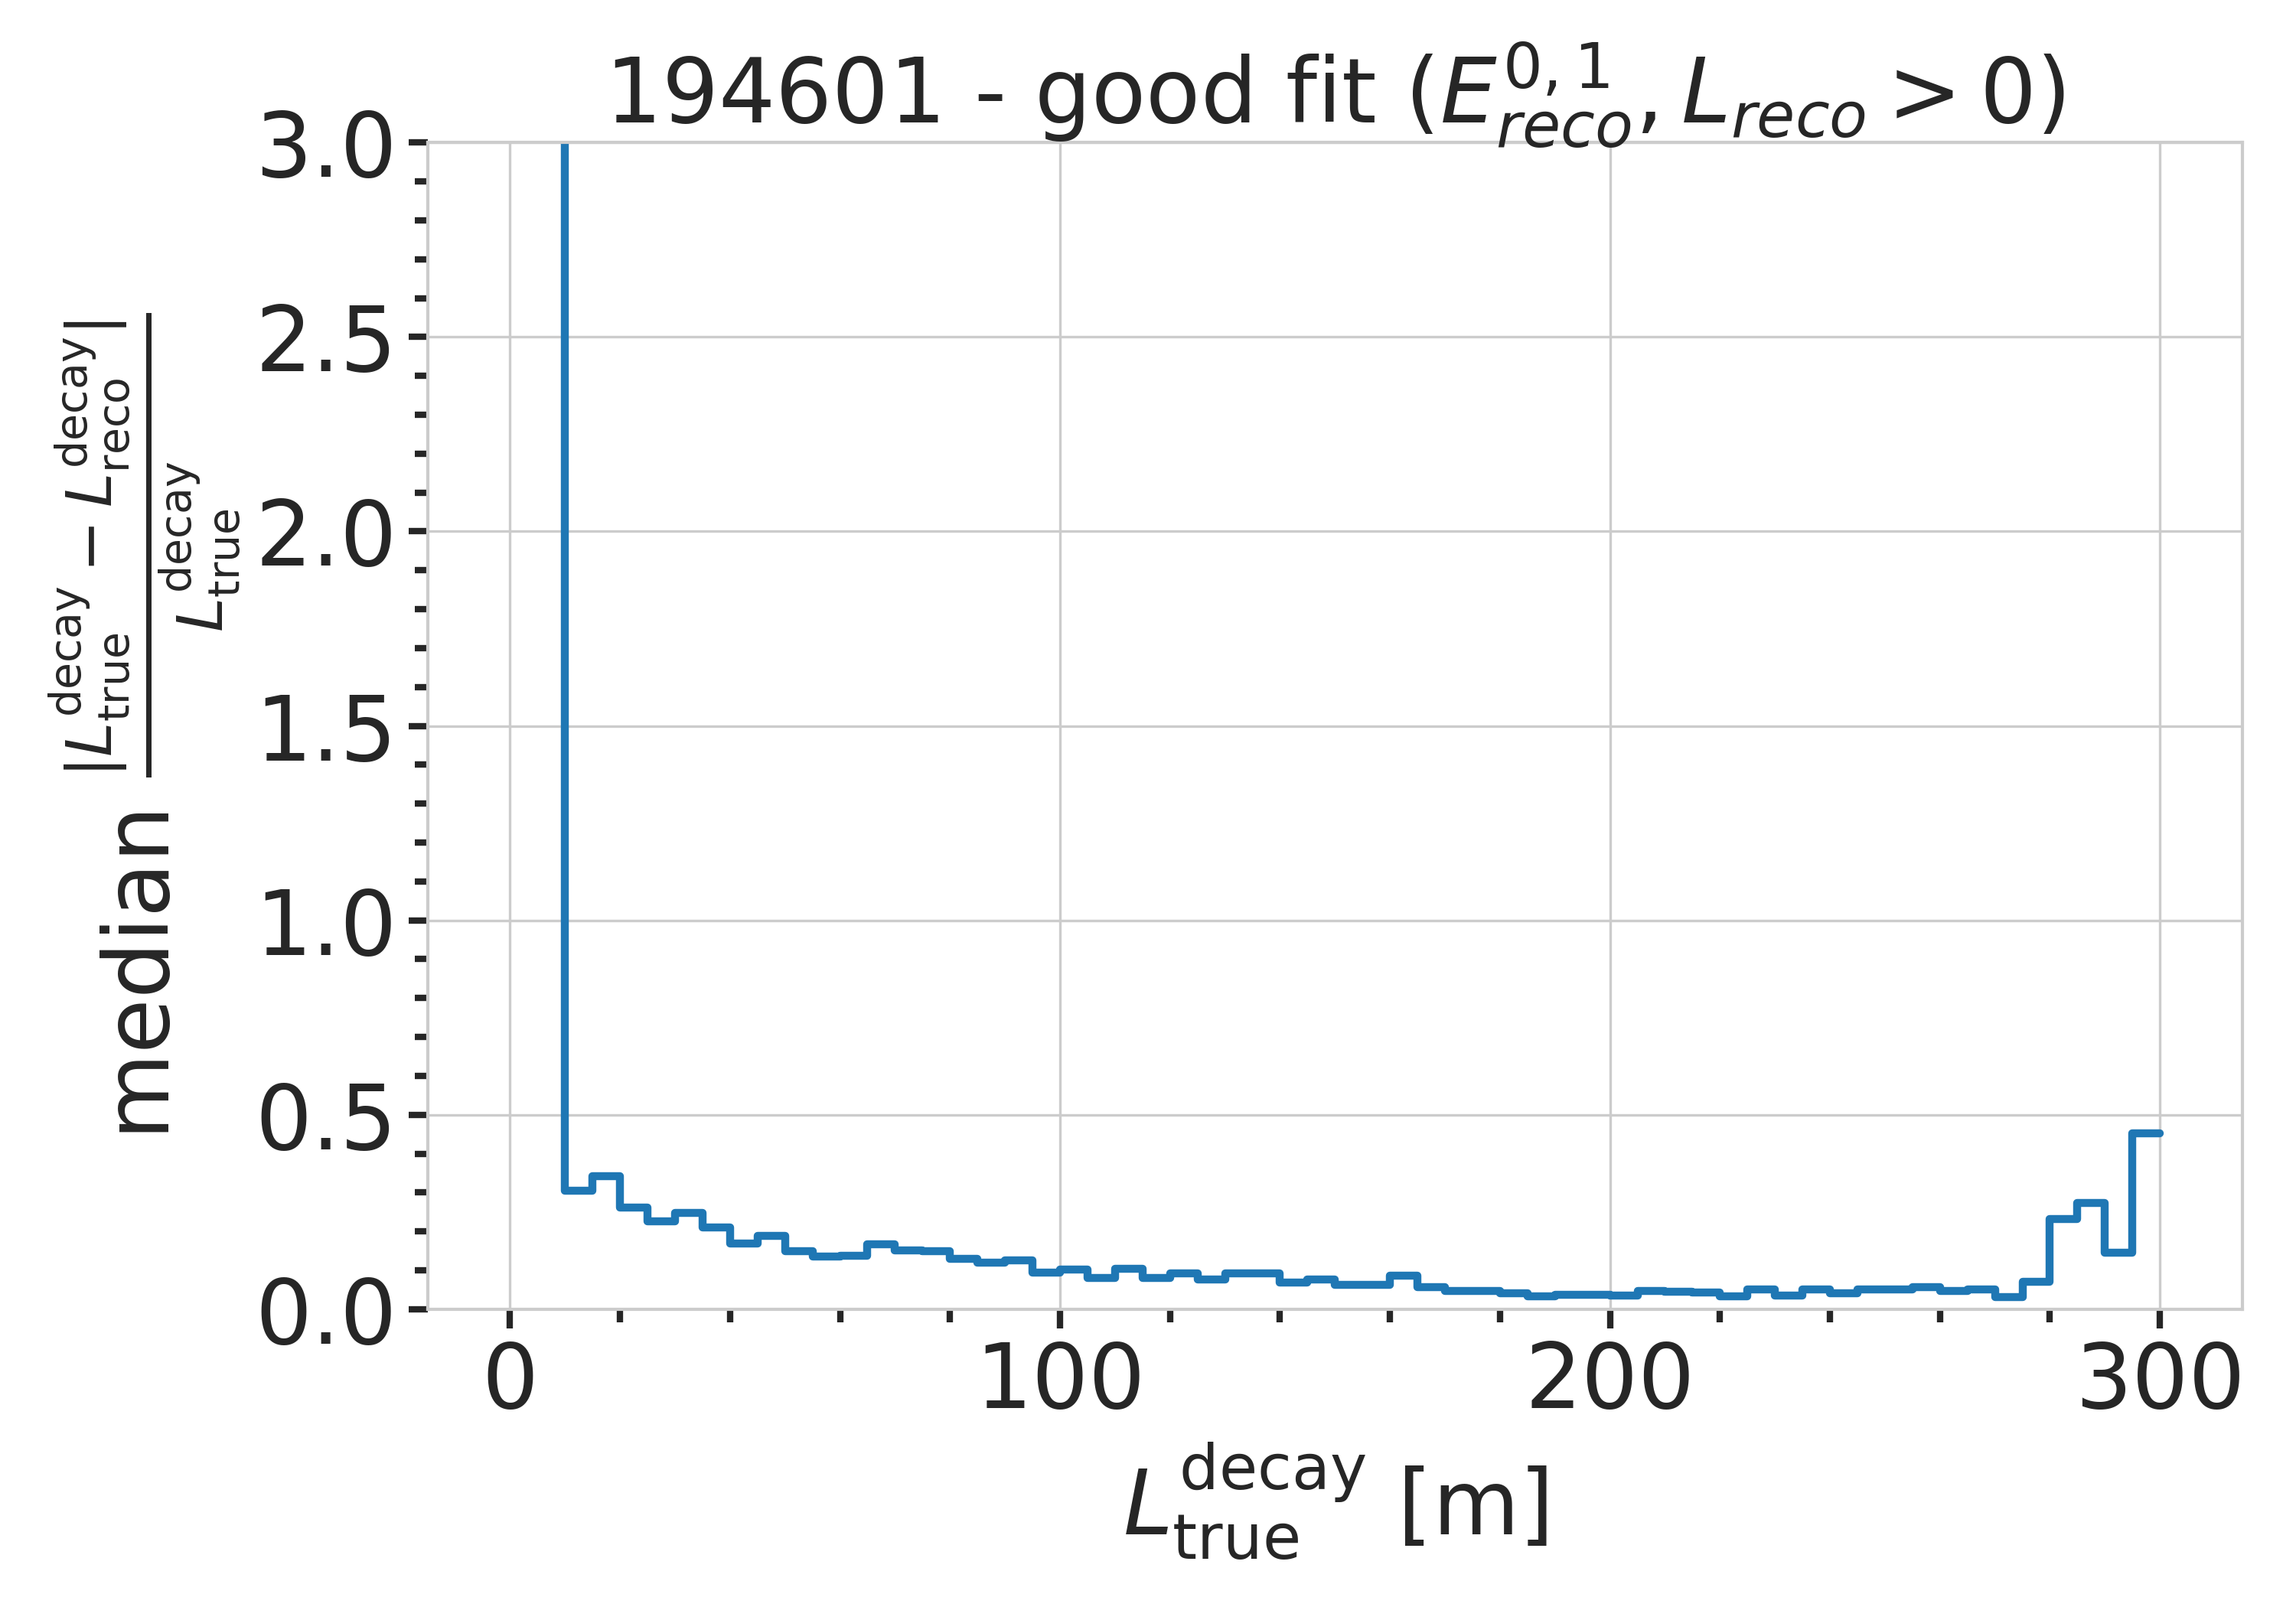
\includegraphics[width=0.47\linewidth]{figures/model_independent_simulation/results/idealistic/194601_median_decay_length_resolution_goodfit_log_unweighted.png}
    \includegraphics[width=0.51\linewidth]{figures/model_independent_simulation/results/idealistic/194601_reco_decay_length_vs_true_decay_length_goodfit_step_contours_new.png}
    \caption[Up-going double-cascade decay length resolution]{Decay length resolution of events from the up-going sample. Shown is the decay length resolution as a function of the true decay length (left) and the reconstructed decay length versus the true decay length (right), where the color scale is normalized per vertical slice and the median and \SI{68}{\percent} band are shown in red.}
    \labfig{idealistic_length_resolutions}
\end{figure*}

The length resolution for events from this sample is shown in \reffig{idealistic_length_resolutions}. In the left part, the median resolution is shown to be below \SI{30}{\percent} above a true decay length of $\sim$\SI{10}{\meter}, and decreasing with increasing true length, down to $\sim$\SI{10}{\percent} at \SI{100}{\meter}. In the right part of \reffig{idealistic_length_resolutions}, the reconstructed decay length versus the true decay length is shown. The color scale shows the PDF along each (vertical) true decay length slice, which additional information highlighted by the median and \SI{68}{\percent} band shown in red (also per vertical column). The two-dimensional histogram shows that there is no under-estimation of the length up to a true decay length of $\sim$\SI{210}{\meter}, which shows that if there are DOMs in the region between the two cascades that have not observed any light, the reconstruction is very stable. Considering the underlying Poisson likelihood in \refeq{millipede_likelihood} used for the reconstruction, this makes sense, since DOMs being present, but not observing any light is affecting the light expectation that goes into the likelihood and therefore makes these hypotheses incompatible with the data.


\subsubsection{Realistic Events}

The sample of HNL events introduced in \refsec{realistic_sample}, which is a more realistic representation of the expected HNL events, but still offers more controlled energy and length distributions, is used to investigate the selection efficiency, to cross-check the reconstruction performance, and to benchmark the limits where the reconstruction breaks down. An example event view is shown in \reffig{realistic_example_event}, for cascade energies of \SI{30.8}{\gev} and \SI{25.3}{\gev}, and a decay length of \SI{144.5}{\meter}. Since the size of the colored spheres is proportional to the number of photons observed in the DOMs, it can be seen from the event view that even for these higher energies, only individual or few photons are observed. This makes detecting and reconstructing them significantly more challenging and is purely due to the larger distance of the cascades from the DOMs.

\begin{marginfigure}
    \centering
    % [trim=left bottom right top, clip]
    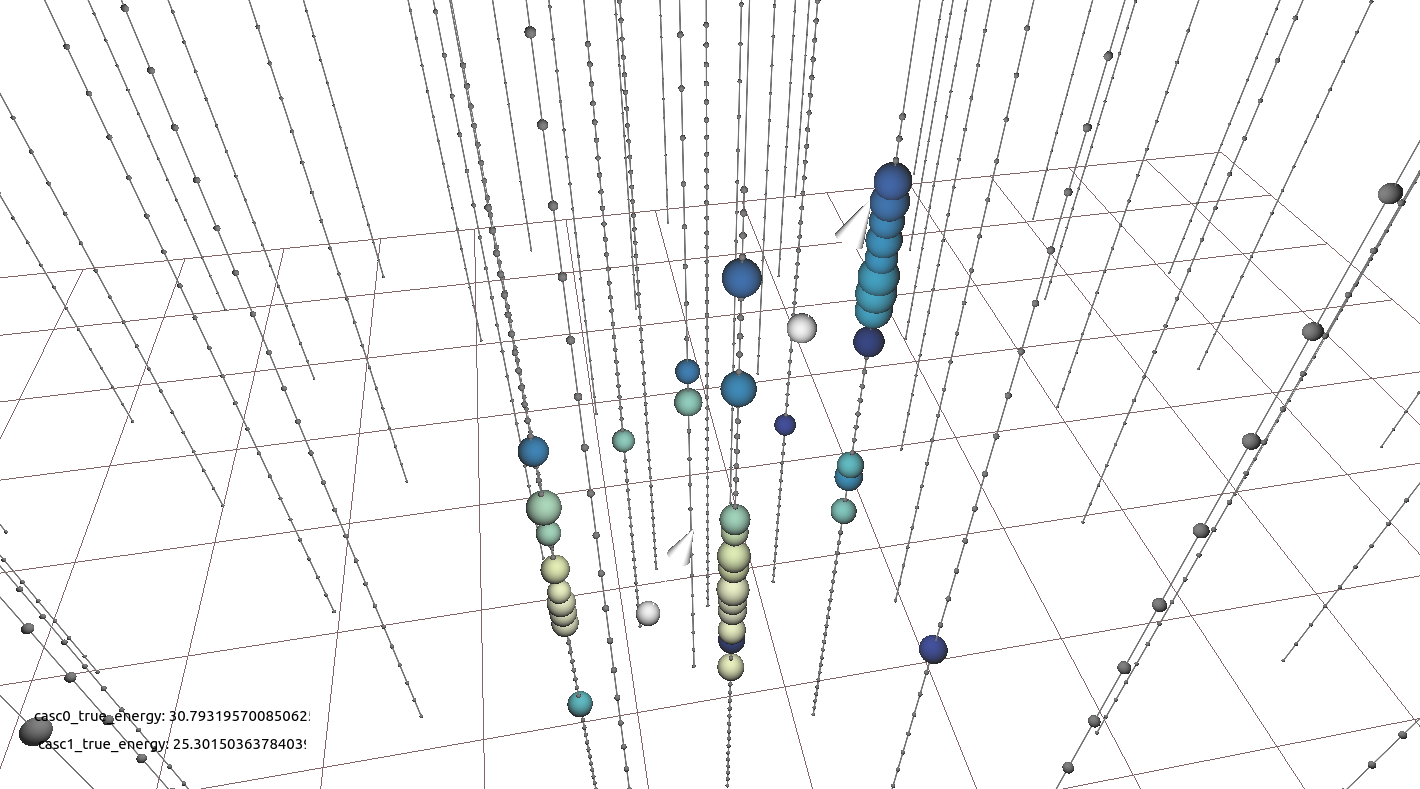
\includegraphics[trim=230 45 230 65, clip]{figures/model_independent_simulation/diagonal_e0_30.8_e1_25.3_v0.png}
    \caption[Event view of a realistic double-cascade event]{Event view of a realistic double-cascade event, with cascade energies of \SI{30.8}{\gev} and \SI{25.3}{\gev}, and a decay length of \SI{144.5}{\meter}. The colored spheres show the DOMs that have observed light, where the size is proportional to the number of observed photons and the color indicates the time (yellow is early, blue is late). The strings are shown as black lines, with small spheres indicating the DOM positions, and the true cascade vertices and directions are shown as white spheres with white arrows.}
    \labfig{realistic_example_event}
\end{marginfigure}


\paragraph{Energy Resolutions:}

The energy resolutions are inspected by looking at the two-dimensional distributions of reconstructed energy versus the true energy. The results for the energies of the individual cascades are shown in \reffig{cascade_energy_2dhists}, where the color scale is again normalized per vertical slice, and the median and \SI{68}{\percent} band are shown in red. For both cascades the reconstruction performs well above around \SIrange{5}{7}{\gev}, with the median being on top of the diagonal and the spread being small. Below this energy, the reconstruction is over-estimating the true energy. This is because, on average, those low-energy events, passing the event selection, interact closer to the DOMs and have an over fluctuation in their light deposition. This results in the observed energy bias. Interestingly, the second cascade energy reconstruction performs slightly worse, although they have the same energy ranges for this sample. This could hint at an asymmetry in the reconstruction process, which might be related to how the two cascades are parameterized, or be due to the different positions and the dominantly up-going direction used in the sampling combined with the DOMs looking down. Towards the higher energies, the statistics are decreasing, wich is due to the underlying energy distribution of the sample, which were shown in \reffig{realistic_gen_distris}.


\begin{figure*}[h]
    \centering
    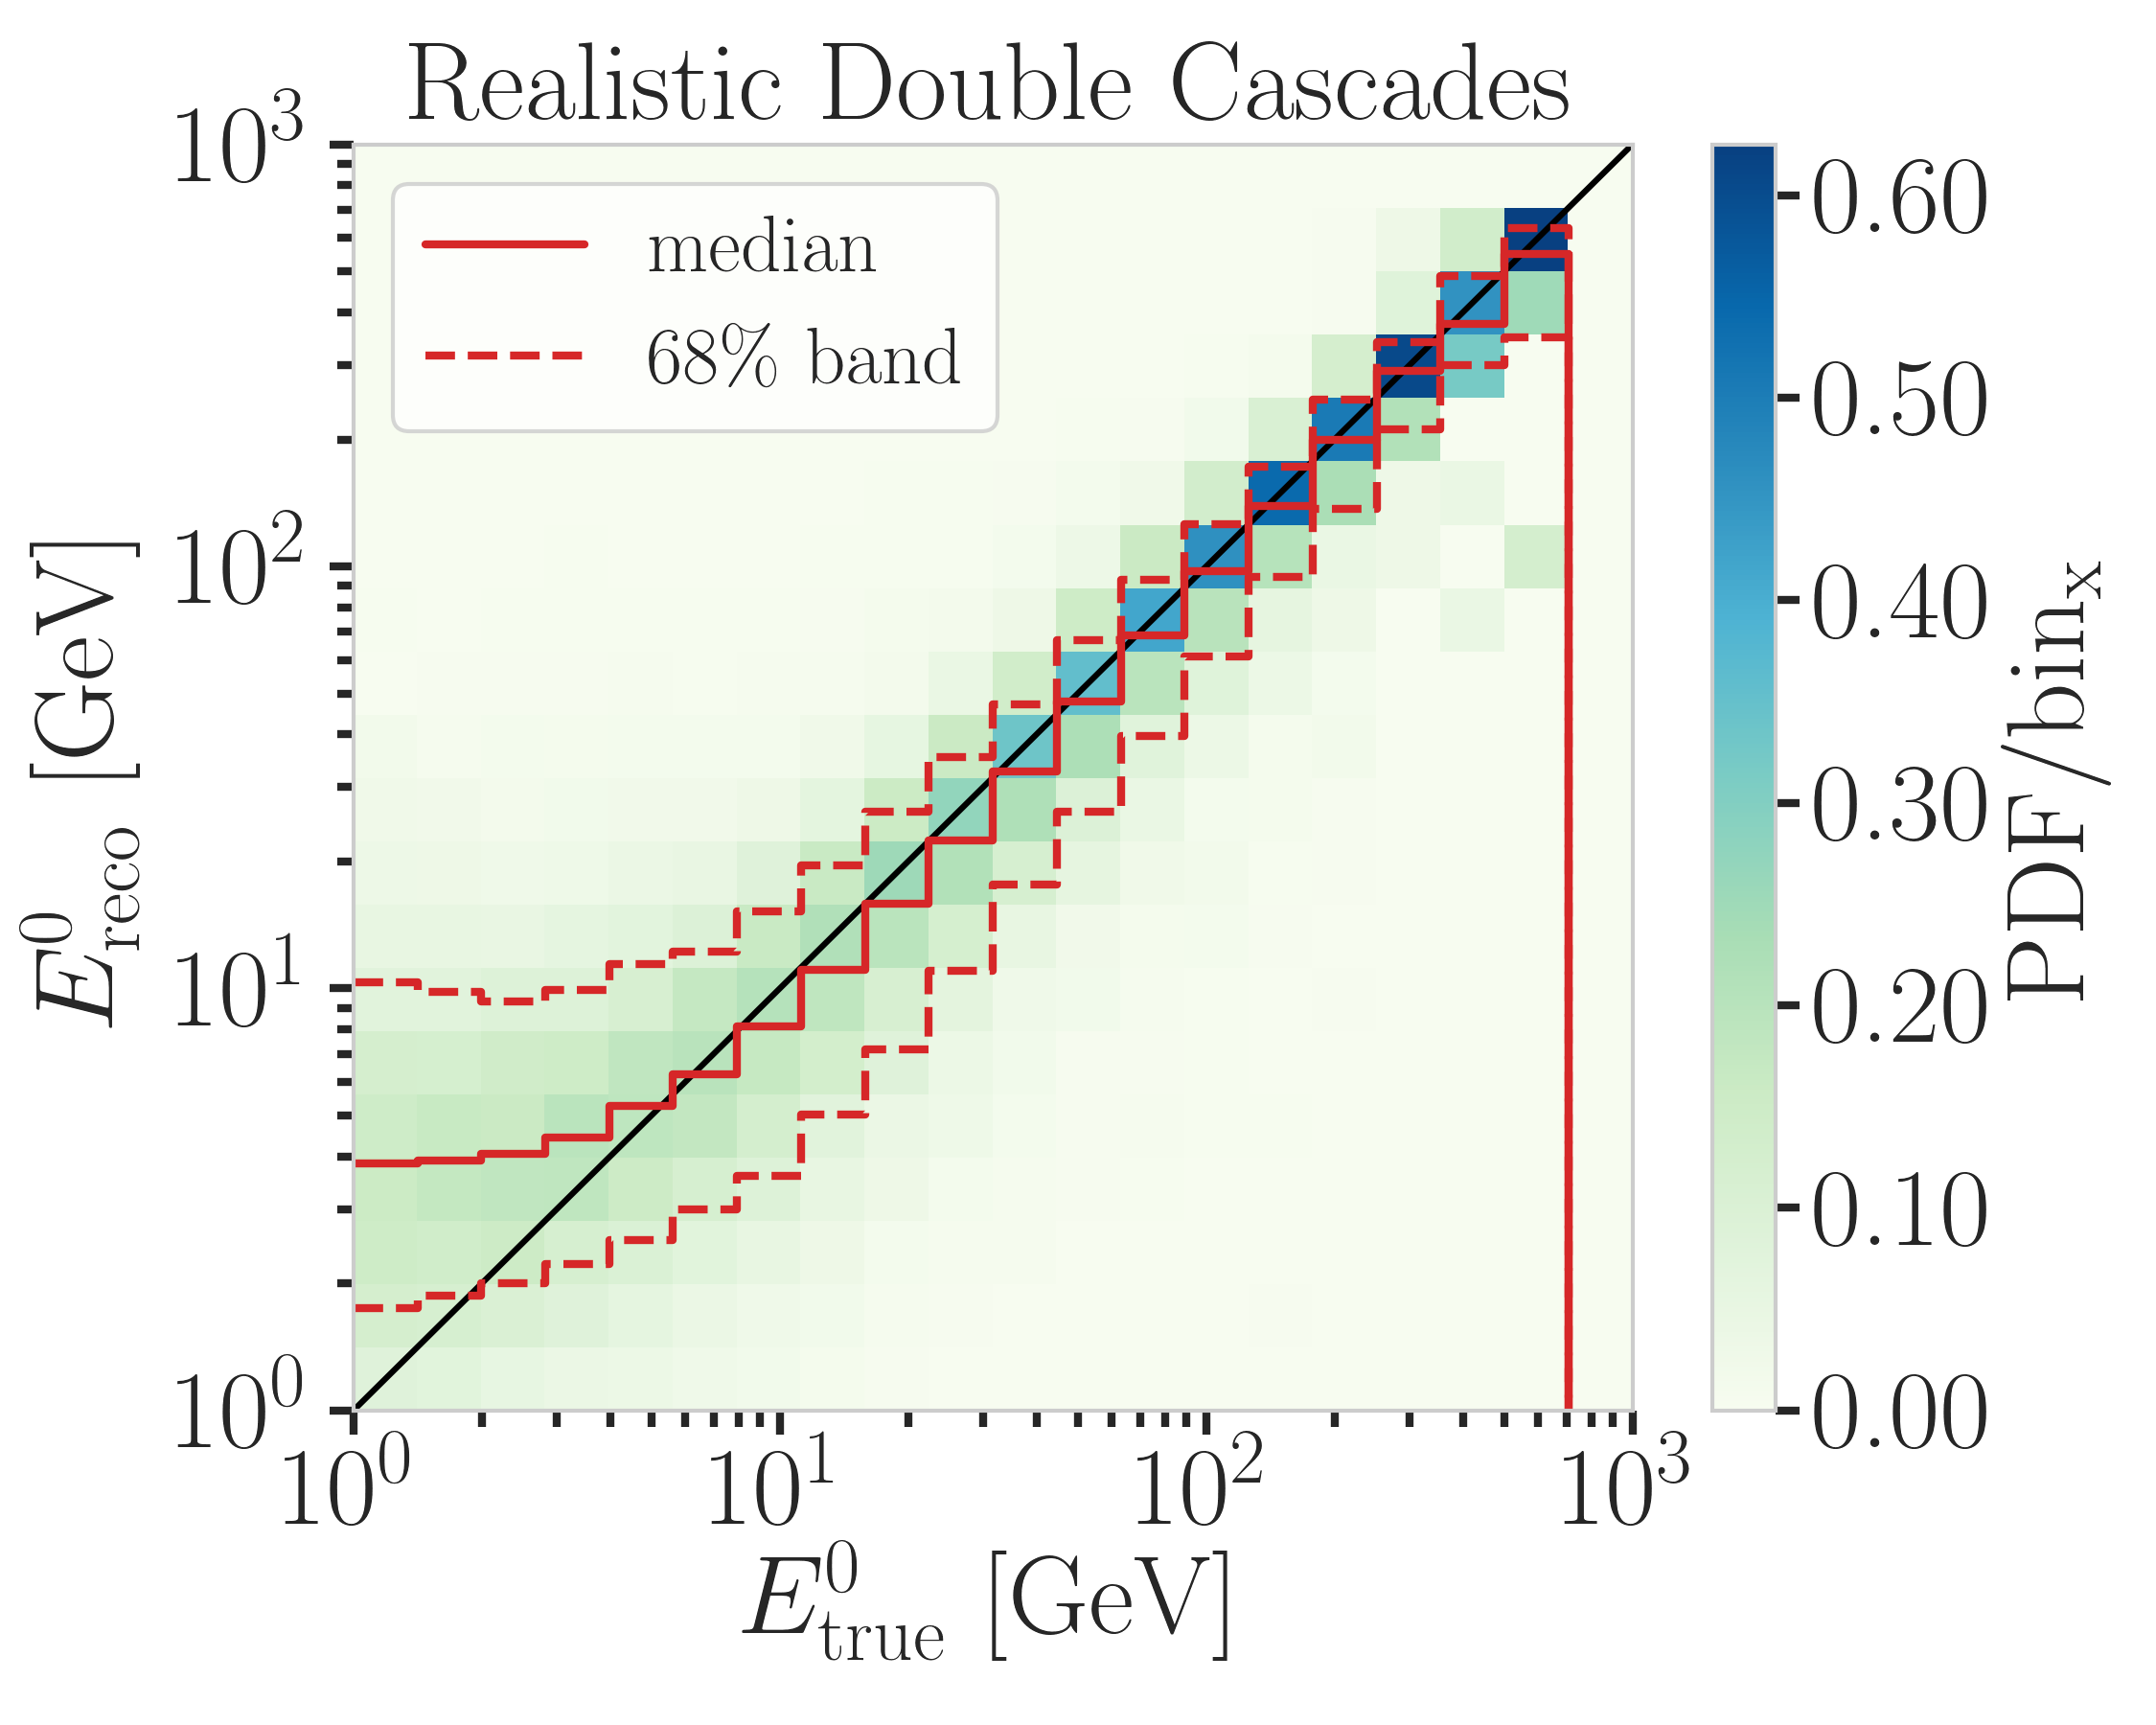
\includegraphics[width=0.49\linewidth]{figures/model_independent_simulation/results/realistic/2d_hists/194603_casc0_reco_energy_vs_casc0_true_energy_goodfit_step_contours.png}
    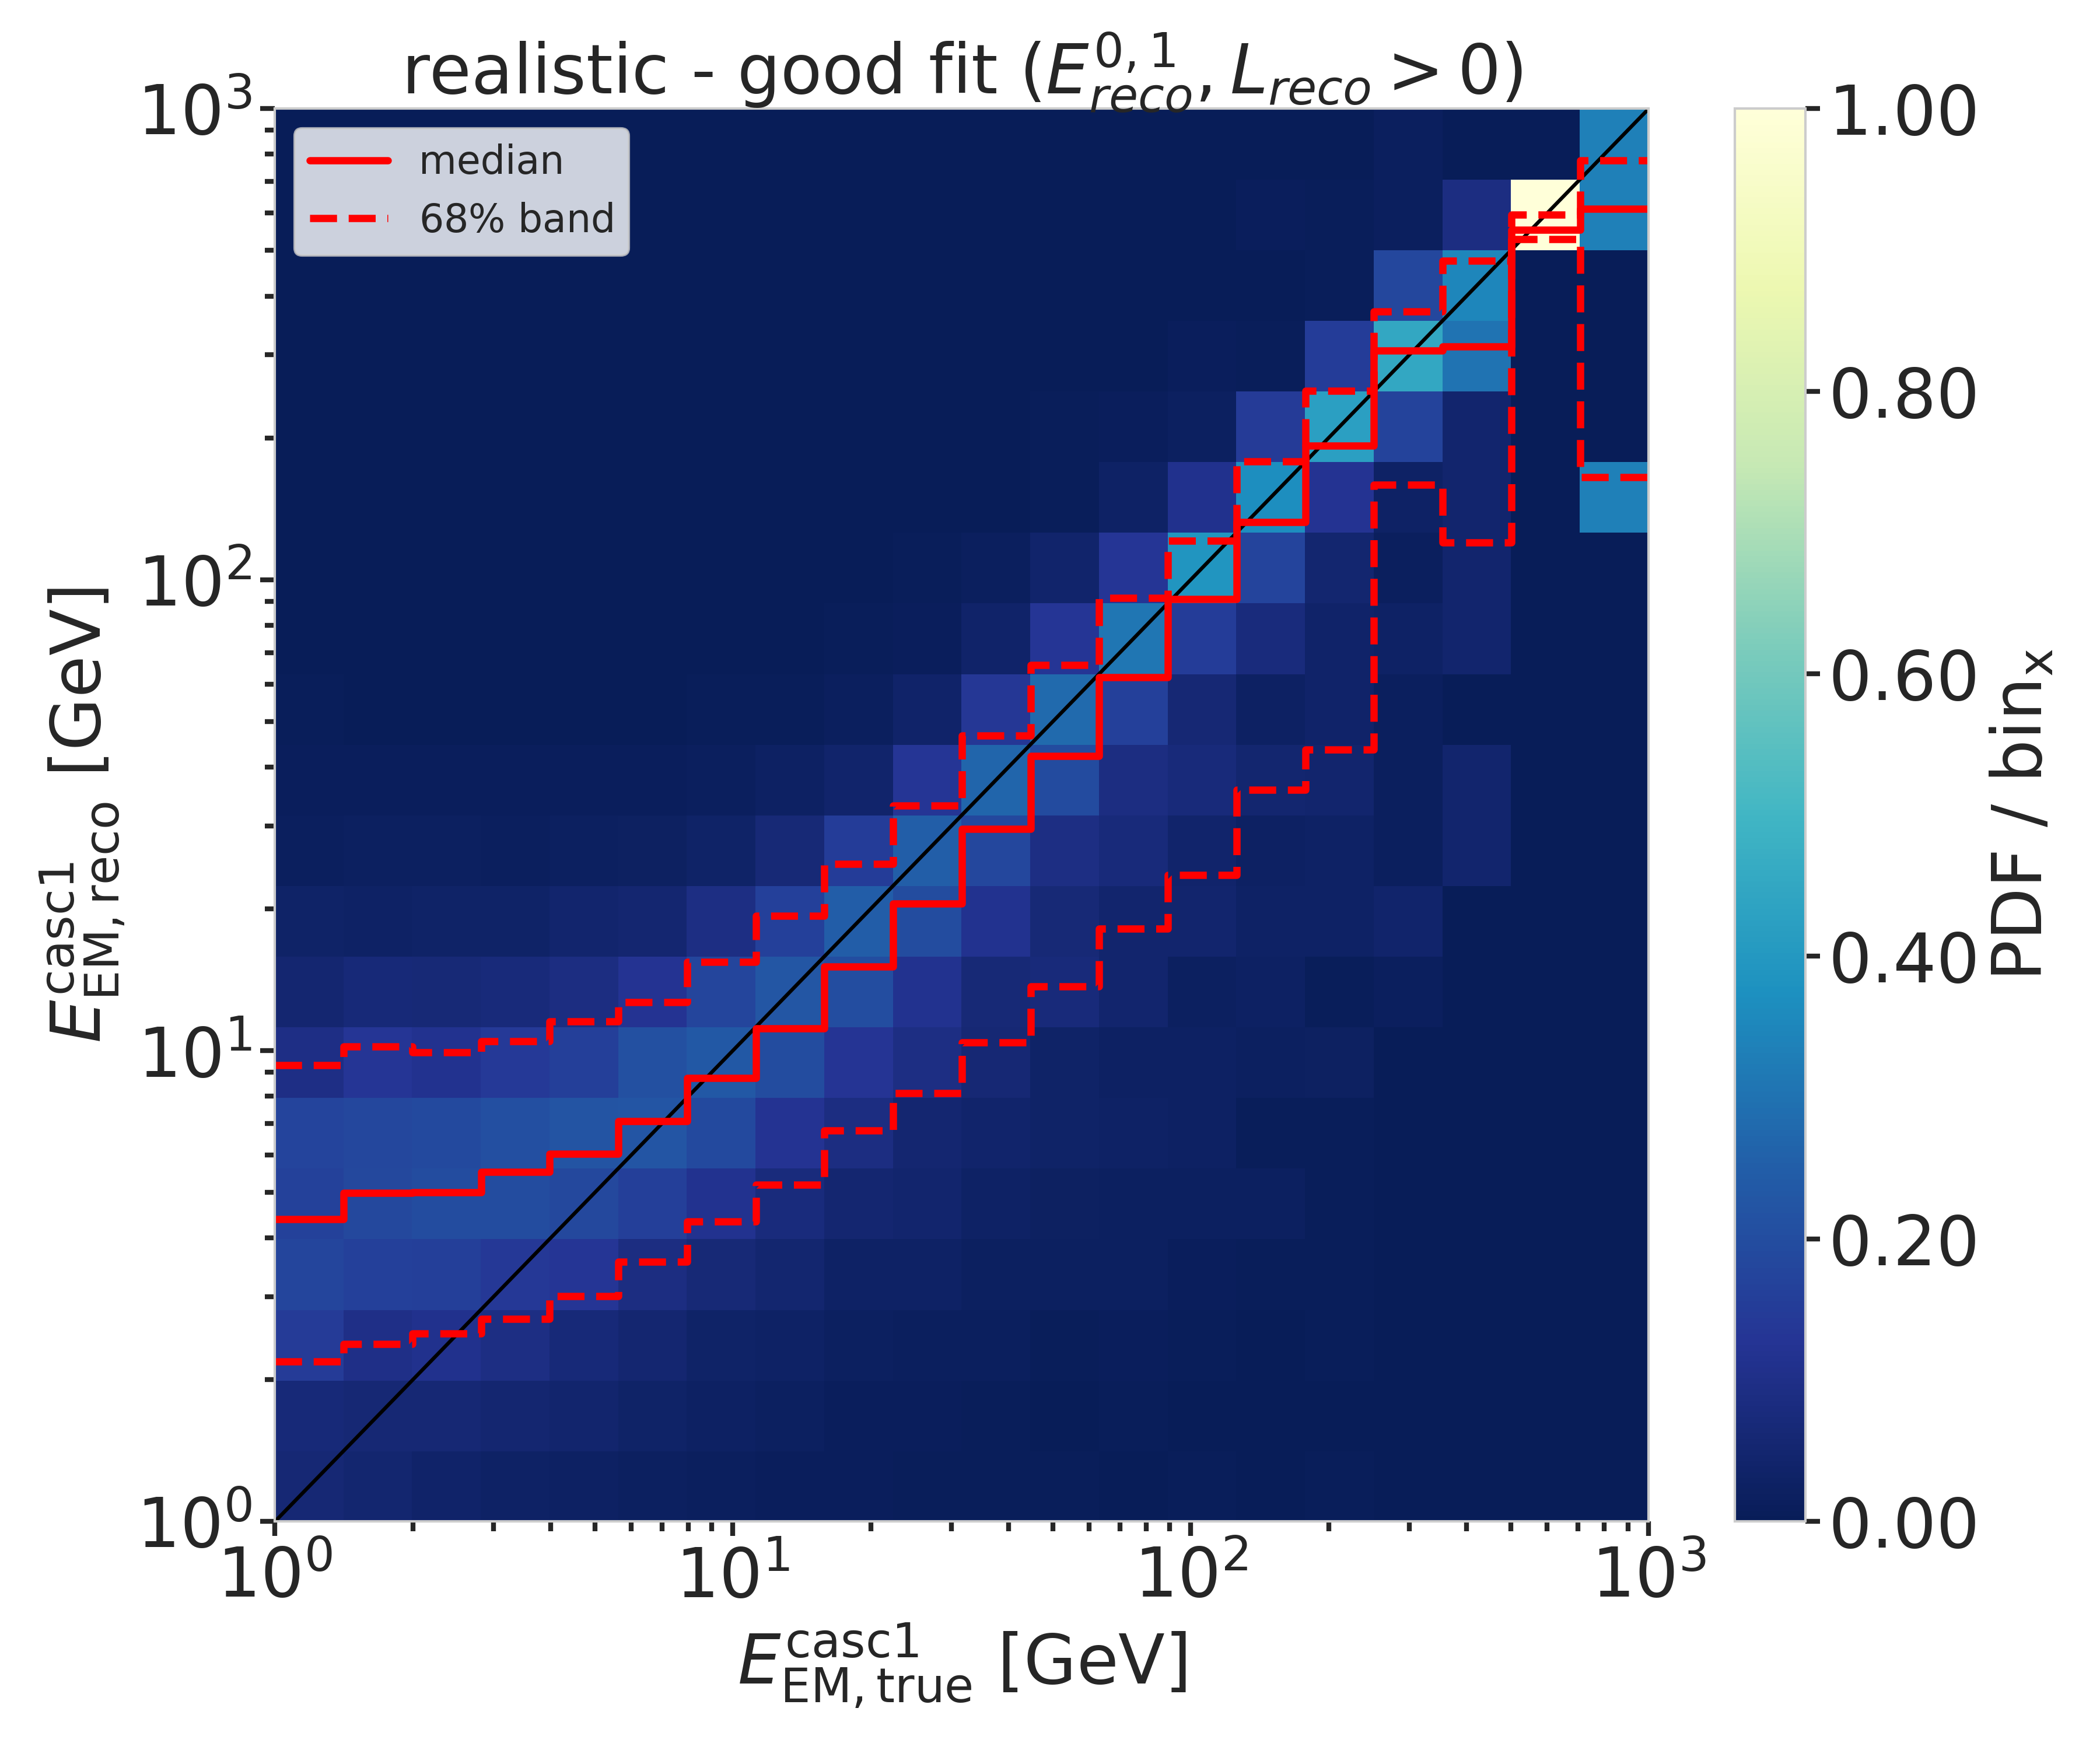
\includegraphics[width=0.49\linewidth]{figures/model_independent_simulation/results/realistic/2d_hists/194603_casc1_reco_energy_vs_casc1_true_energy_goodfit_step_contours.png}
    \caption[Realistic double-cascade energy resolutions]{Energy resolutions of the realistic, model-independent simulation sample. Shown is the reconstructed energy versus the true energy for both cascades, where the color scale is normalized per vertical slice and the median and \SI{68}{\percent} band are shown in red.}
    \labfig{cascade_energy_2dhists}
\end{figure*}


\paragraph{Decay Length Resolutions:}

The reconstructed decay length versus the true decay length is shown for all events in the left part of \reffig{realistic_sample_decay_length_2dhists}. For short true decay lengths the reconstruction is over-estimating the length, while for long true decay lengths the reconstruction is strongly under-estimating the length. There is a region between true decay lengths of \SIrange[range-phrase=~and~]{15}{80}{\meter} where the median reconstruction is almost unbiased, but the \SI{68}{\percent} interquartile range is wide with a lot of outliers towards short reconstructed lengths. Below \SI{15}{\meter} the reconstructed lengths are always over-estimating the true length and above \SI{80}{\meter} a population of events with short reconstructed length starts to dominate.

The over-estimation at small true decay lengths can be explained by multiple factors, one being that the shortest DOM spacing is $\sim$\SI{7}{\meter}, vertically for DeepCore strings, but mostly larger than that, so resolving lengths below that is very challenging. The reconstruction tends to be biased towards estimating the length around where the light was observed. Additionally, approaching a length of 0.0, the reconstructed length will of course always be a one-sided distribution, because the lengths have to be positive.

\begin{figure*}[h]
	\centering
    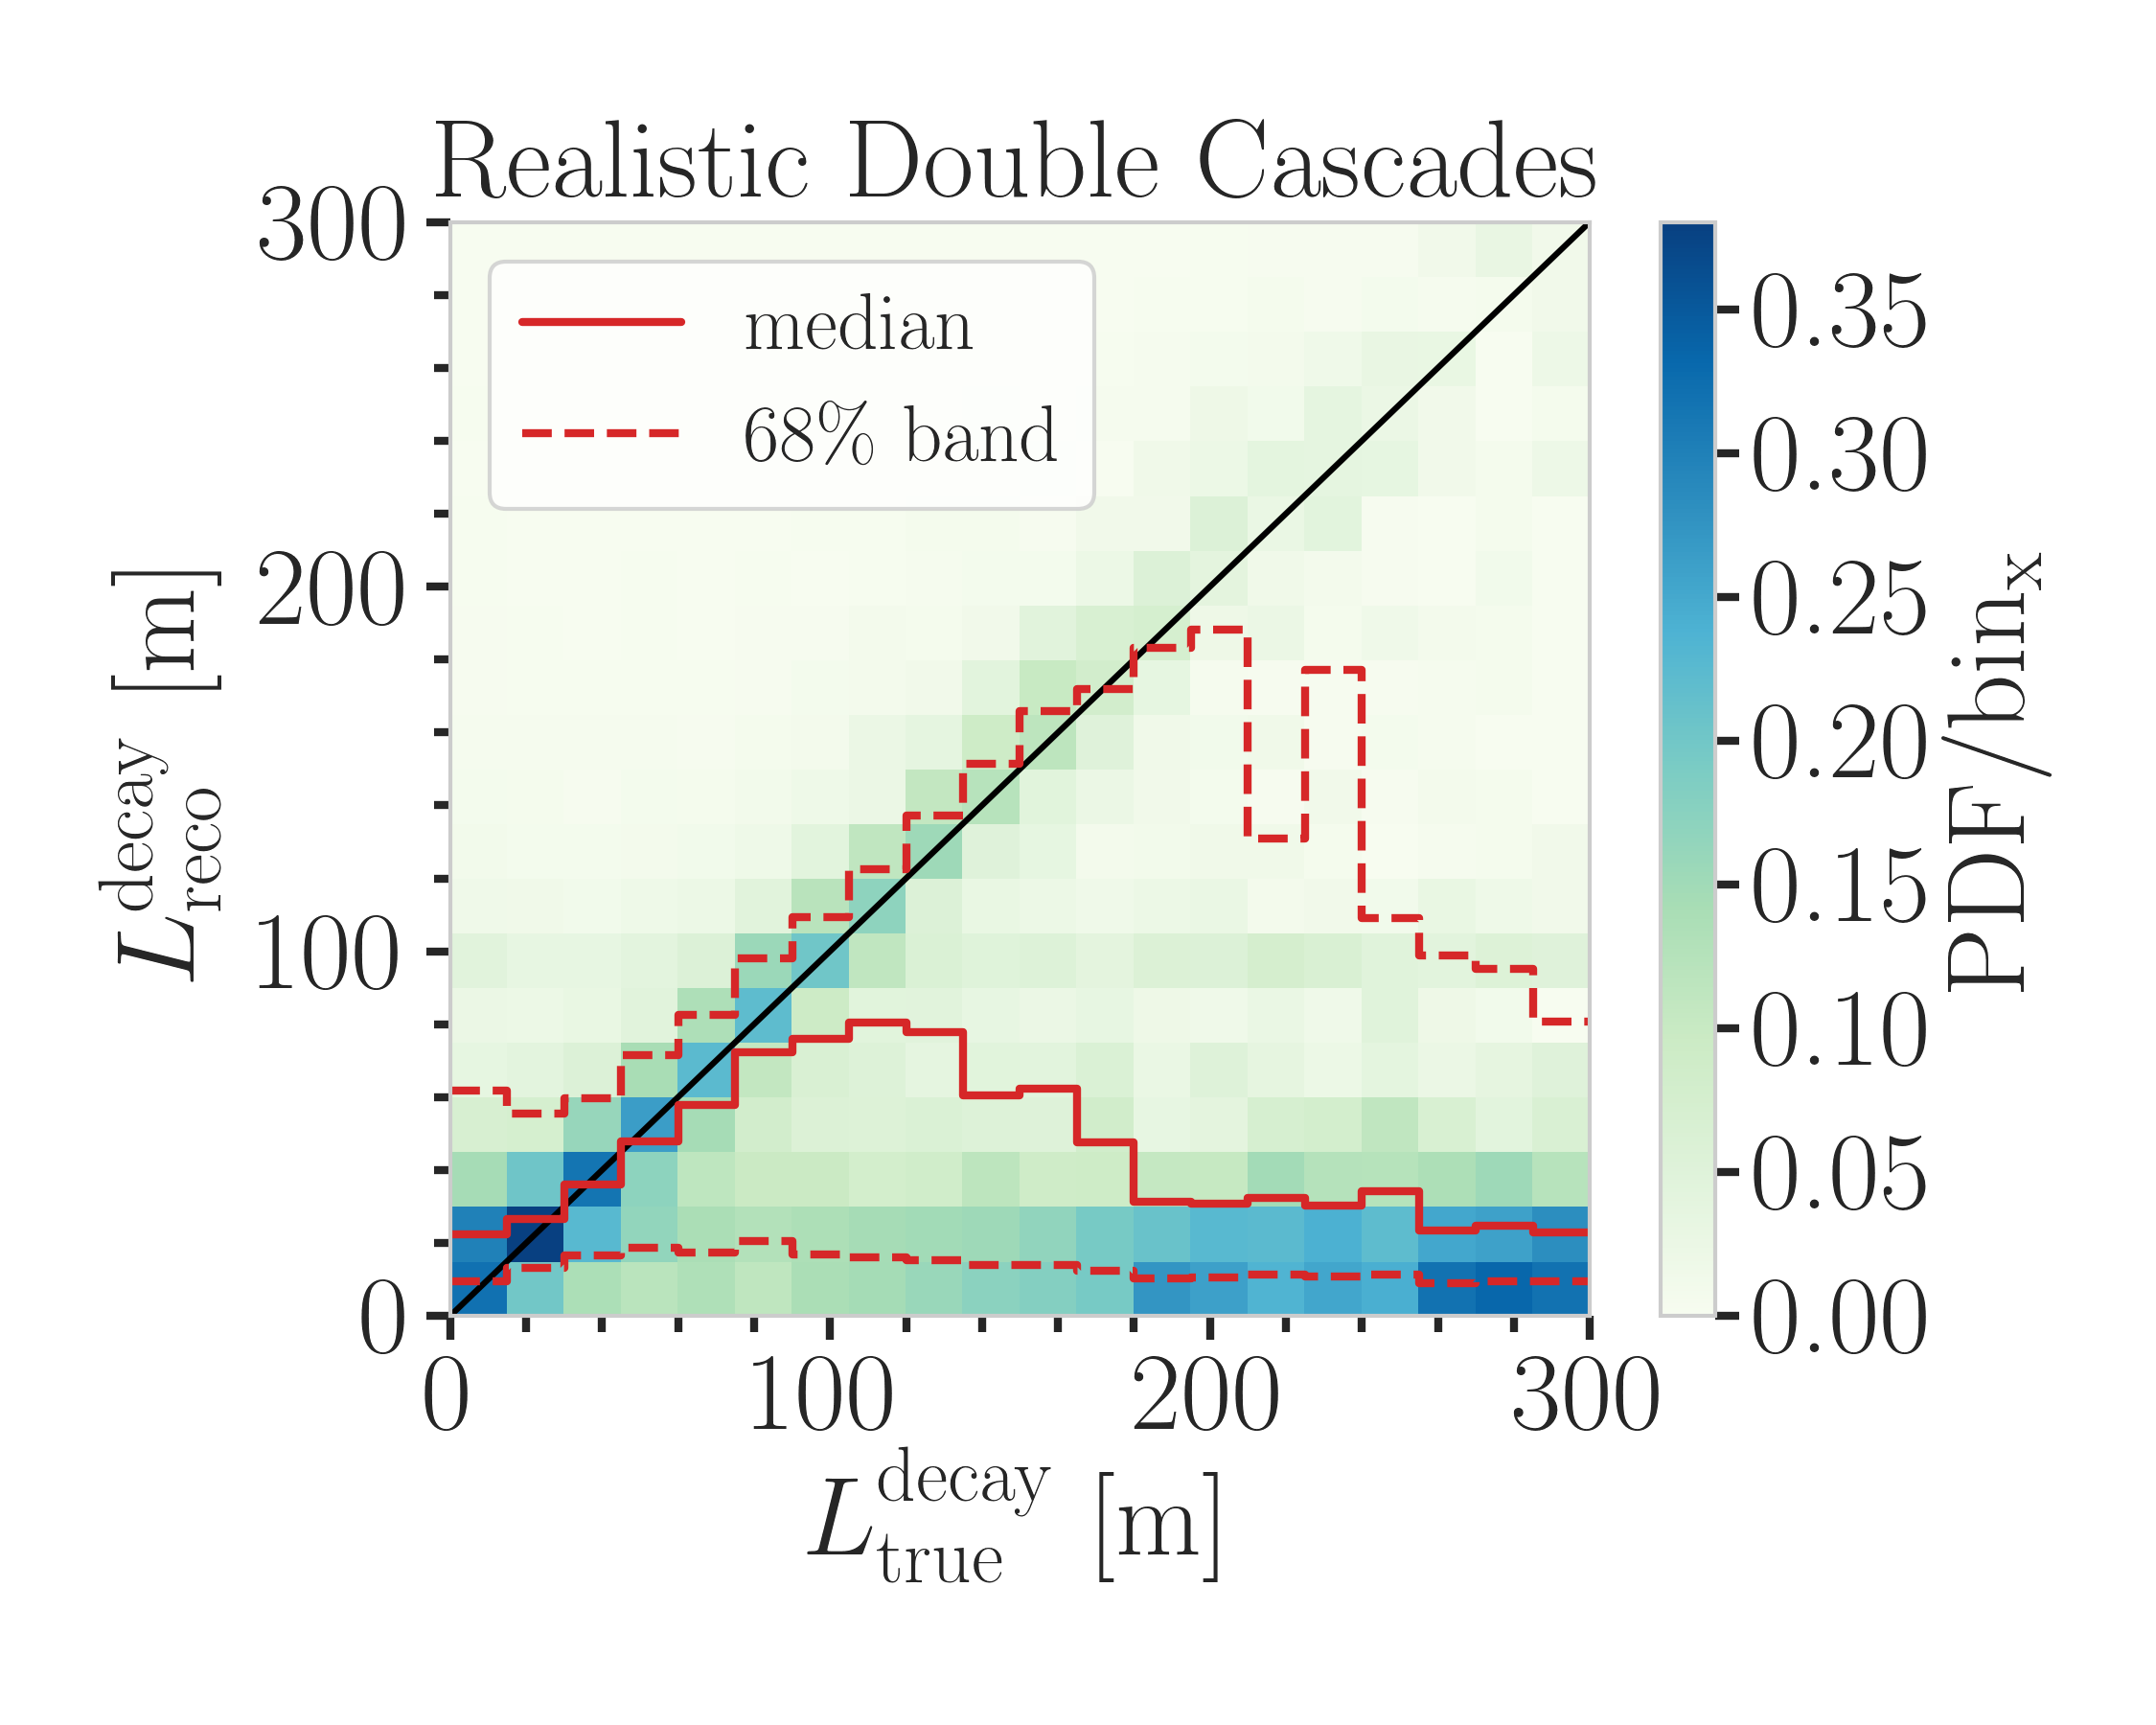
\includegraphics[width=0.49\linewidth]{figures/model_independent_simulation/results/realistic/2d_hists/194603_reco_decay_length_vs_true_decay_length_goodfit_step_contours.png}
    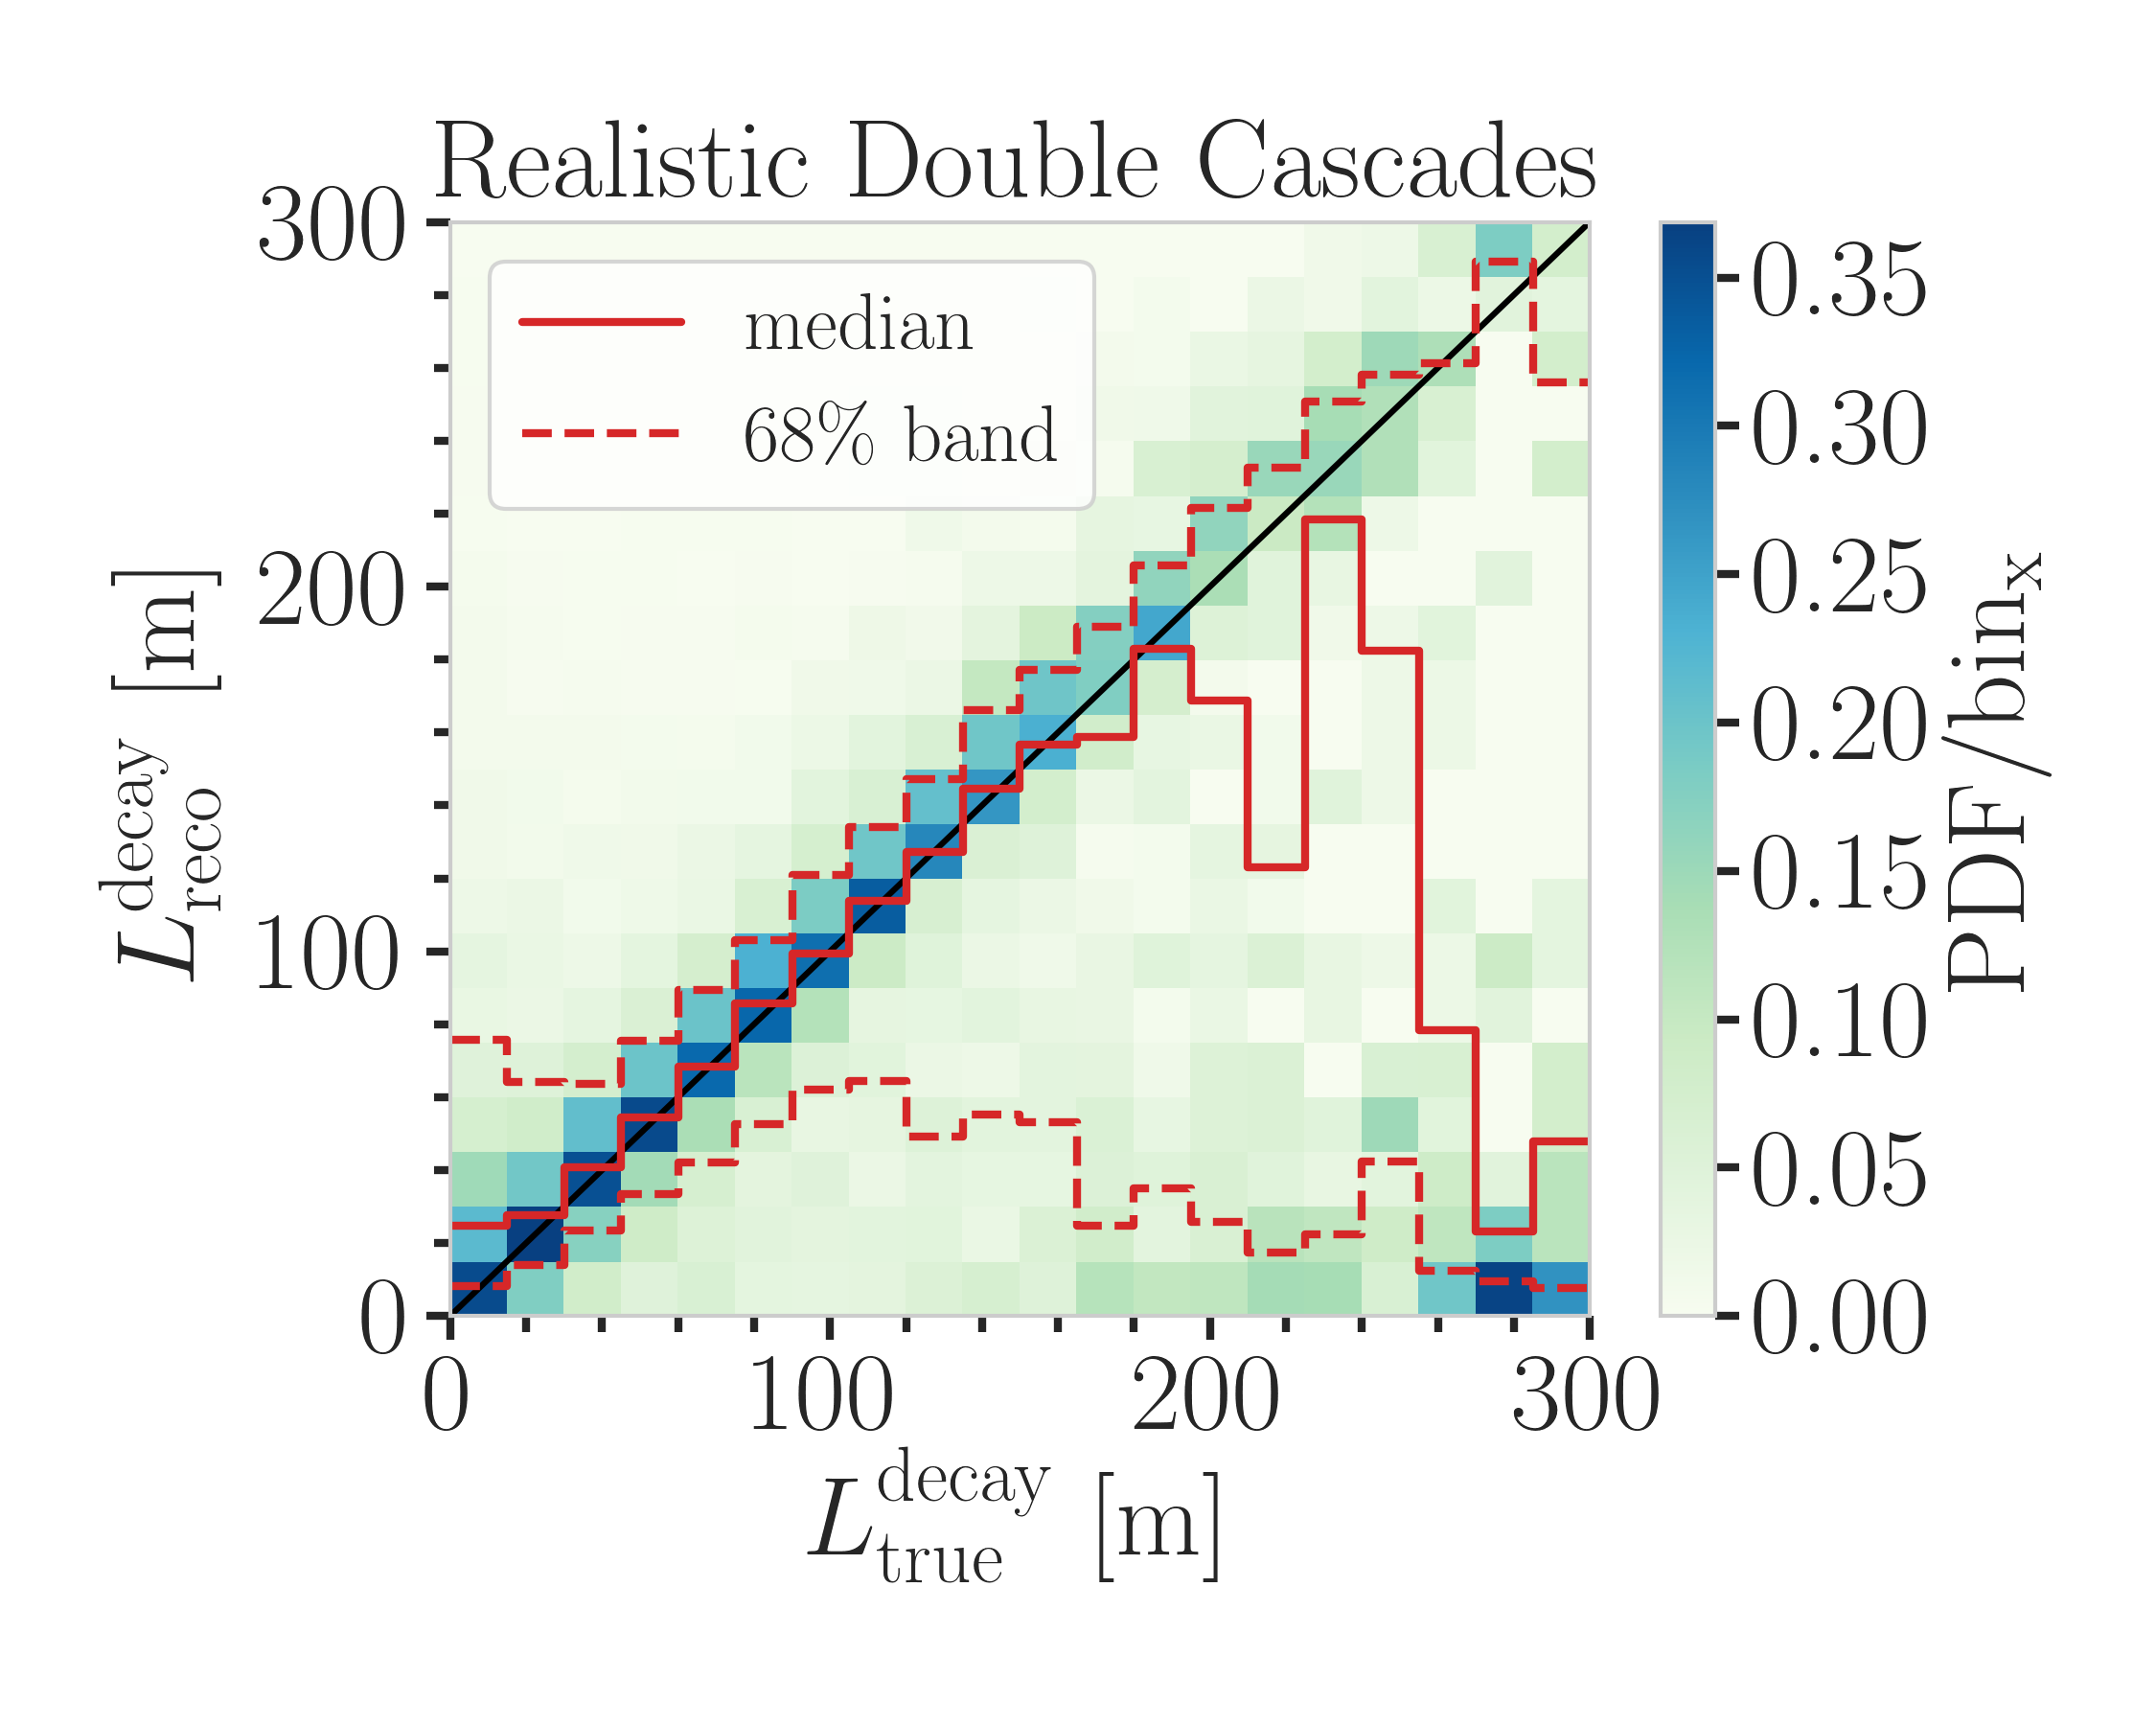
\includegraphics[width=0.49\linewidth]{figures/model_independent_simulation/results/realistic/2d_hists/194603_reco_decay_length_vs_true_decay_length_goodfit_above_10_GeV_step_contours}
    \caption[Realistic double-cascade length resolution]{Length resolution of the realistic, model-independent simulation sample. Shown is the two-dimensional histograms of the reconstructed length versus the true length for all events (left) and for events with reconstructed cascade energies larger than \SI{10}{\gev} (right), where the color scale is normalized per vertical slice and the median and \SI{68}{\percent} band are shown in red.}
    \labfig{realistic_sample_decay_length_2dhists}
\end{figure*}

The under-estimation at large true decay lengths is more puzzling. It seems like the distribution becomes bimodal in the reconstructed lengths. There is one well reconstructed population around the diagonal, and another badly reconstructed population at very short reconstructed lengths. Above \SI{150}{\meter} the badly reconstructed population starts to dominate, and the median resolution drops off strongly. For these events, only one cascade was observed with enough light to be reconstructed, and the reconstruction describes the one observed cascade in two parts, separated by a short distance. The result of applying a minimum energy cut on the reconstructed cascade energies ($E^0, E^1 \ge \SI{10}{\gev}$) is shown in the right part of \reffig{realistic_sample_decay_length_2dhists}. It can be seen that the median resolution improves significantly, now aligning with the expectation between \SIrange[range-phrase=~and~]{15}{160}{\meter}. The spread also improves, but is still biased towards short reconstructed lengths and above \SI{200}{\meter} the badly reconstructed population starts to dominate again.


\paragraph{Resolution Benchmarks:}

\begin{figure*}[h]
	\centering
    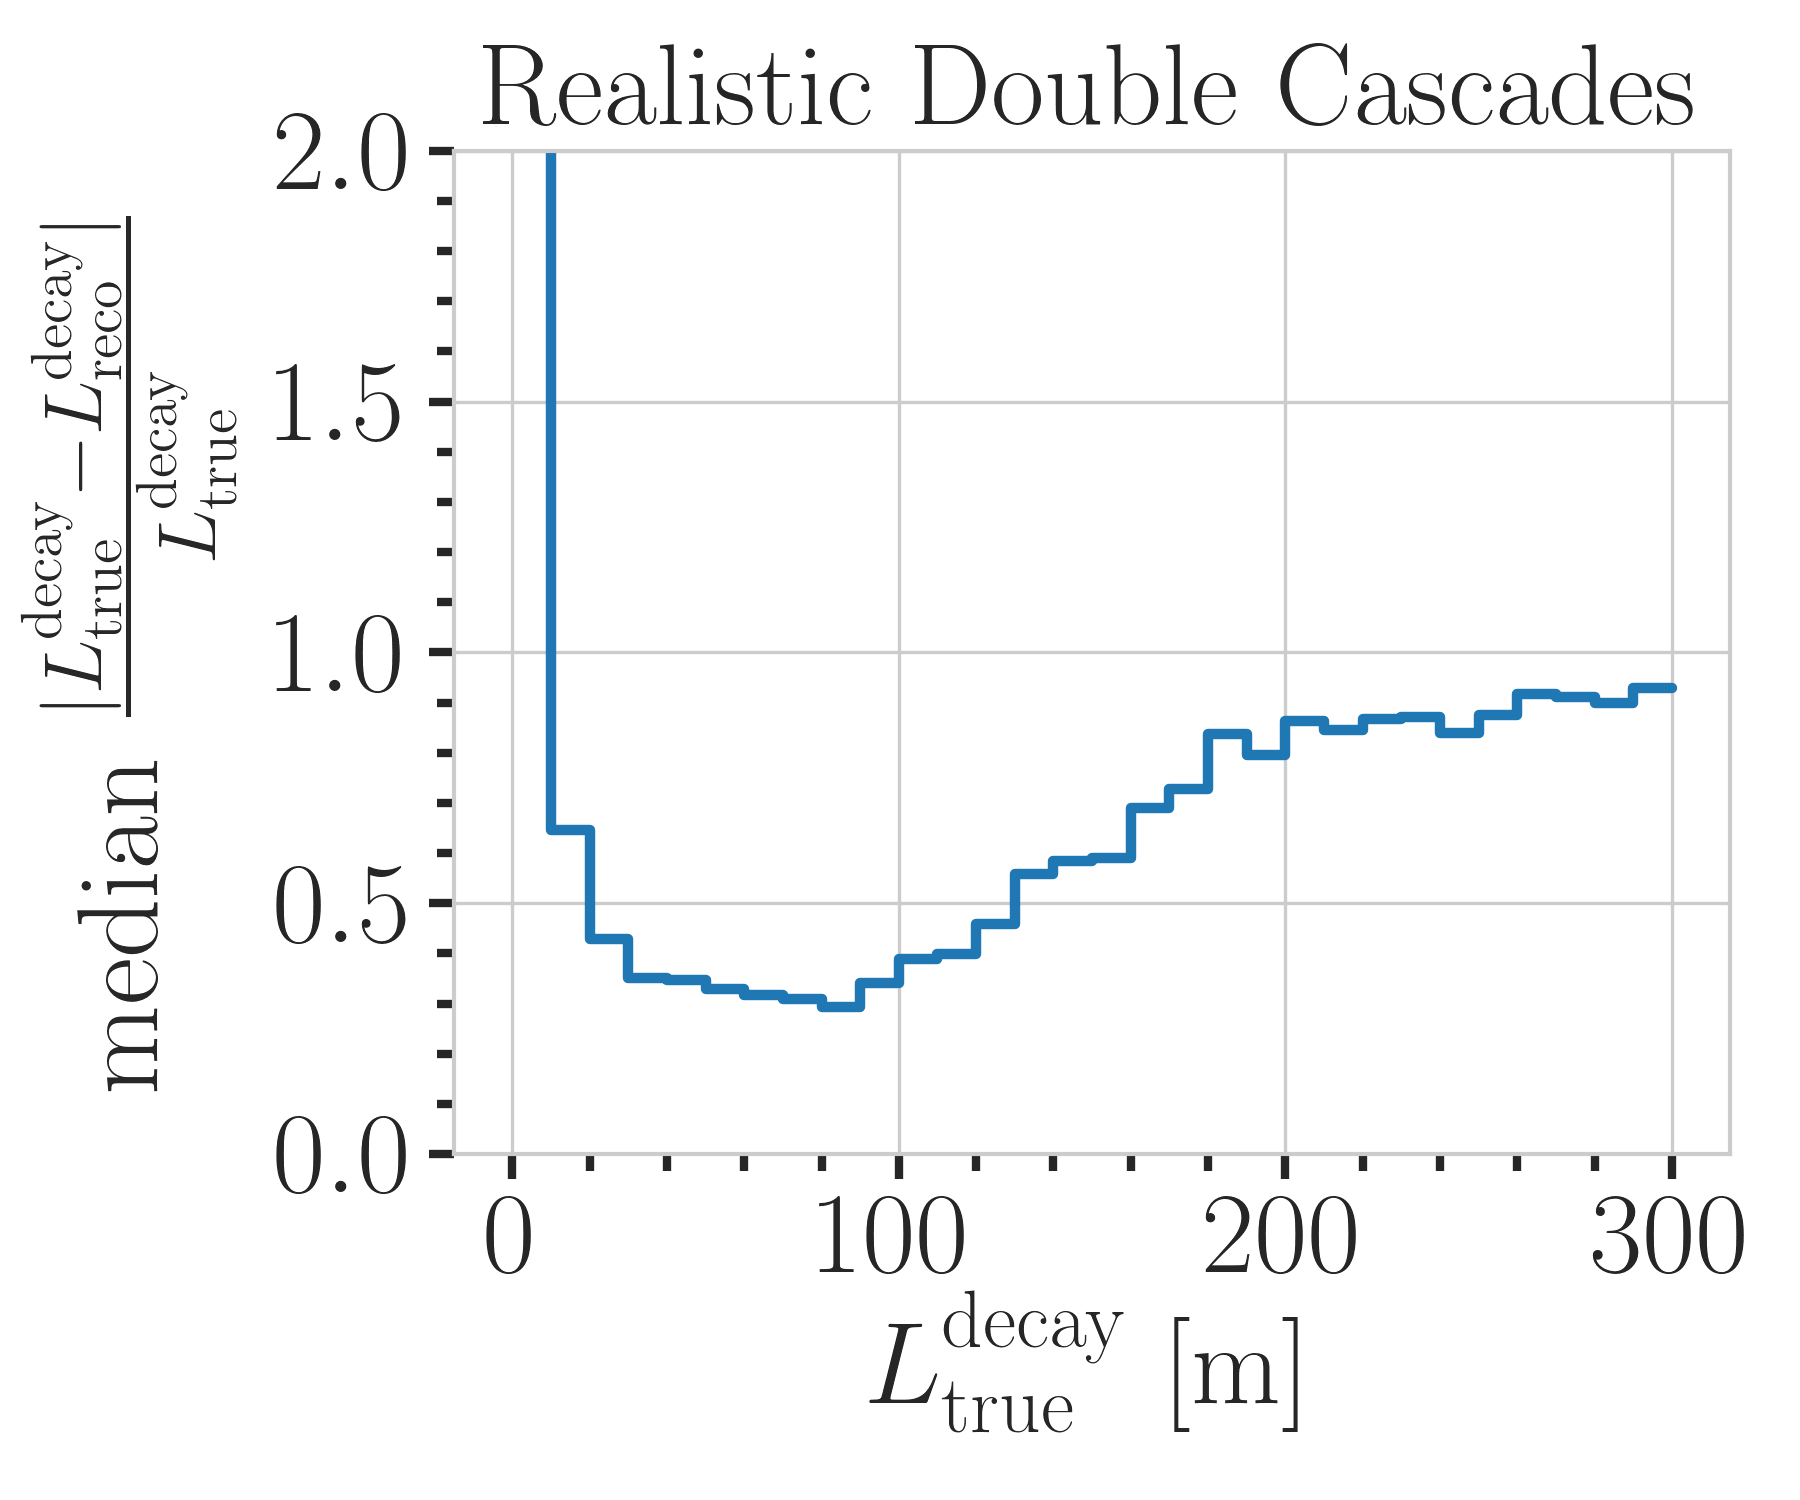
\includegraphics[width=0.45\linewidth]{figures/model_independent_simulation/results/realistic/resolutions/194603_median_decay_length_resolution_goodfit_log_unweighted.png}
    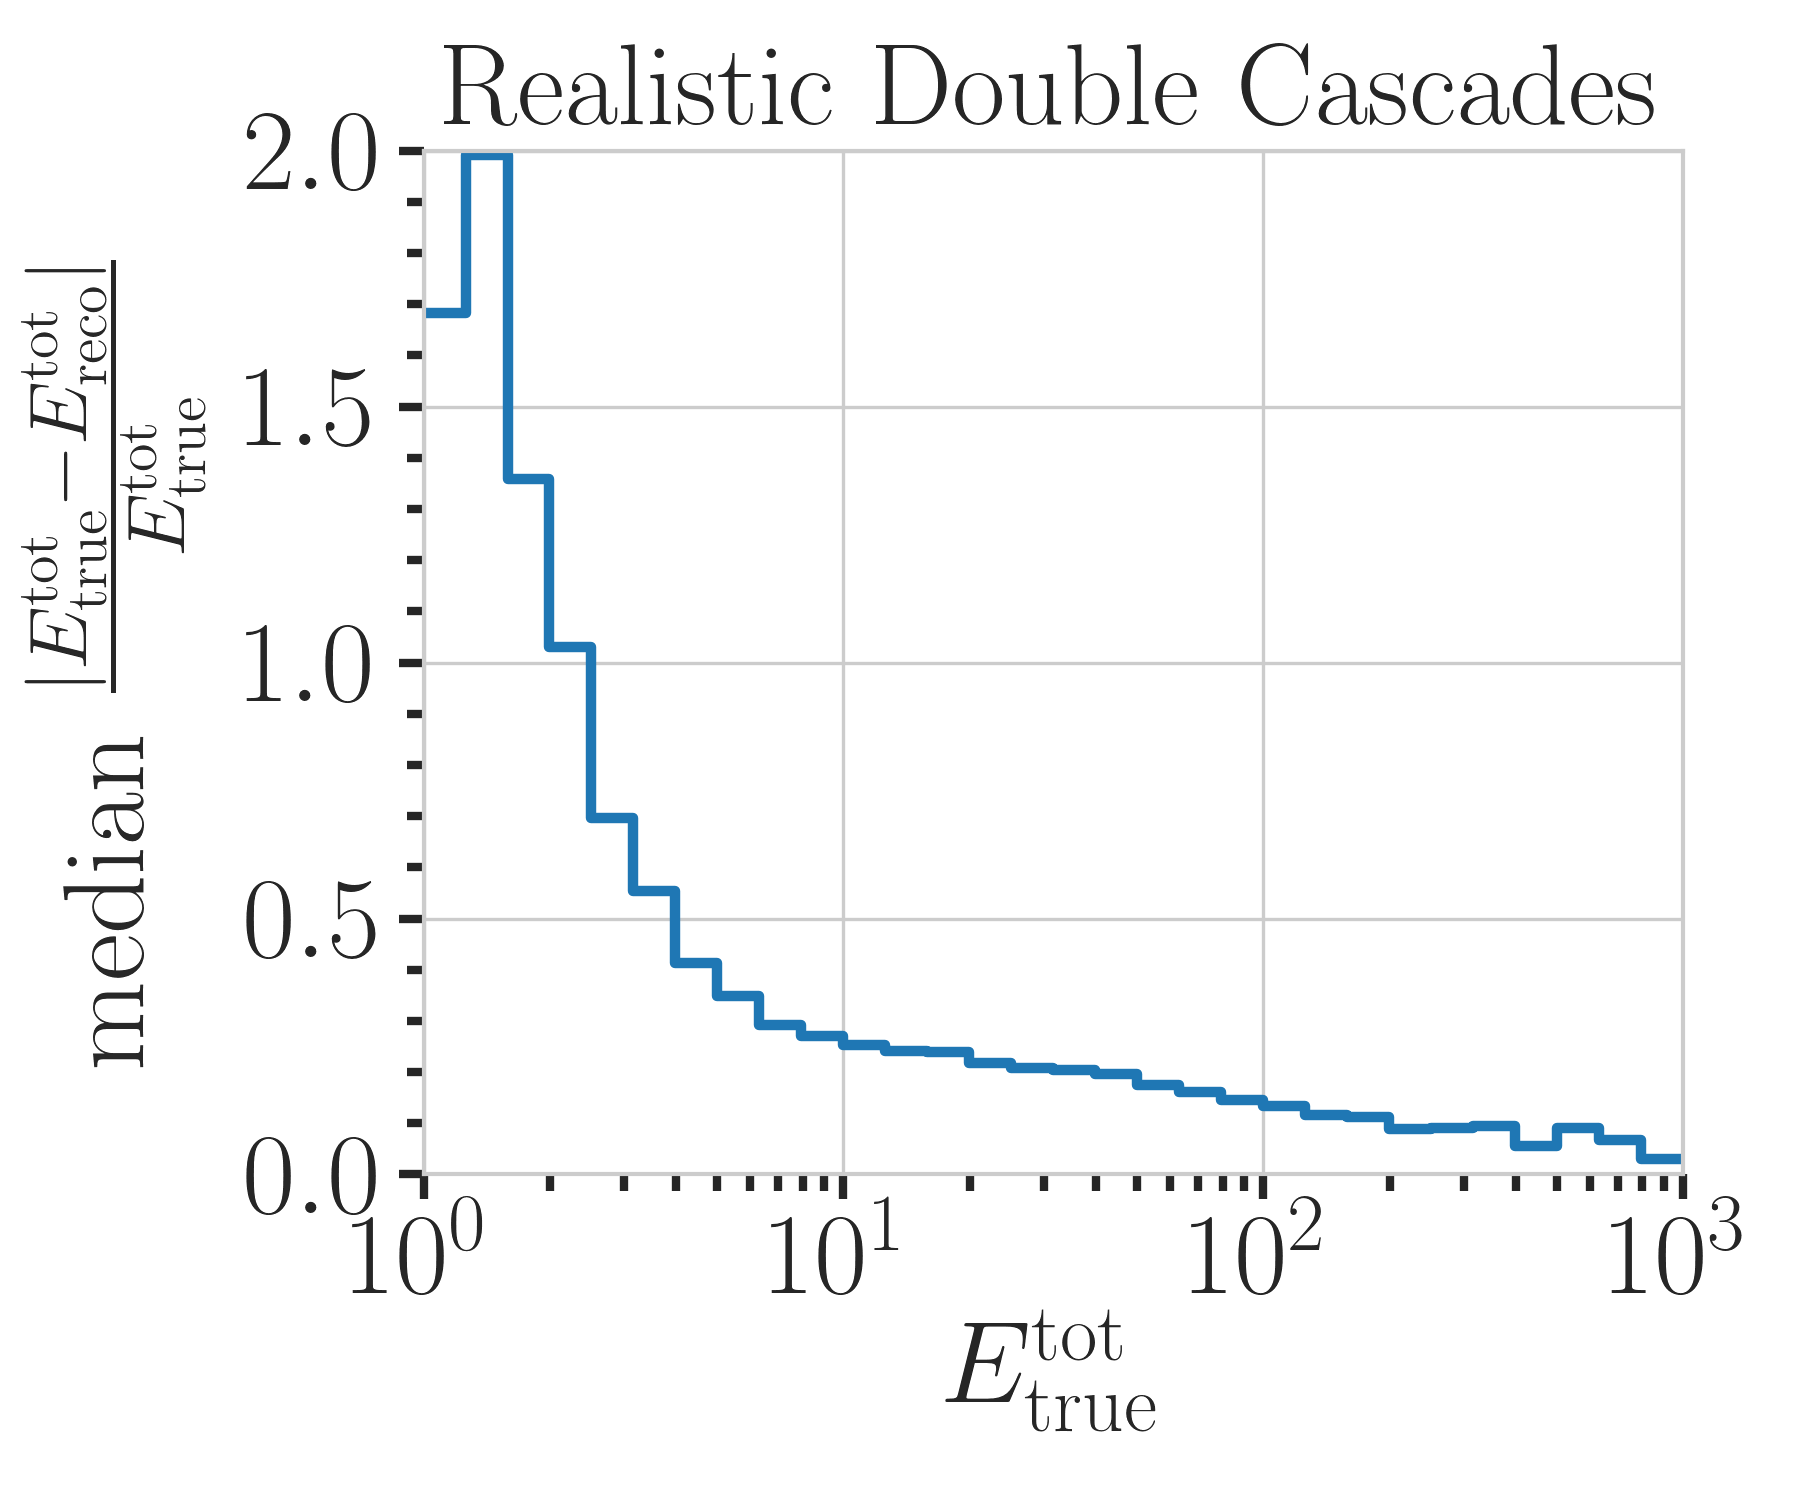
\includegraphics[width=0.45\linewidth]{figures/model_independent_simulation/results/realistic/resolutions/194603_median_absolute_fractional_reco_total_energy_error_goodfit.png} 
    \caption[Realistic double-cascade decay length and total energy resolution]{Decay length and total energy resolution of events from the realistic sample. Shown is the decay length resolution as a function of the true decay length (left) and the total energy resolution as a function of the true total energy (right).}
    \labfig{median_resolutions_energy_length}
\end{figure*}

The left part of \reffig{median_resolutions_energy_length} shows the median resolutions of the decay length as a function of the true decay length. It falls below \SI{65}{\percent} above a true decay length of $\sim$\SI{10}{\meter}, and starts to increase again with increasing true length around \SI{100}{\meter}, where it is at \SI{40}{\percent}. For larger true decay length, where the badly reconstructed population dominates, the resolution is large, stabilizing at around \SI{90}{\percent} at \SI{200}{\meter}. This is a significantly worse behavior than the performance found for the best-case event types shown in the left part of \reffig{idealistic_length_resolutions}. The total energy resolution versus the true total energy is shown in the right part of \reffig{median_resolutions_energy_length}. Above \SI{4}{\gev} it is good and constantly improving with the true total energy. It falls below \SI{30}{\percent} at \SI{10}{\gev} and reaches \SI{15}{\percent} at \SI{100}{\gev}.

\begin{figure*}[h]
	\centering
    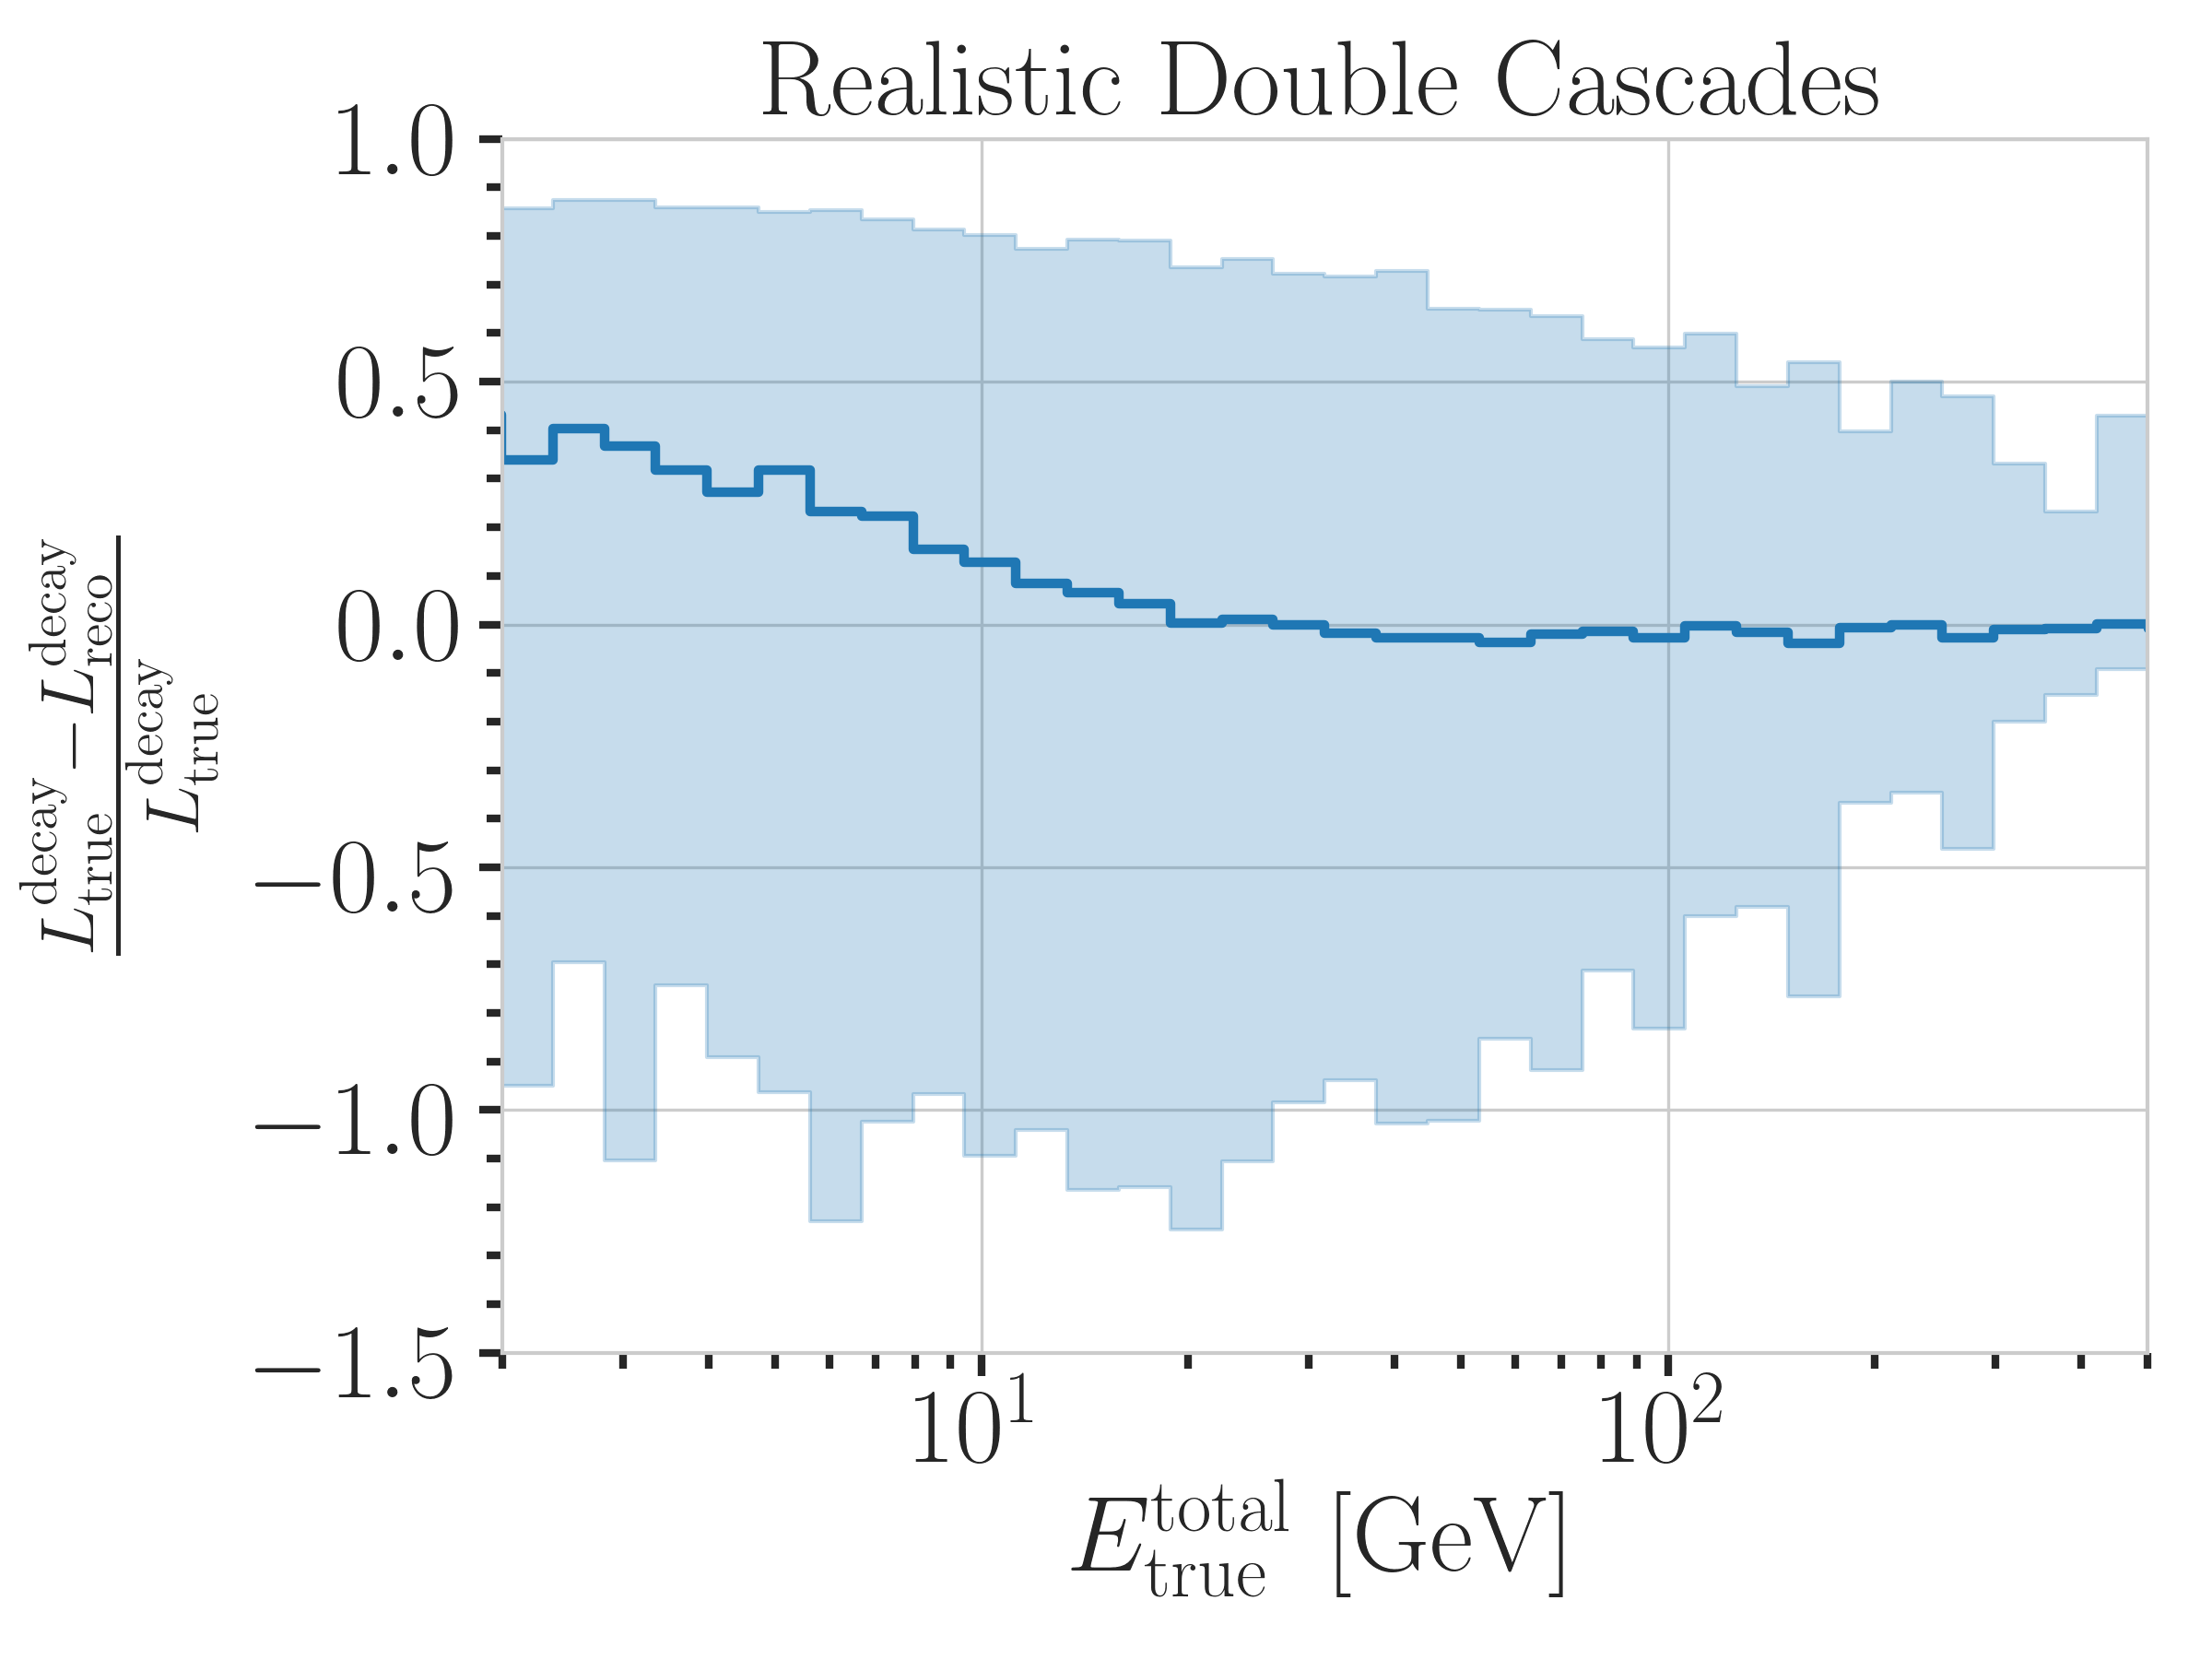
\includegraphics[width=0.49\linewidth]{figures/model_independent_simulation/results/realistic/resolutions/194603_median_decay_length_bias_vs_tot_energy_goodfit_log_unweighted.png}
    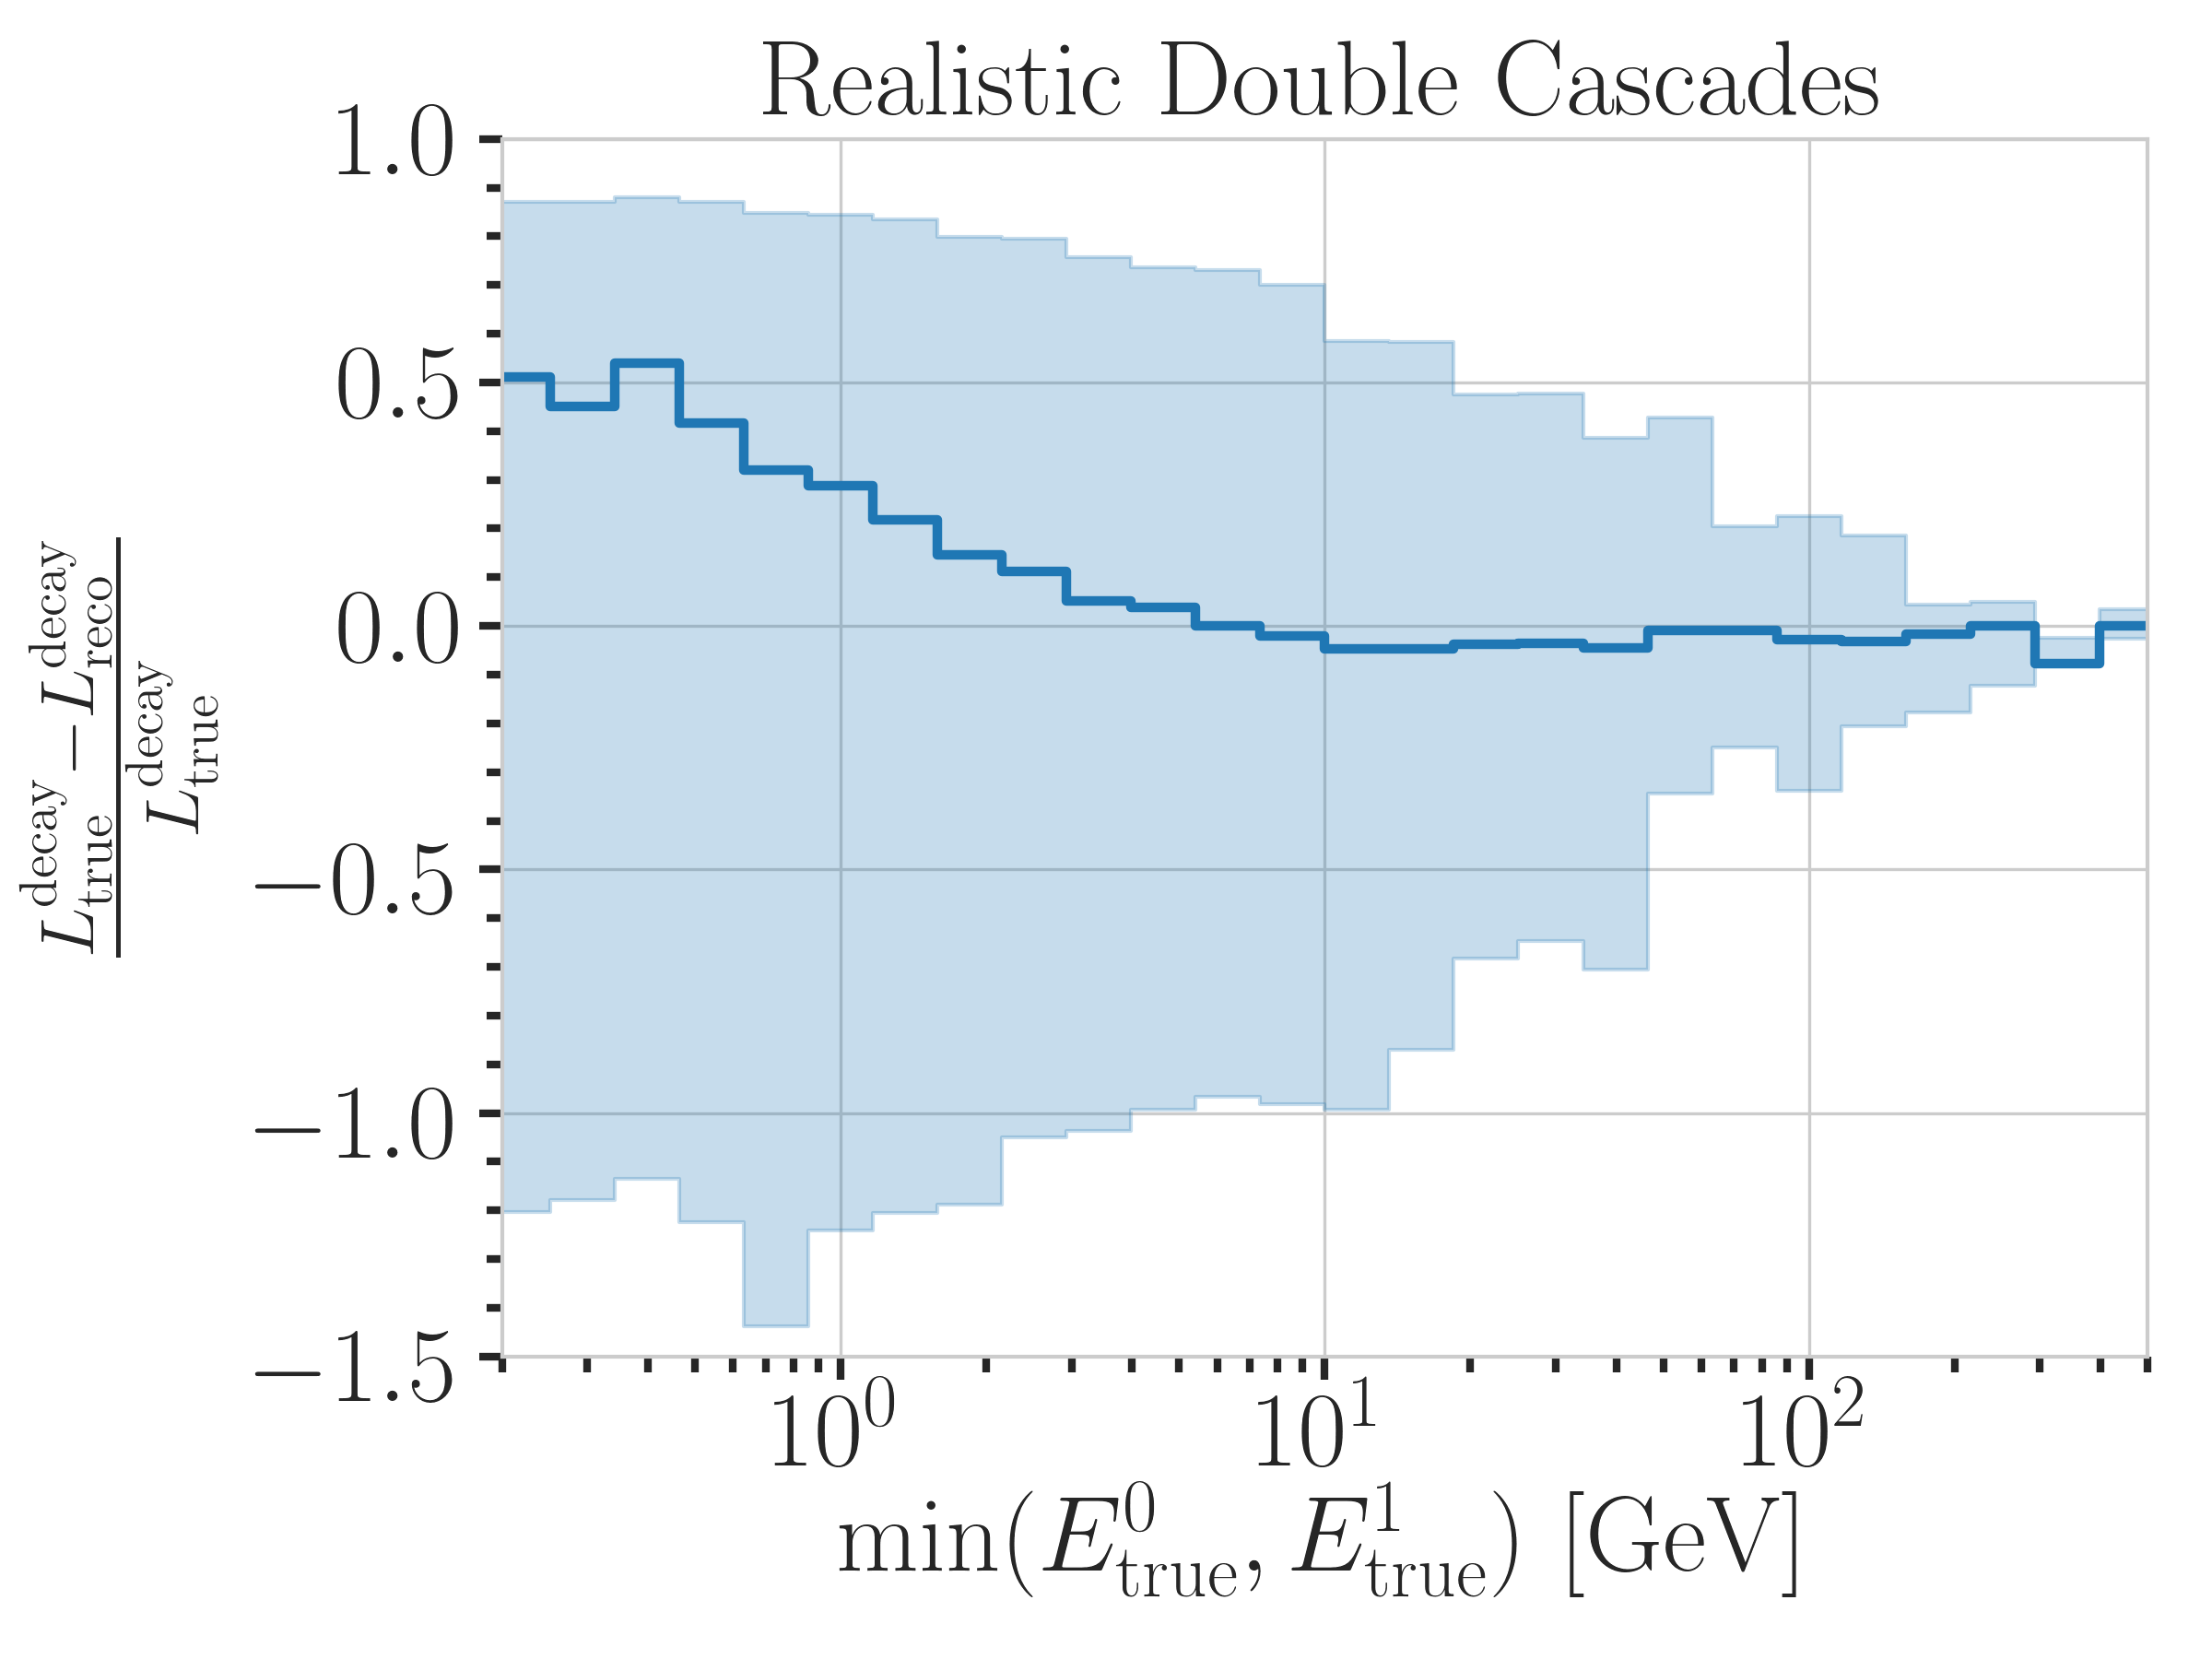
\includegraphics[width=0.49\linewidth]{figures/model_independent_simulation/results/realistic/resolutions/194603_median_decay_length_bias_vs_min_energy_goodfit_log_unweighted.png} 
    \caption[Realistic double-cascade decay length resolution versus energies]{Decay length resolution of events from the realistic sample. Shown is the decay length resolution as a function of the true total energy (left) and as a function of the minimum true energy of the cascades (right).}
    \labfig{decay_length_bias_vs_energies}
\end{figure*}

To get an estimate of what minimum energies are necessary for the reconstruction to perform reasonably well, the fractional decay length resolution is shown as a function of the total true energy and the minimum energy of both individual cascades in \reffig{decay_length_bias_vs_energies}. In the left part it can be seen that the median of the decay length resolution stabilizes around 0 for a total energy above \SI{20}{\gev}, but the spread of the distribution is still quite large with a \SI{68}{\percent} band of \SIrange{80}{100}{\percent}, decreasing down to $\sim$\SI{60}{\percent} at \SI{100}{\gev}. The right part of the figure shows the decay length resolution as a function of the minimum true energy of the cascades. The decay length resolution starts to be unbiased for a minimum energy of any cascade of \SI{7}{\gev}, with an equivalently large spread. A rough takeaway from this is that the decay length reconstruction is not reliable for events with one cascade energy below \SI{7}{\gev} and with a total energy below \SI{20}{\gev}. Above these values the median resolution is roughly unbiased, but the spread is still large, decreasing with increasing energy.


\begin{figure*}[h]
	\centering
    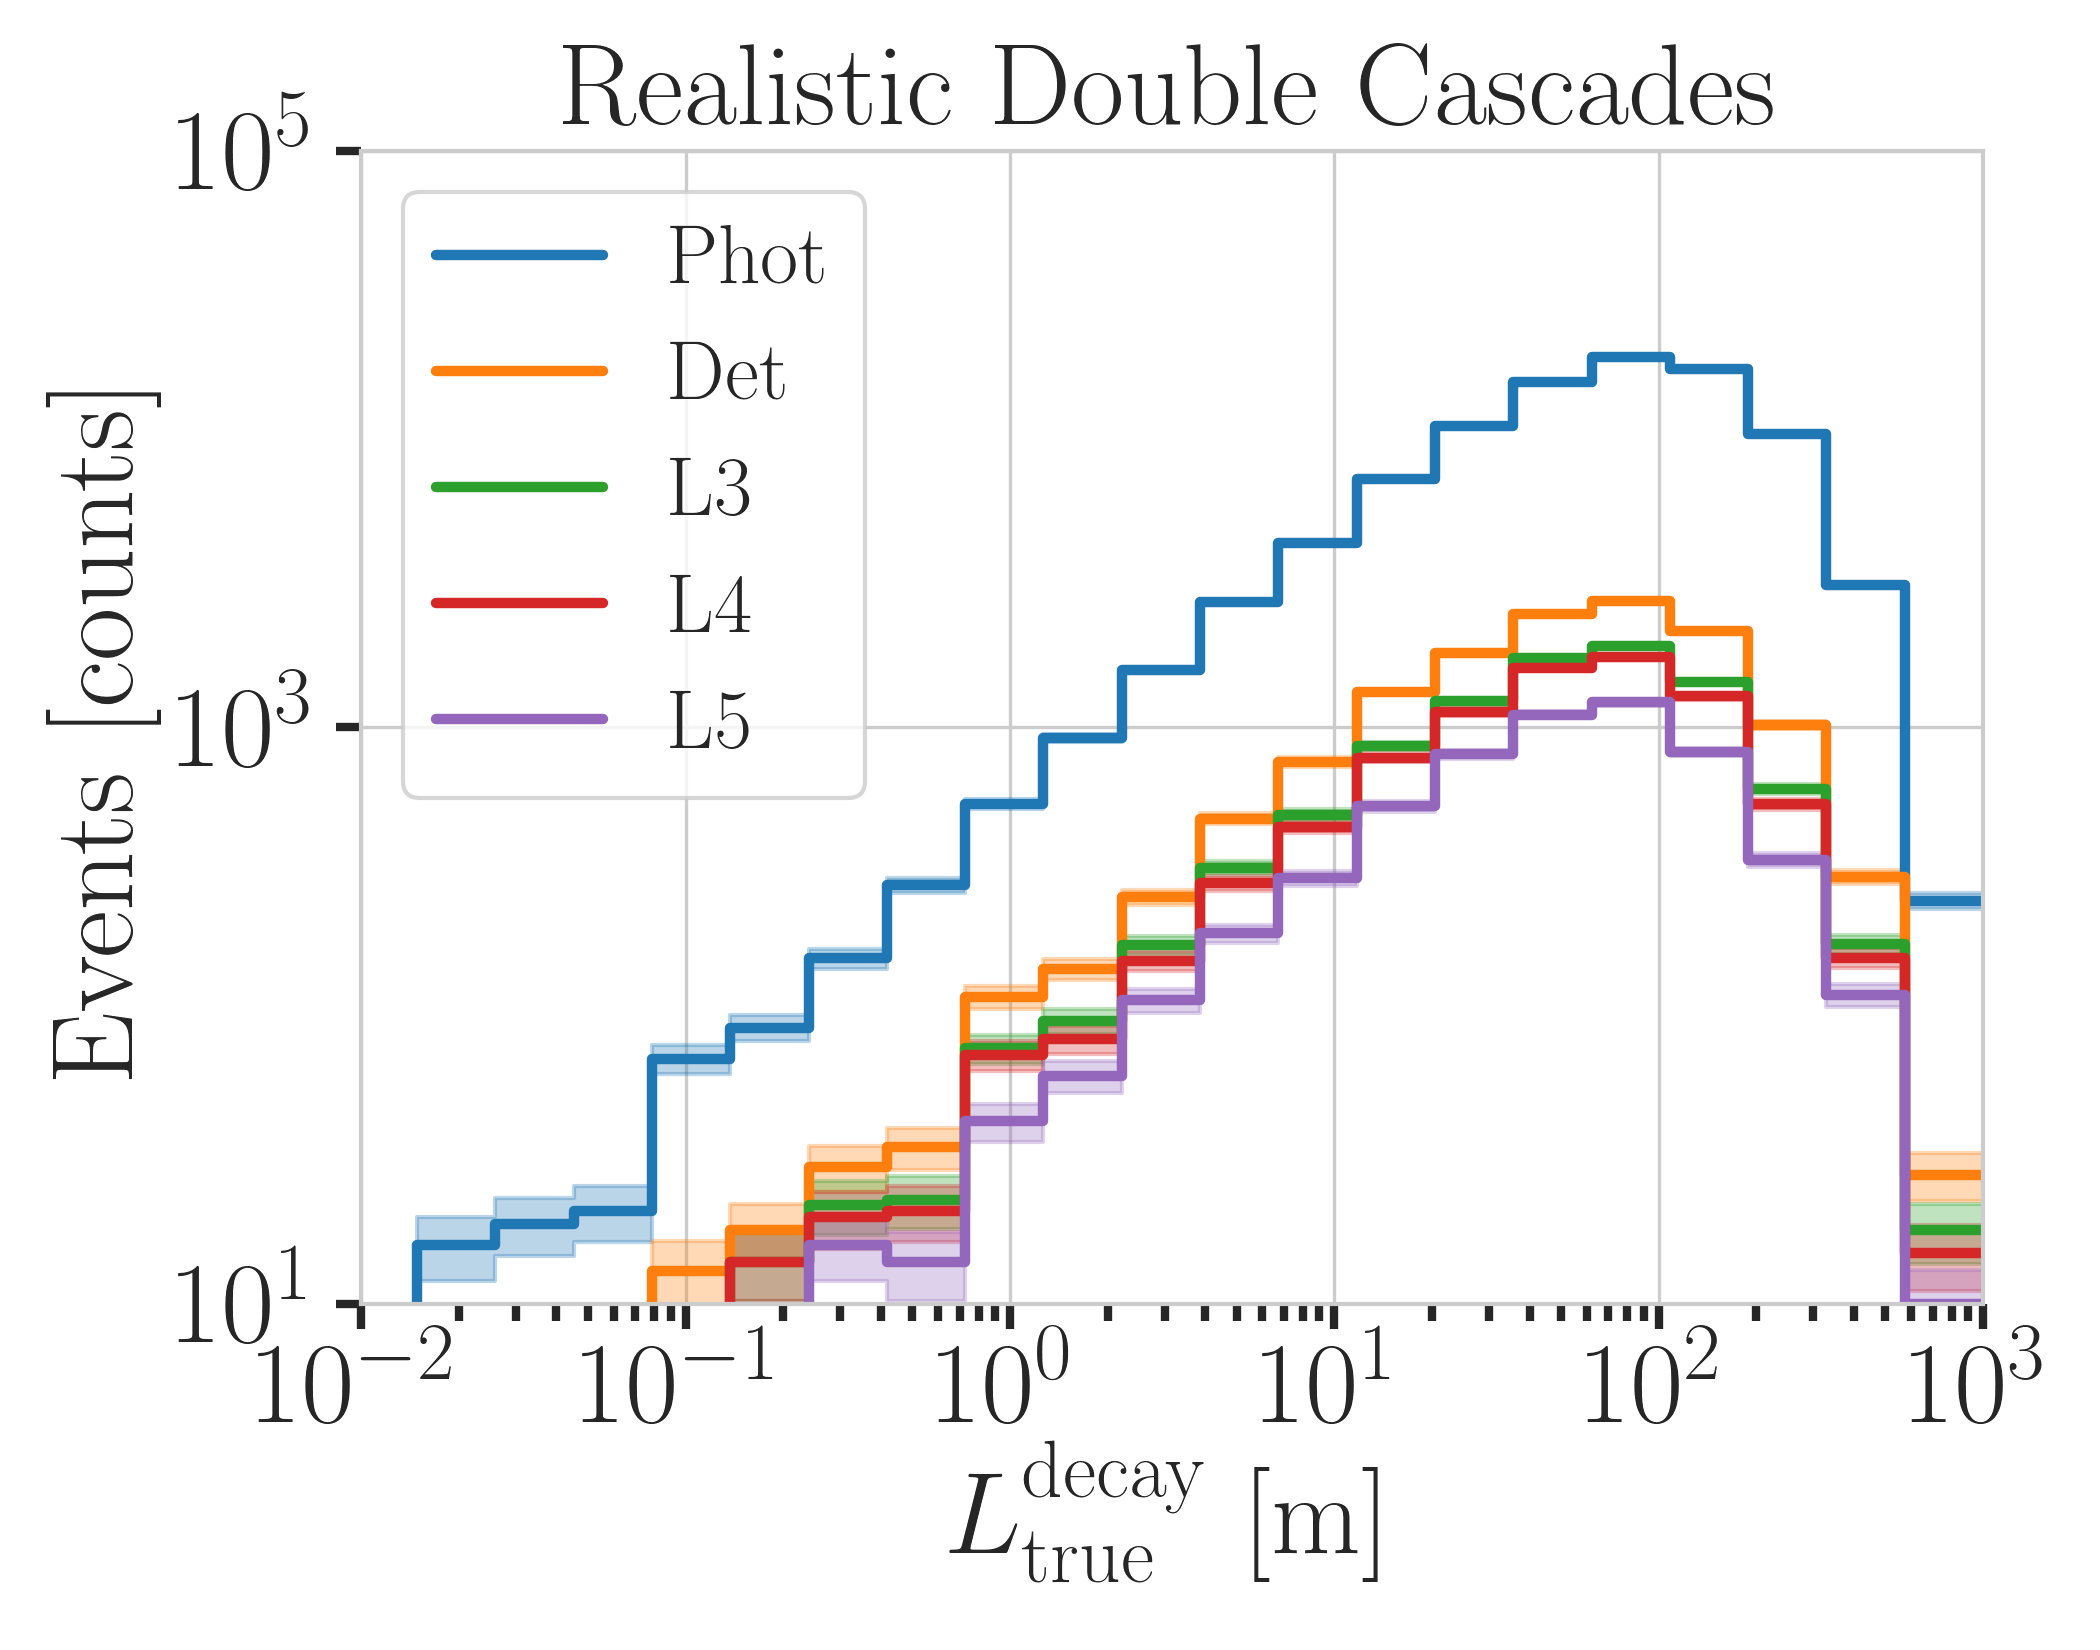
\includegraphics[width=0.49\linewidth]{figures/model_independent_simulation/results/realistic/selection/hnl_selection_efficiency_decay_l_true_unweighted.png}
    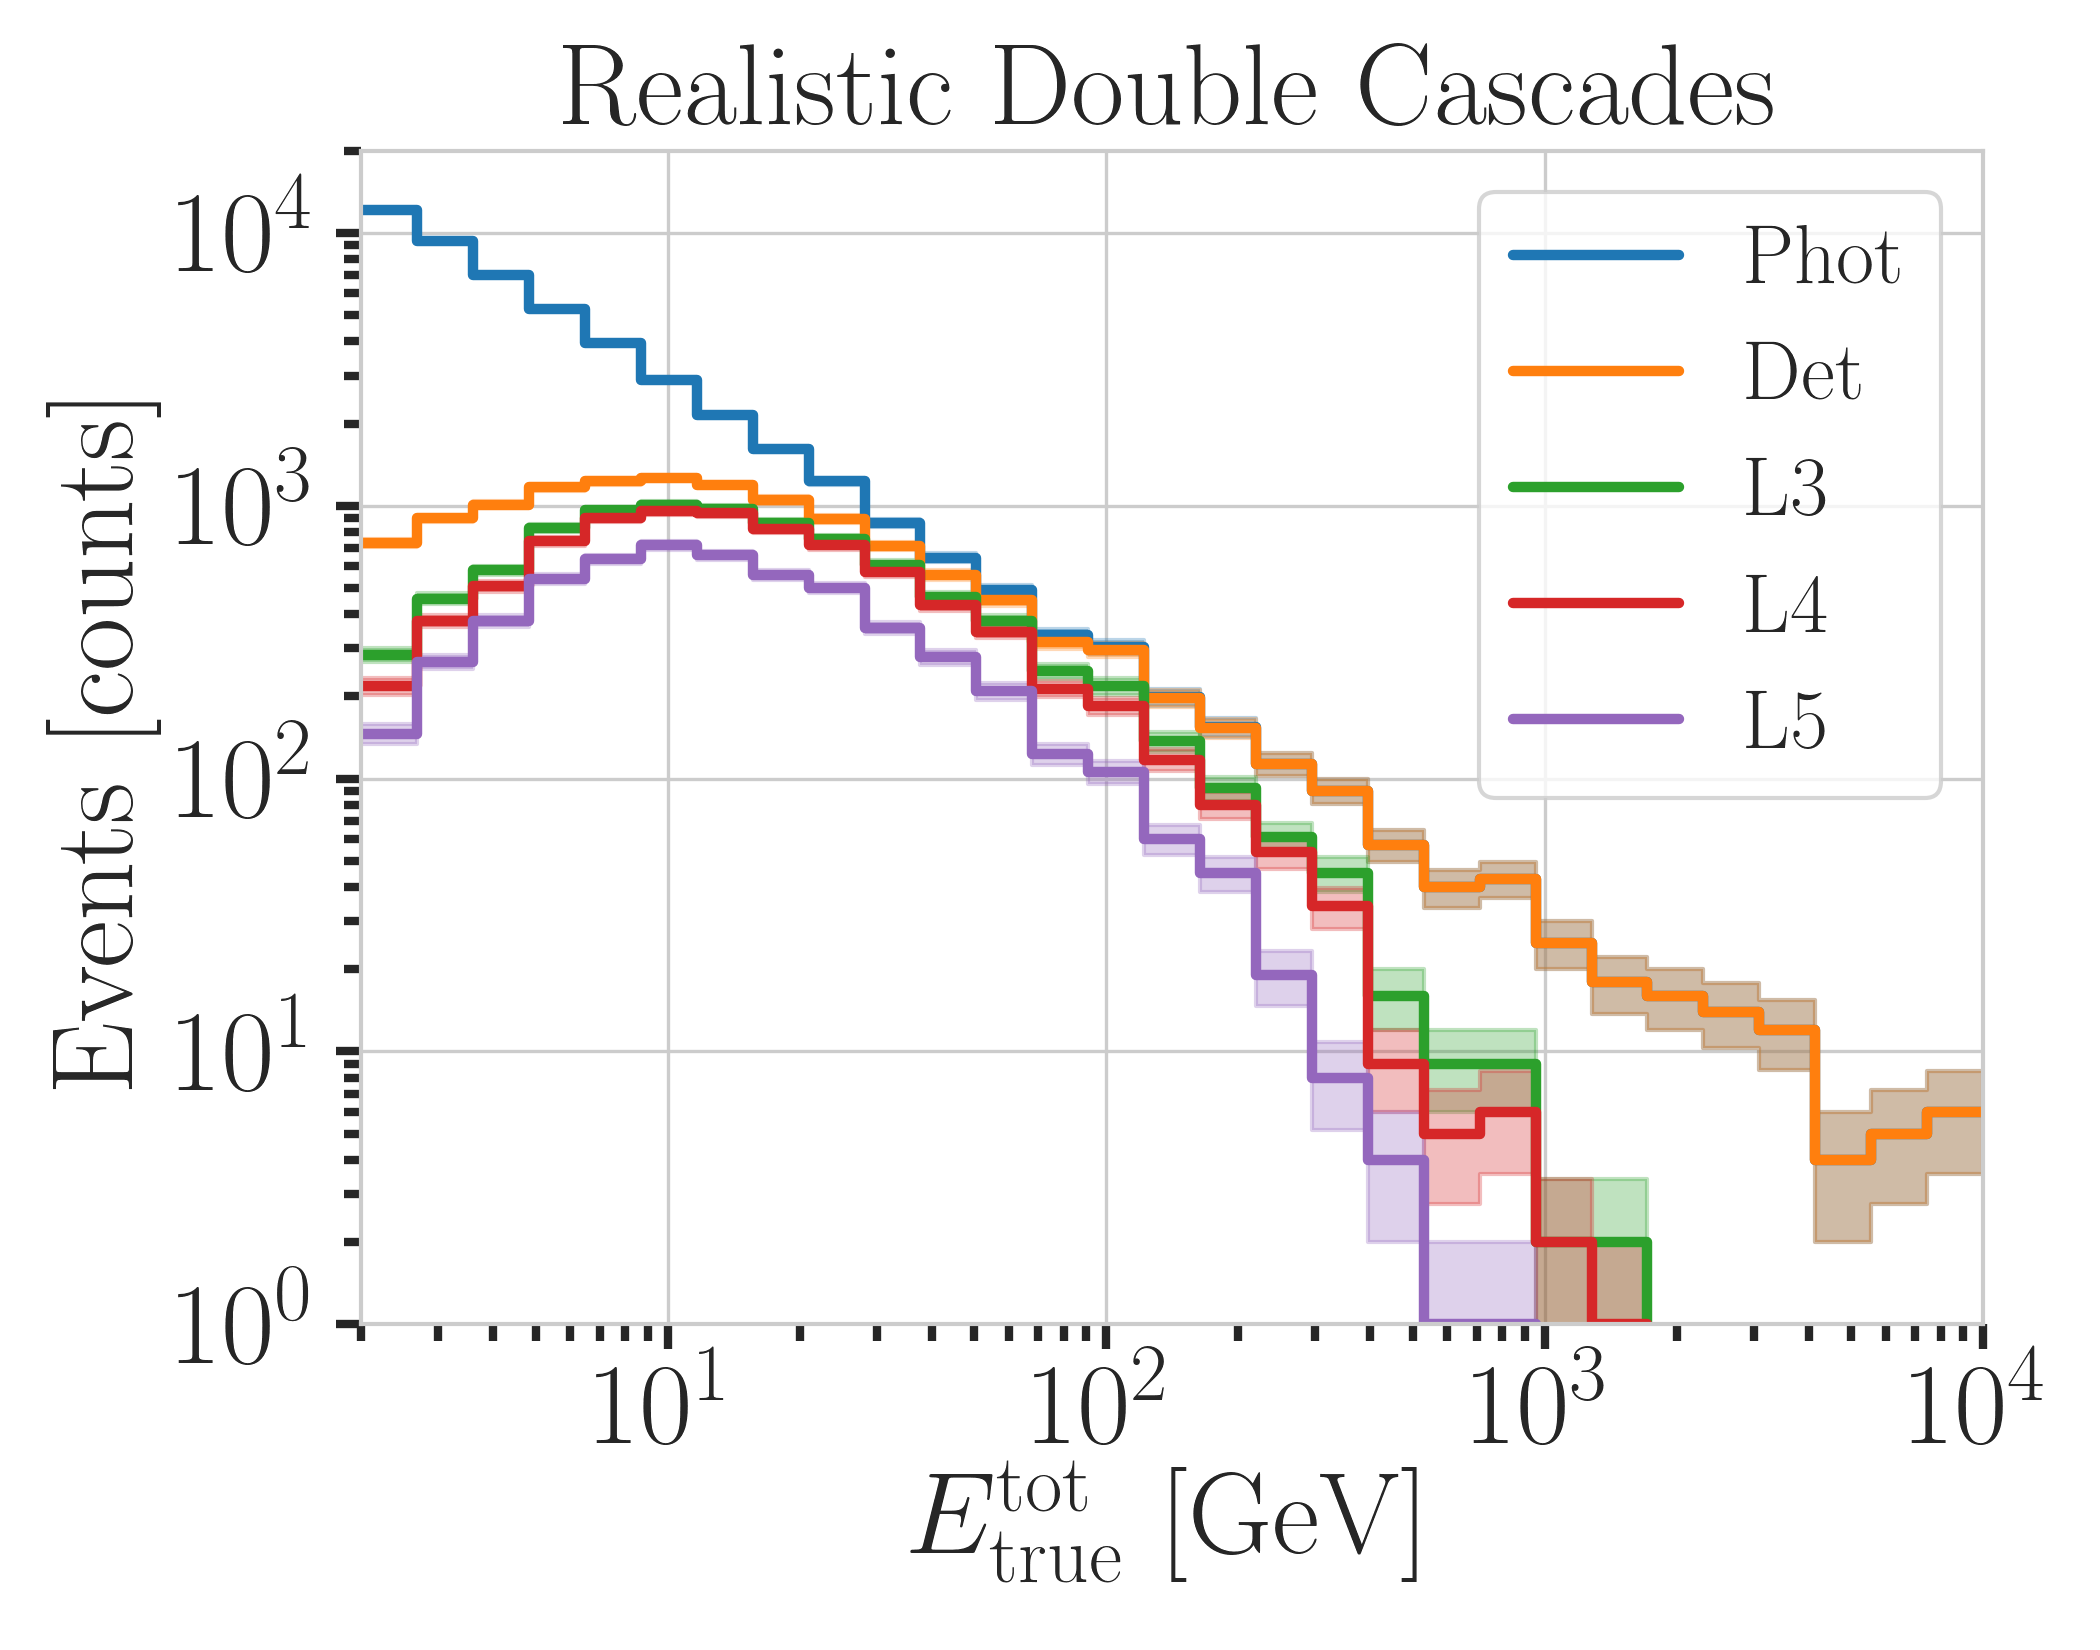
\includegraphics[width=0.49\linewidth]{figures/model_independent_simulation/results/realistic/selection/hnl_selection_efficiency_energy_true_unweighted.png}
    \caption[Realistic double-cascade selection efficiency]{Selection efficiency of the realistic  double-cascade sample. Shown is the true decay length distribution across the different selection levels (left) and the true energy distribution across the different selection levels (right).}
    \labfig{realistic_selection_efficiency}
\end{figure*}


\paragraph{Selection Efficiency:}

To assess the efficiency of the low-energy event selection for double-cascade events, the true energy and true decay length distributions are shown across the different selection levels in \reffig{realistic_selection_efficiency}. The two detector simulation steps explained in \refsec{detector_simulation} are also included, where the application of the detector response simulation (Det), reduces the events significantly at low energies, because only events with sufficient photons observed in the DOMs are kept. The L3 selection, which includes the DeepCore SMT-3 trigger, reduced both the low-energy region further, while also affecting the high-energy region. L4 and L5 reduce the overall number of events, without showing a specific energy dependence. The full selection appears to be independent of the true decay length, as the distributions reduces uniformly across the decay length range. Similar to the efficiency for SM neutrinos, the total selection efficiency from the online filter to L5 is around \SI{40}{\percent}.




\subsubsection{Model-Dependent Sample}

After optimizing the double-cascade reconstruction and benchmarking how it performs using the model-independent sample, the resolutions are investigated with the model-dependent HNL simulation. A preliminary sample of HNL events is used which contains masses between \SIrange[range-phrase=~and~]{0.1}{3.0}{\gev} and lab frame decay lengths in the range from \SIrange{1}{1000}{\meter}, sampled from an inverse distribution.

\begin{figure*}[h!]
	\centering
    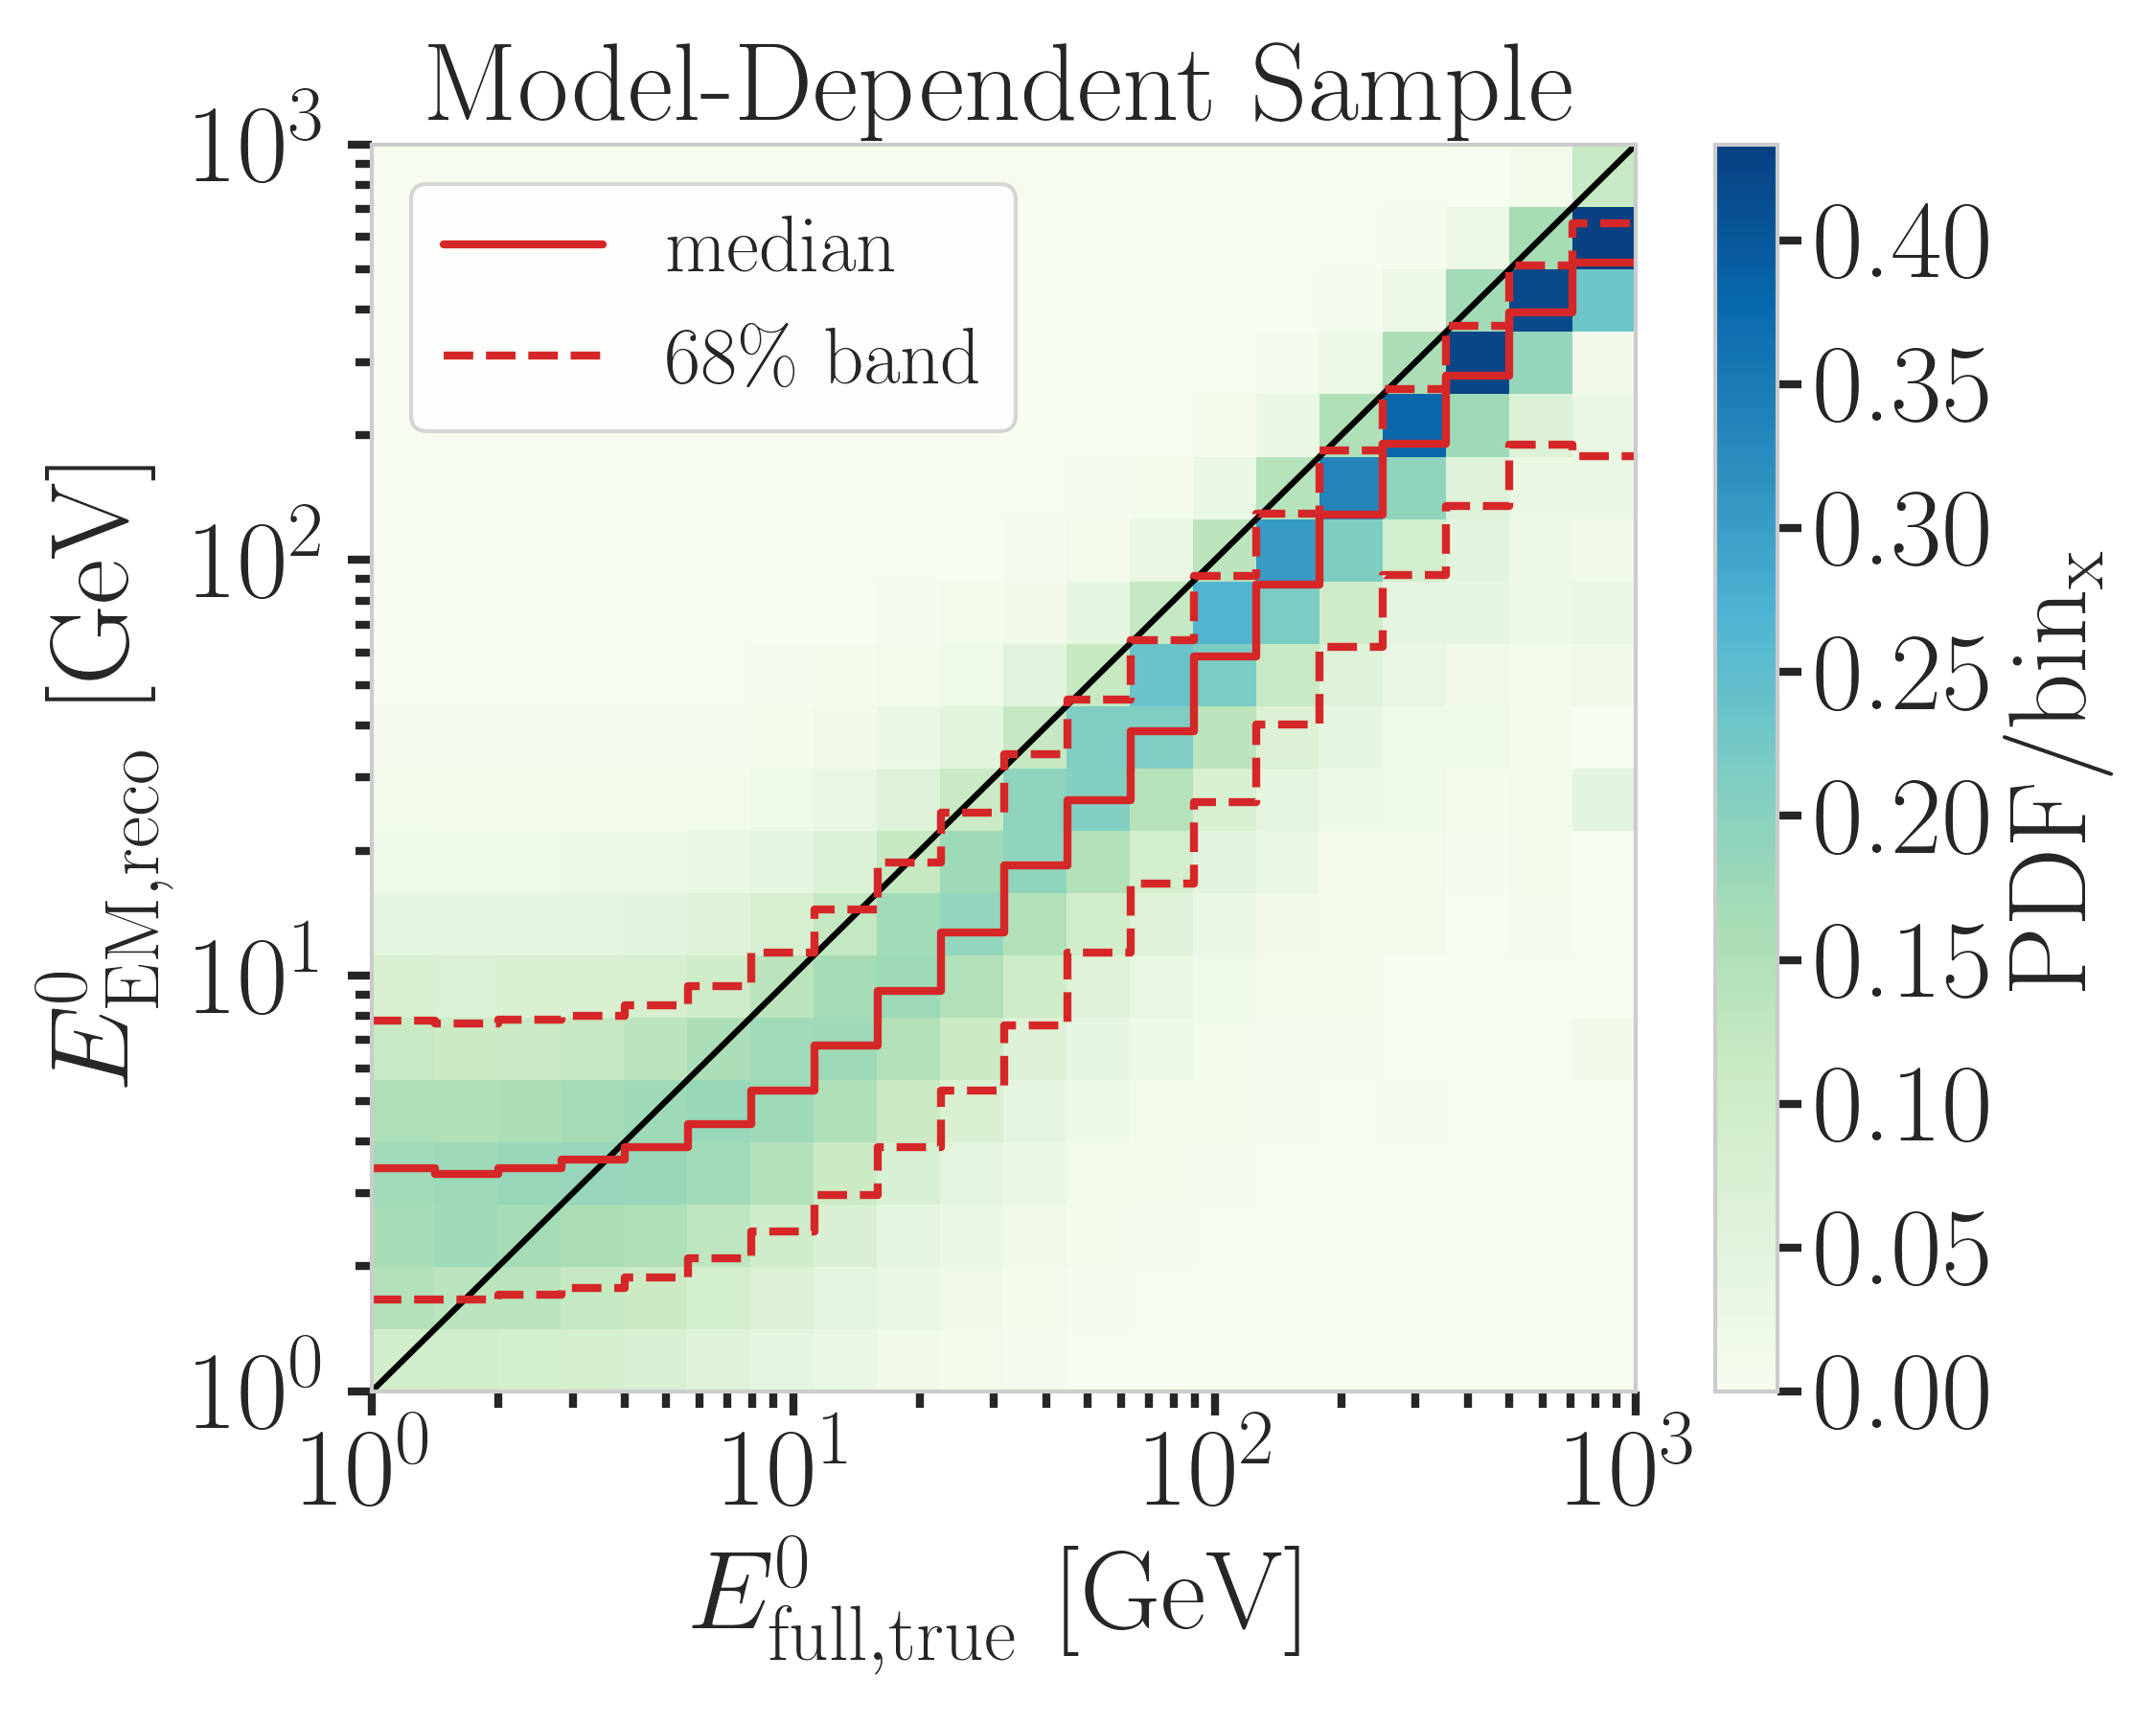
\includegraphics[width=0.49\linewidth]{figures/results/190607/resolutions/casc0_reco_energy_vs_casc0_true_energy_final_level_good_step_contours.png}
    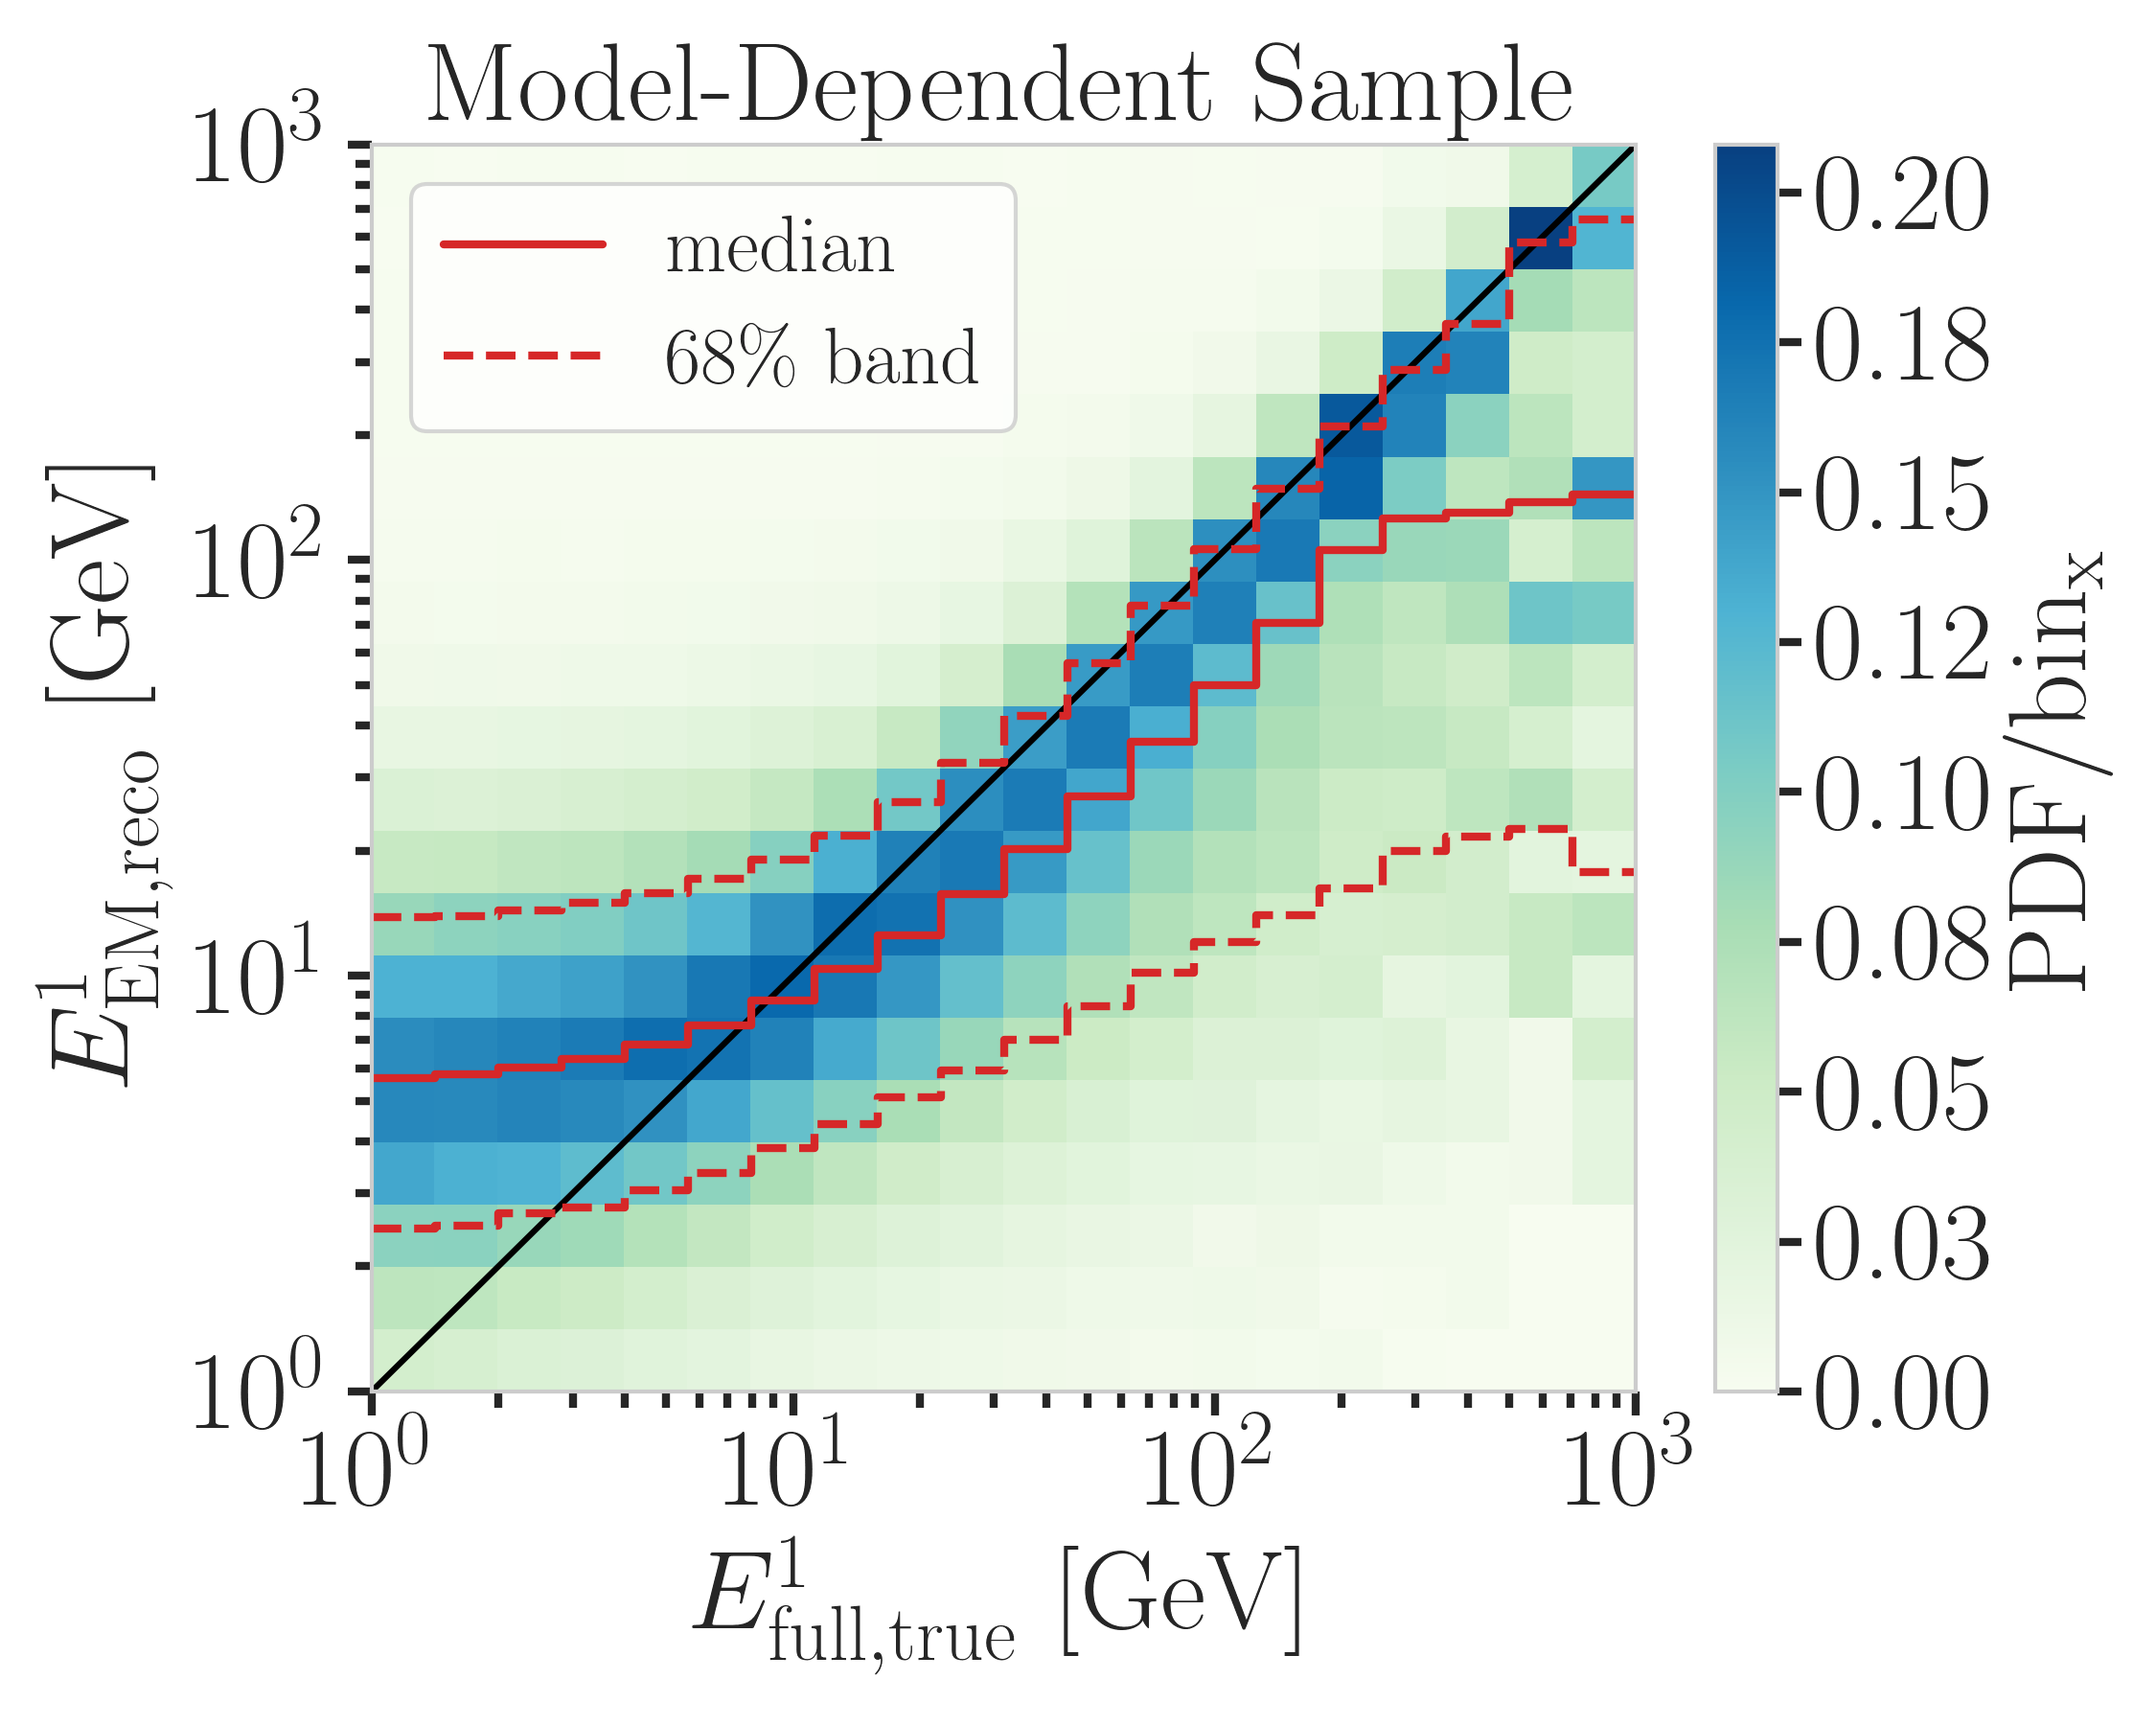
\includegraphics[width=0.49\linewidth]{figures/results/190607/resolutions/casc1_reco_energy_vs_casc1_true_energy_final_level_good_step_contours.png}
    \caption[Reconstructed cascade energies versus true energies - preliminary model-dependent sample]{Reconstructed (EM) energy versus true energy (full) energy for the first cascade (left) and second cascade (right) for a preliminary version of the model-dependent sample, where the color scale is normalized per vertical slice and the median and \SI{68}{\percent} band are shown in red.}
    \labfig{selected_routine_2d_energy_results}
\end{figure*}

The reconstructed energy versus the true energy is shown in \reffig{selected_routine_2d_energy_results}. The reconstructed energy is only the energy that was deposited as light in the detector. The true energies however, are the total cascade energies, including contributions that go into neutral particles that do not produce any light. It is therefore expected that the reconstructed energy is lower than the true and the median is offset with respect to the diagonal.

\begin{figure}[h]
    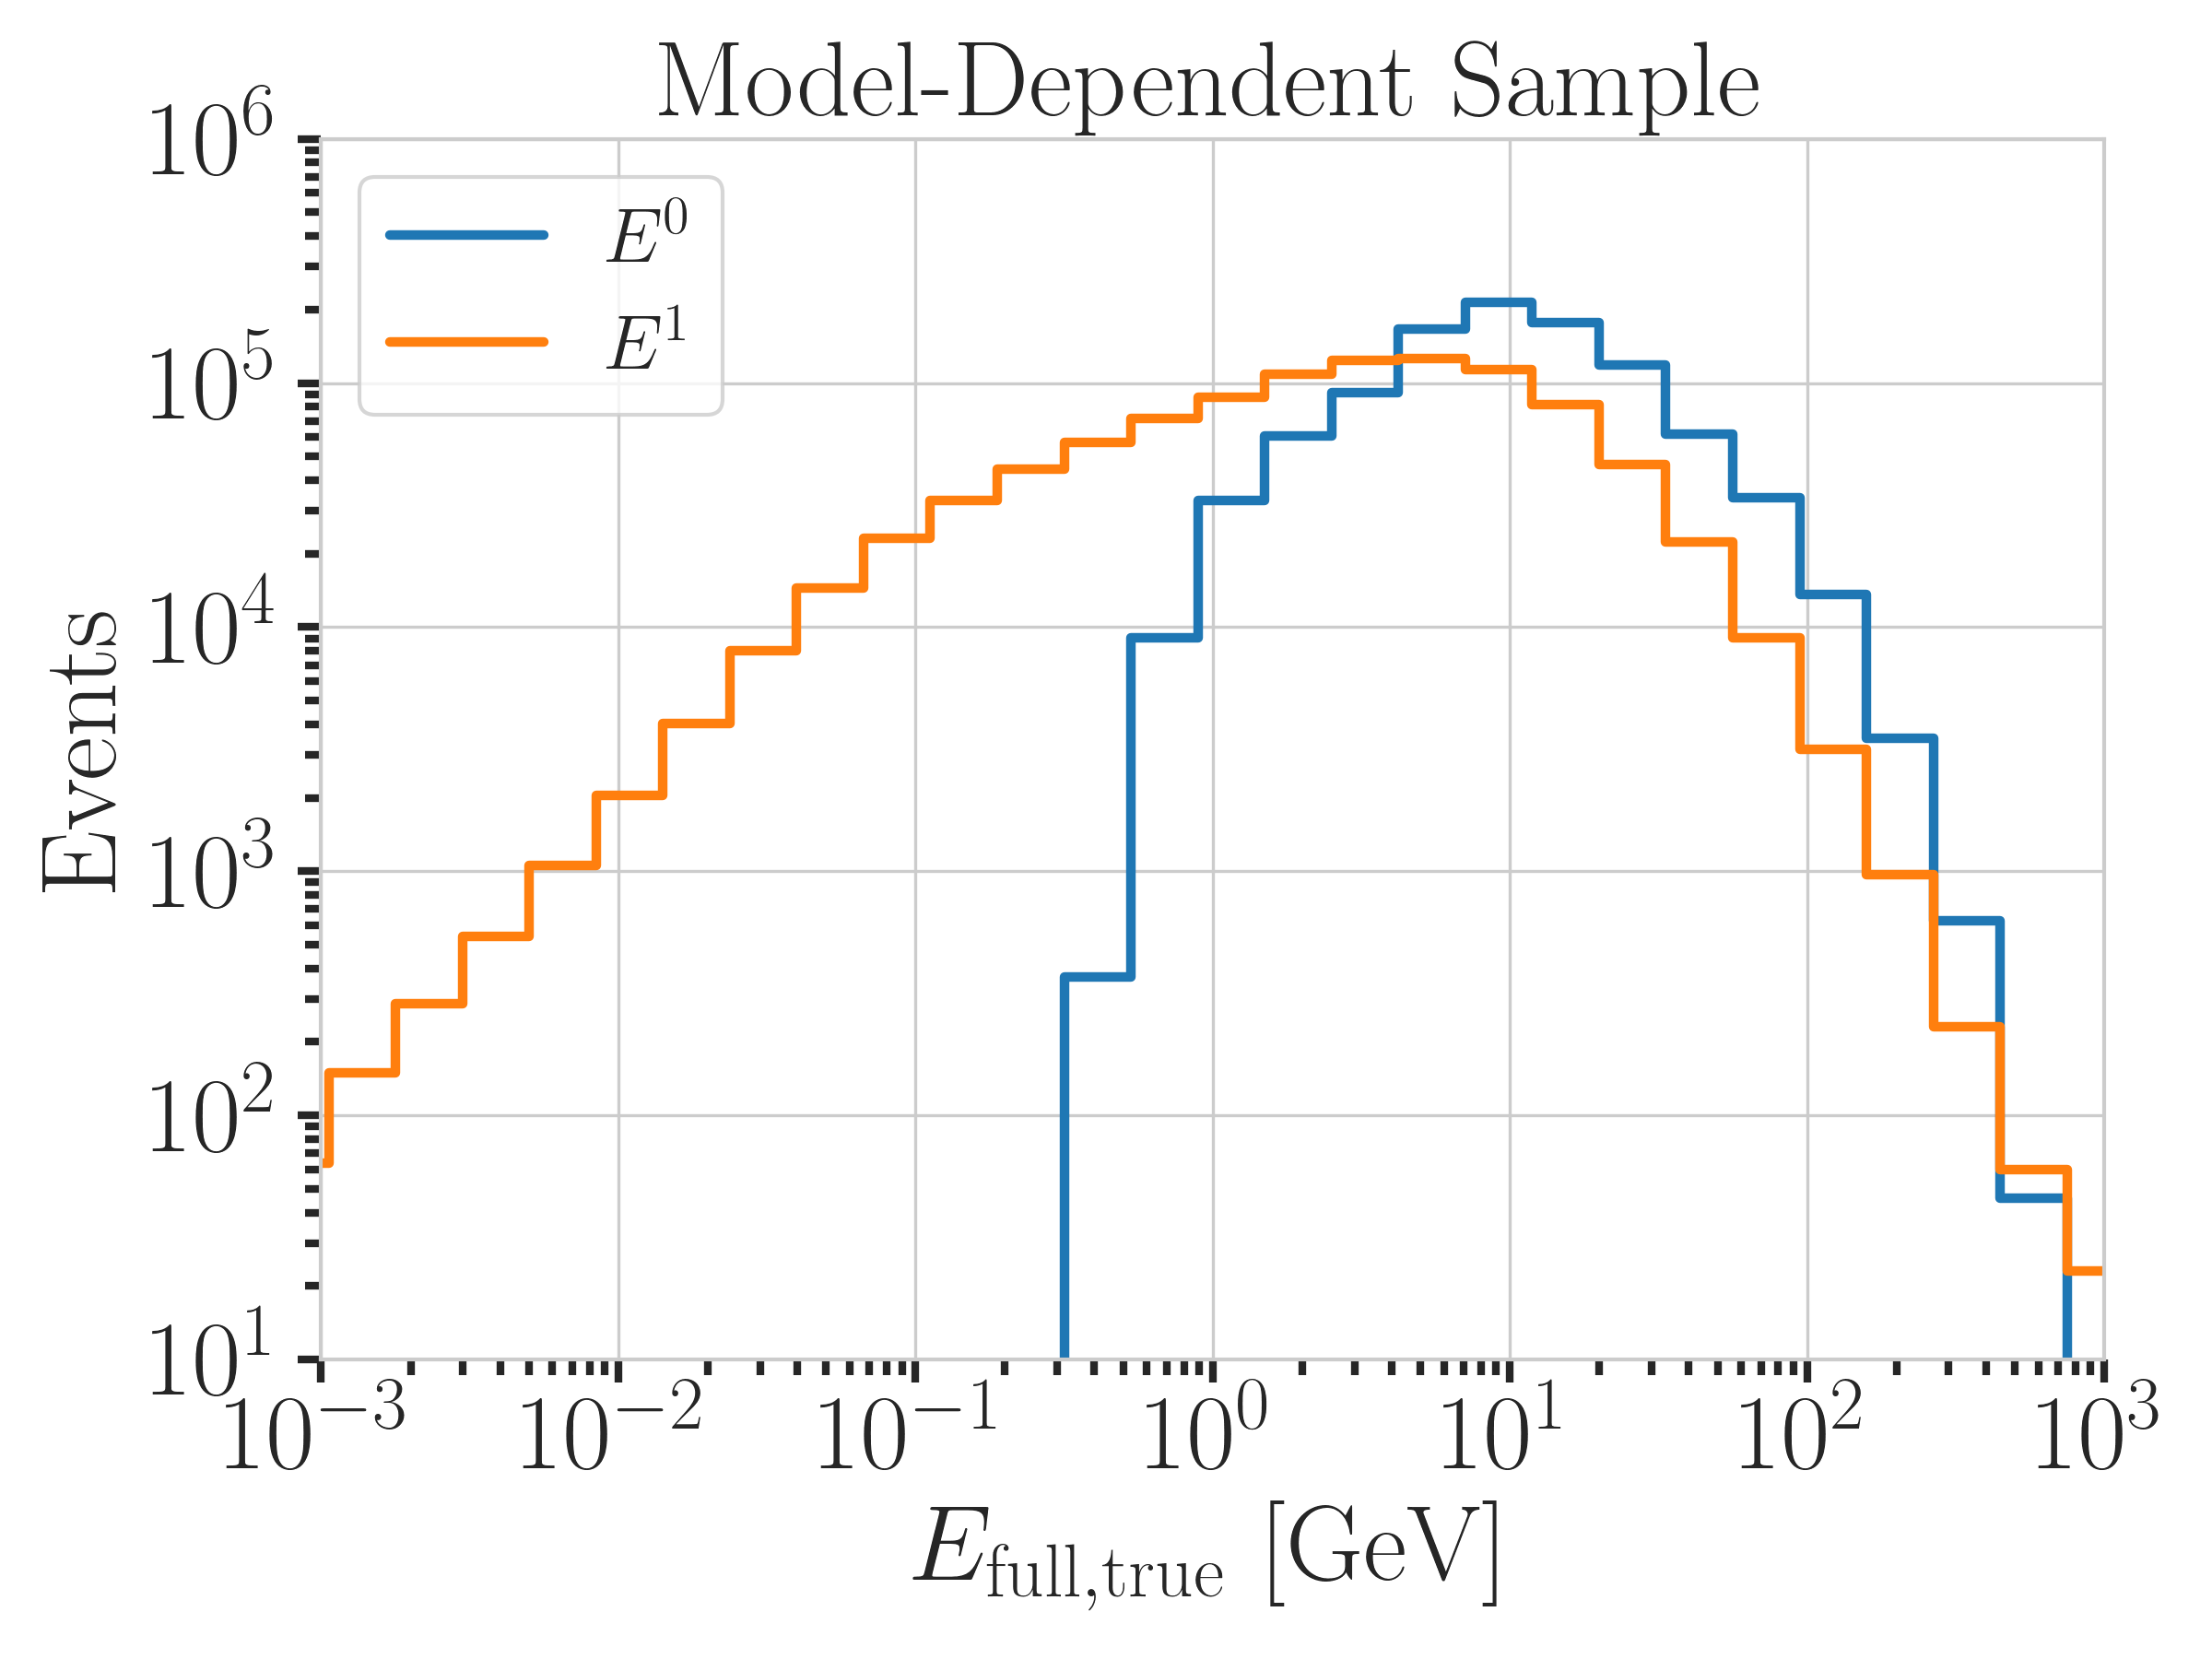
\includegraphics[width=0.8\textwidth]{figures/results/190607/190607_1_d_distr_cascades_final_level.png}
    \caption[True cascade energies - preliminary model-dependent sample]{True energy distributions of both cascades for a preliminary version of the model-dependent sample. The shown energies are the full energy of the cascades, including components that go into invisible particles.}
\labfig{190607_true_energies_final_level}
\end{figure}

Apart from this expected bias, the behavior is similar to the results observed for the realistic, model-independent sample shown in \reffig{cascade_energy_2dhists}. The performance appears to be worse for the second cascade, but for this sample, the energy distributions of the cascades are very different. Due to the kinematics of HNL production and decay introduced in \refsec{double_cascade_morphology}, the energy distribution of the second cascade is shifted to lower energies with respect to the energy distribution of the first cascade. \reffig{190607_true_energies_final_level} shows the energy distributions of both cascades for the same events shown in \reffig{selected_routine_2d_energy_results}. The energies of the first cascade peak around \SI{10}{\gev} and the lowest values are at the order of \SI{0.3}{\gev}, while for the second cascade, the peak of the distribution at $\sim$\SI{4}{\gev} and the lower end of the distribution extends multiple orders of magnitude below that. Note here, that these are again the true, total energies of the cascades, including the contributions that go into invisible particles. The true deposited energies are therefore lower.

\begin{figure}[h!]
    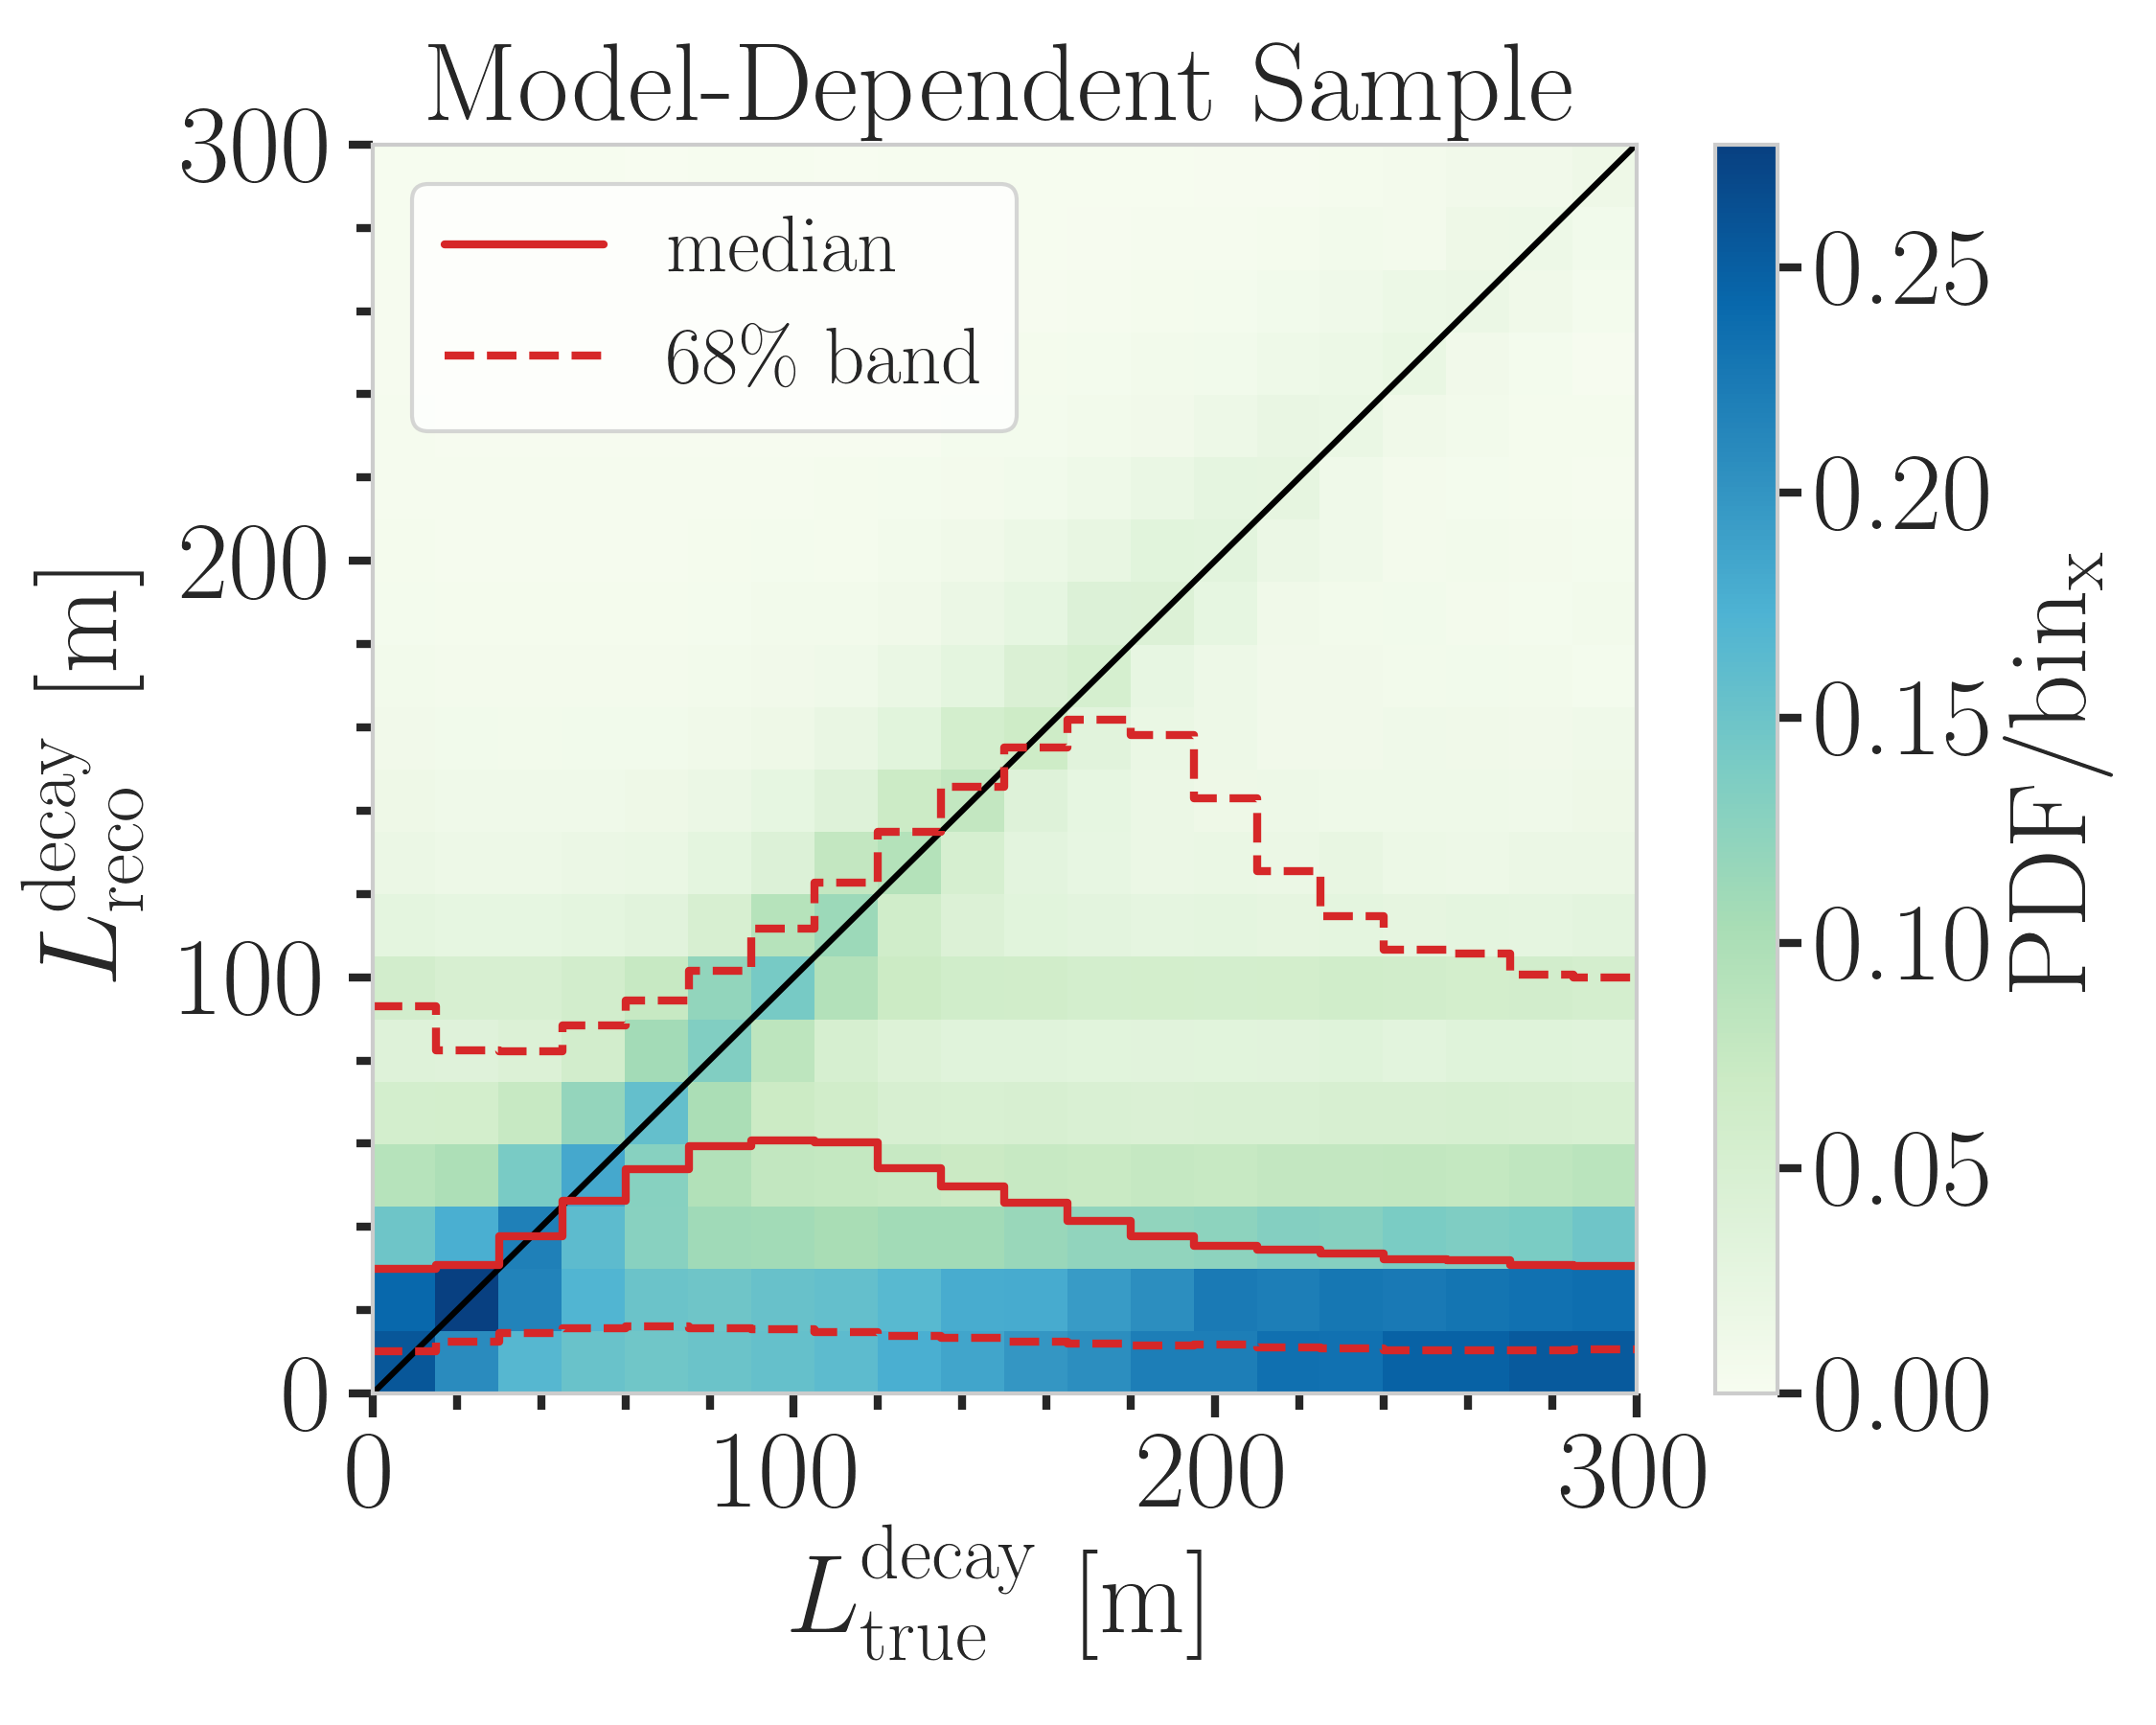
\includegraphics[width=0.8\textwidth]{figures/results/190607/resolutions/reco_decayL_vs_true_decayL_final_level_good_step_contours.png}
    \caption[Reconstructed decay length resolution versus true decay length - preliminary model-dependent sample]{Reconstructed decay length versus true decay length for a preliminary version of the model-dependent sample, where the color scale is normalized per vertical slice and the median and \SI{68}{\percent} band are shown in red.}
\labfig{190607_reco_decay_l_vs_true_decay_l}
\end{figure}
The reconstructed decay length versus the true decay length is shown in \reffig{190607_reco_decay_l_vs_true_decay_l}. The same behavior as observed for the realistic, model-independent sample shown in \reffig{realistic_sample_decay_length_2dhists} is seen. For short true decay lengths the reconstruction is over-estimating the length, while for long true decay lengths the reconstruction is strongly under-estimating the length and a population of badly reconstructed events is dominating at long true decay lengths.


\subsubsection{Summary and Outlook}

A double-cascade reconstruction was optimized for low-energy HNL events inside the DeepCore volume. A thorough investigation of the performance revealed a number of difficulties in reconstructing these events. The most challenging cause is the low light yield. For the simulation using physically accurate models, this was especially bad, because part of the event's energy goes into neutral particles, which produce no light in the detector. From the investigation of the double-cascade reconstruction performance, it can be concluded that the main reason for the bad reconstruction is the low-energy of the second cascade. Other factors, like the position of the cascades in less densely instrumented regions of the detector also contribute at a lower level.

It may be possible to improve the performance through more sophisticated reconstruction techniques. Also, the reduced spacing and segmented directionality of optical modules in the future IceCube Upgrade detector should enhance the light detection of low-energy cascades and should yield a better chance to identify the unique HNL signature. Data taking for this new low-energy extension is expected to begin in 2026.


\section{Double-Cascade Classification} \labsec{dc_classification}

Despite the failure of the reconstruction for events with low energy depositions, there is still a population of well reconstructed events. The next step is to see how well these can be distinguished from the SM backgrounds. For this purpose a classifier was trained to distinguish between HNL \textit{signal} events and SM neutrino \textit{background} events. To mitigate the poorly reconstructed events, a selection was applied to make sure the classifier is trained on well reconstructed events. The selection criteria require a minimum reconstructed energy of both cascades of \SI{5}{\gev} and a minimum reconstructed decay length of \SI{40}{\meter}. The same criteria are applied to both signal and background events.

\begin{figure}[h]
    \centering
    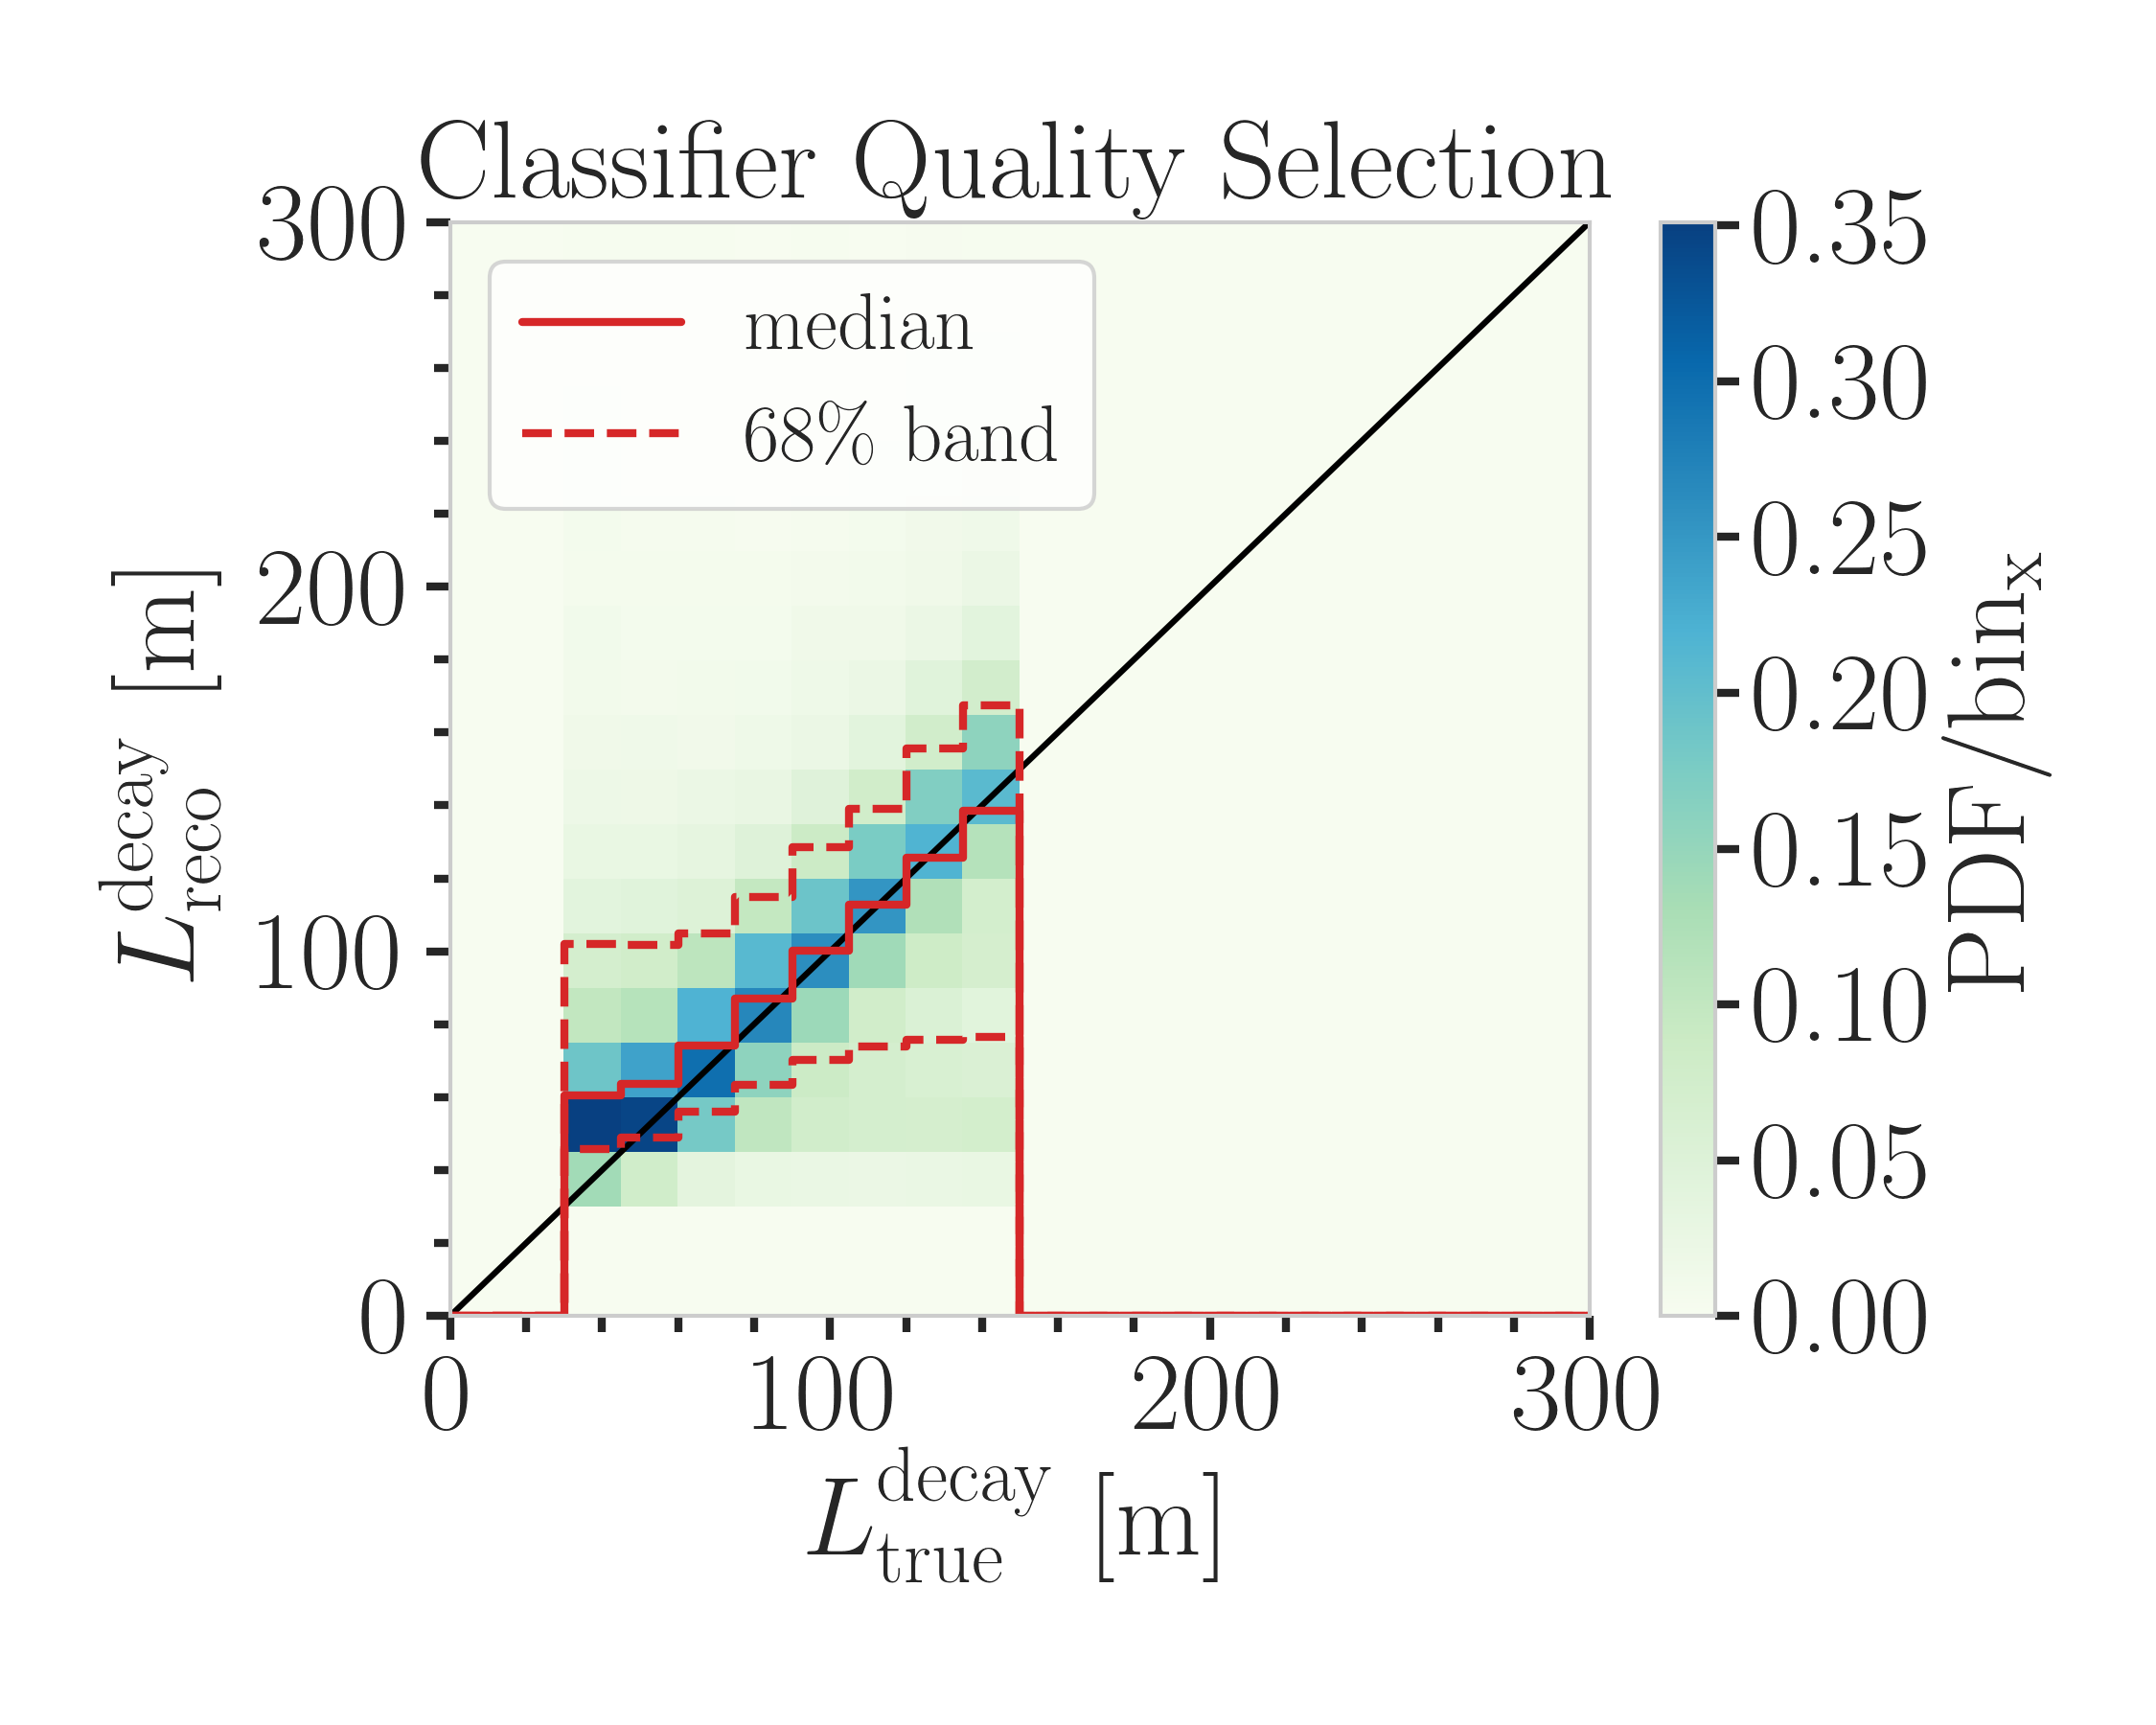
\includegraphics[width=0.8\textwidth]{figures/results/190607/classification/reco_decayL_vs_true_decayL_reco_energy_cut_and_reco_length_cut_and_true_energy_cut_and_true_length_cut_step_contours.png}
    \caption[Reconstructed decay length resolution versus true decay length after quality selection - preliminary model-dependent sample]{Reconstructed decay length versus true decay length for a preliminary version of the model-dependent sample, after the quality selection was applied. The color scale is normalized per vertical slice and the median and \SI{68}{\percent} band are shown in red.}
    \labfig{classifier_cuts_length_2d_hist}
\end{figure}

Additionally, some requirements on the true energies and decay length were applied for the signal, which are a minimum true energy of both cascades of \SI{5}{\gev}, and a true decay length between \SIrange[range-phrase={~and~}]{40}{150}{\meter}. These were chosen to make sure the HNL events were theoretically double-cascade-like and at a sensible length scale inside DeepCore. \reffig{classifier_cuts_length_2d_hist} shows the reconstructed decay length versus the true decay length after the selection was applied.

The classifier used was a BDT from the \textit{\textsc{scikit-learn} (sklearn)} package~\sidecite{sklearn} and the input features are taken from the double-cascade reconstruction explained in \refsec{dc_reconstruction} as well as some additional variables from earlier levels of the processing explained in \refsec{processing_chain}. \reffig{example_BDT_features} shows the distributions of two example input features, where the left plot shows the output probability of the classifier trained to distinguish track from single-cascade-like events, which is used in the oscillation analysis, and the right plot shows the reconstructed decay length from the double-cascade reconstruction. Shown are the distributions for the signal, the individual track and cascade background components, and the total background. The distributions are normalized to the same area to show their shapes and it can be seen that the signal and total background distributions look very similar, while there is some differences to the background split in track and single-cascade component. For completeness, the selected features and their importances for the results presented in the following are shown in \refsec{dc_classifier_features_appendix}.

\begin{figure*}[h]
	\centering
    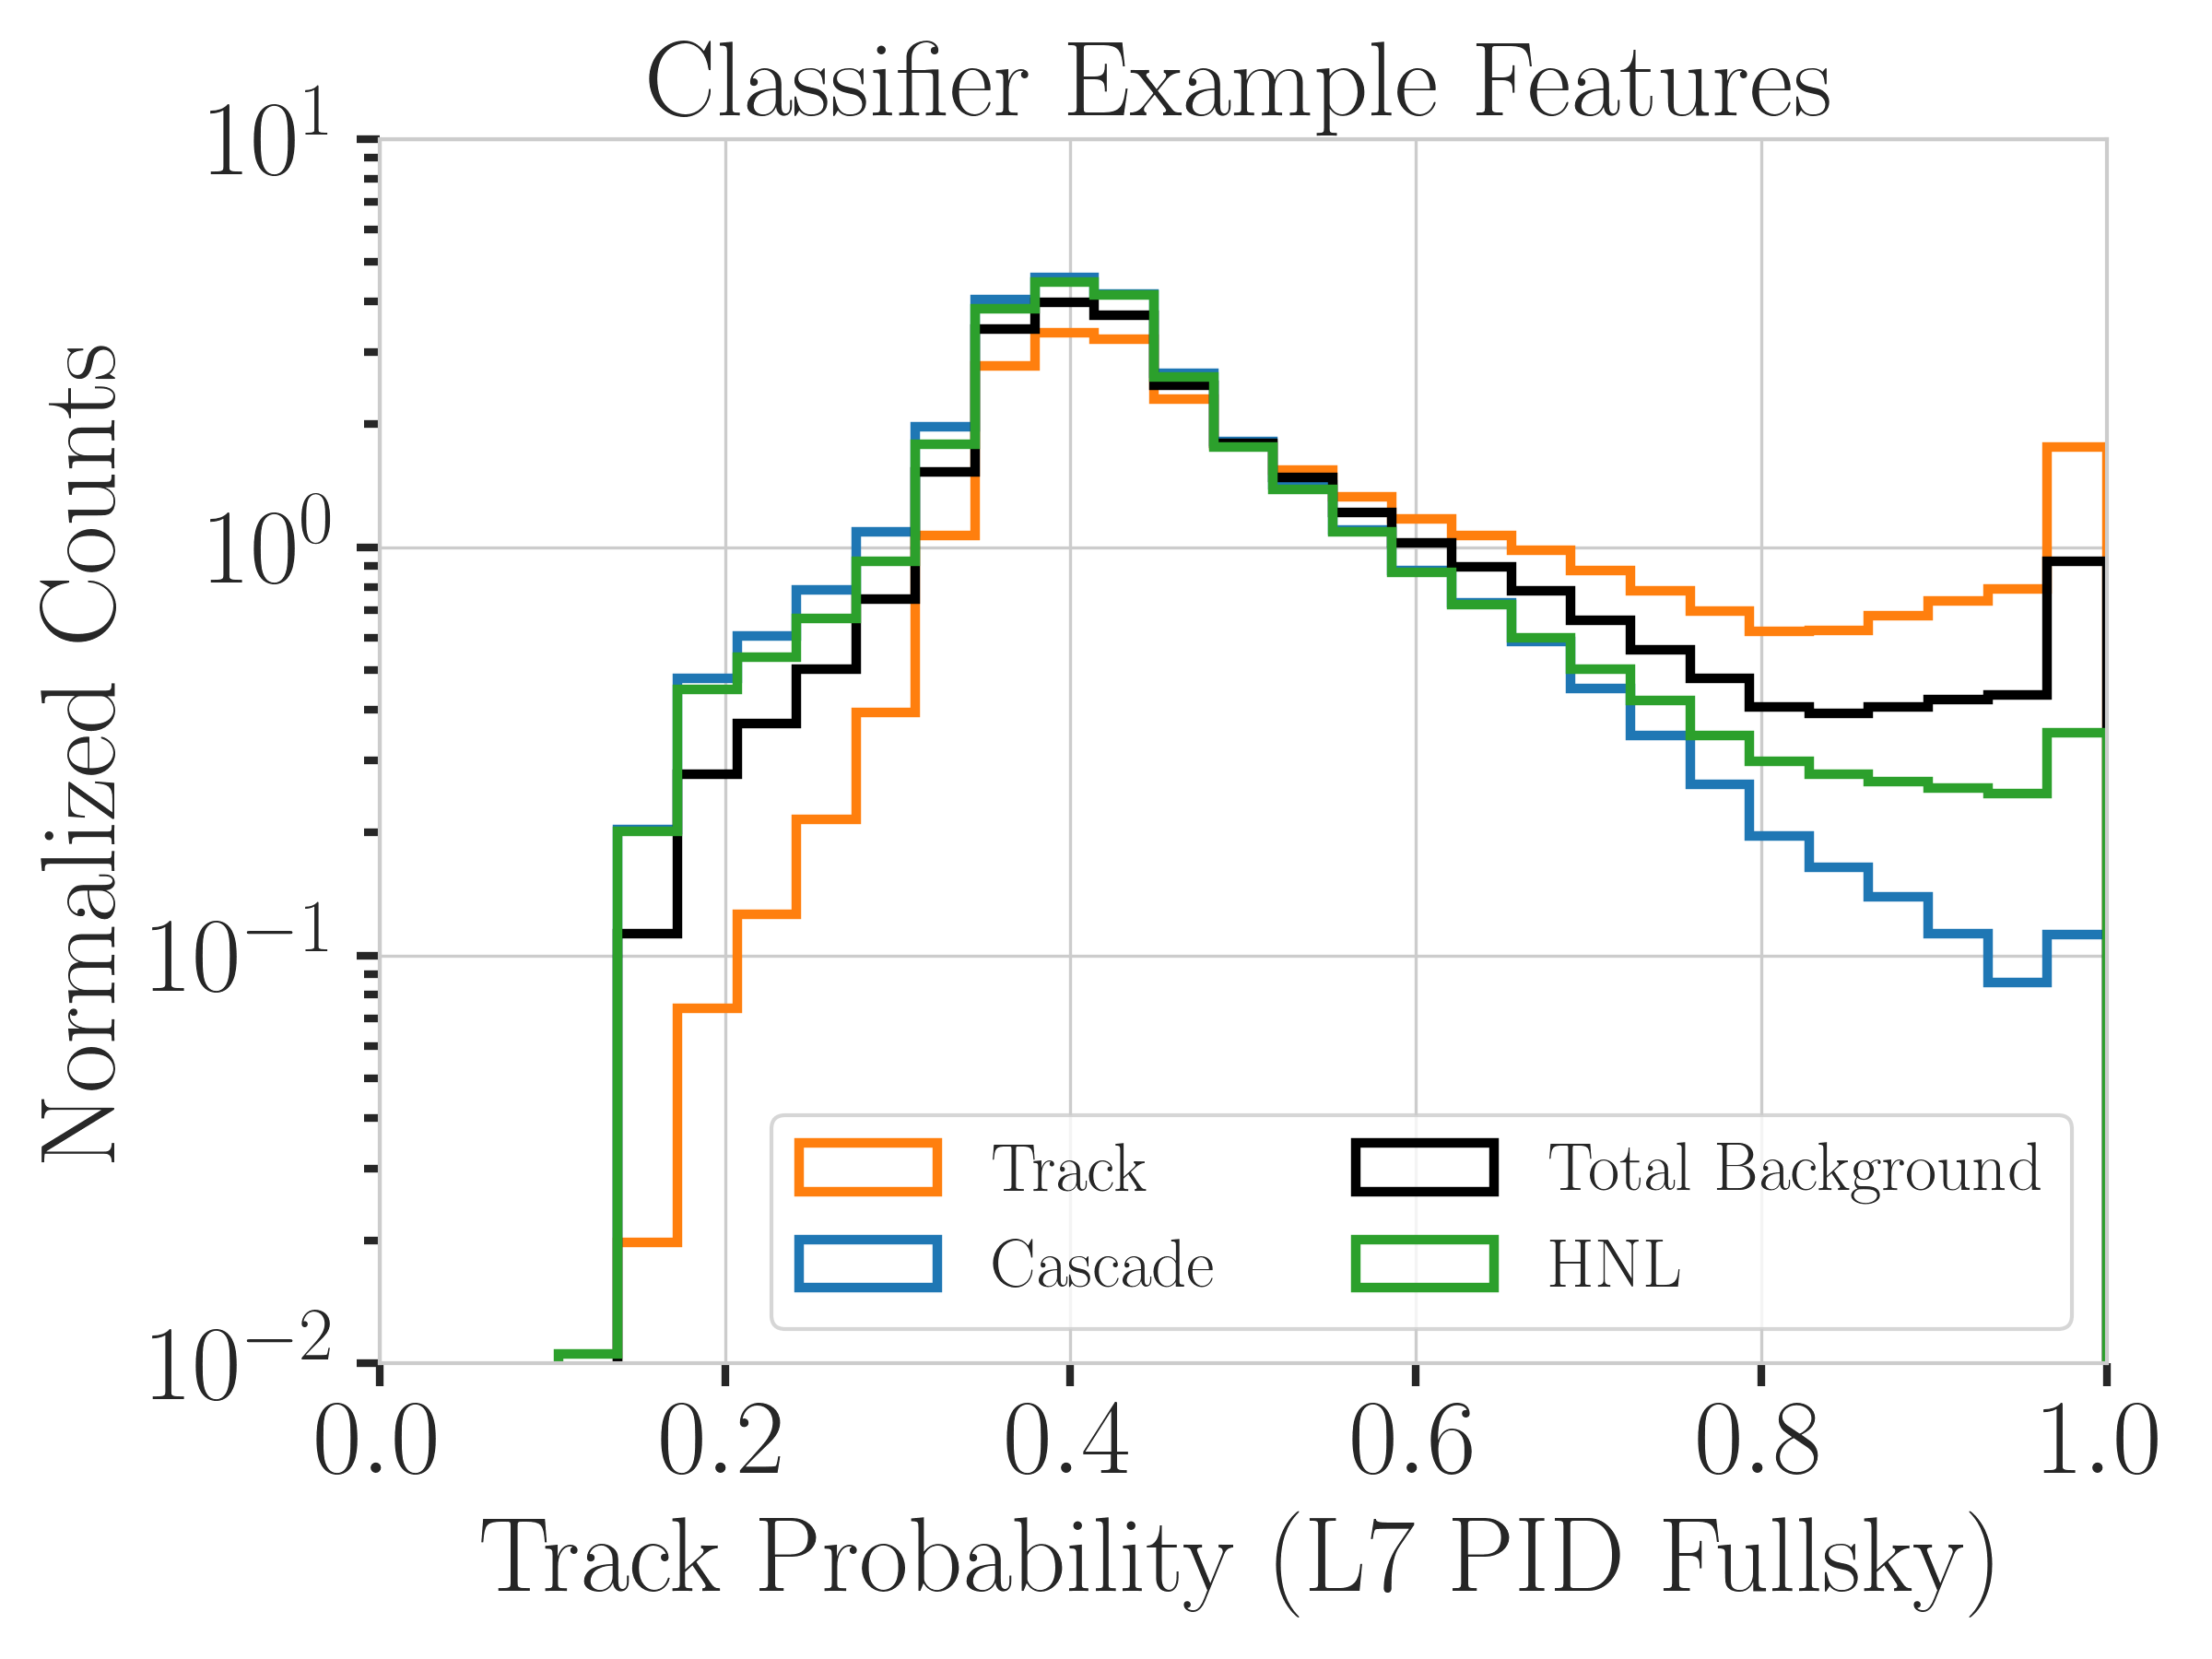
\includegraphics[width=0.49\linewidth]{figures/results/190607/classification/1_d_distr_L7_PIDClassifier_FullSky_ProbTrack_unweighted.png}
    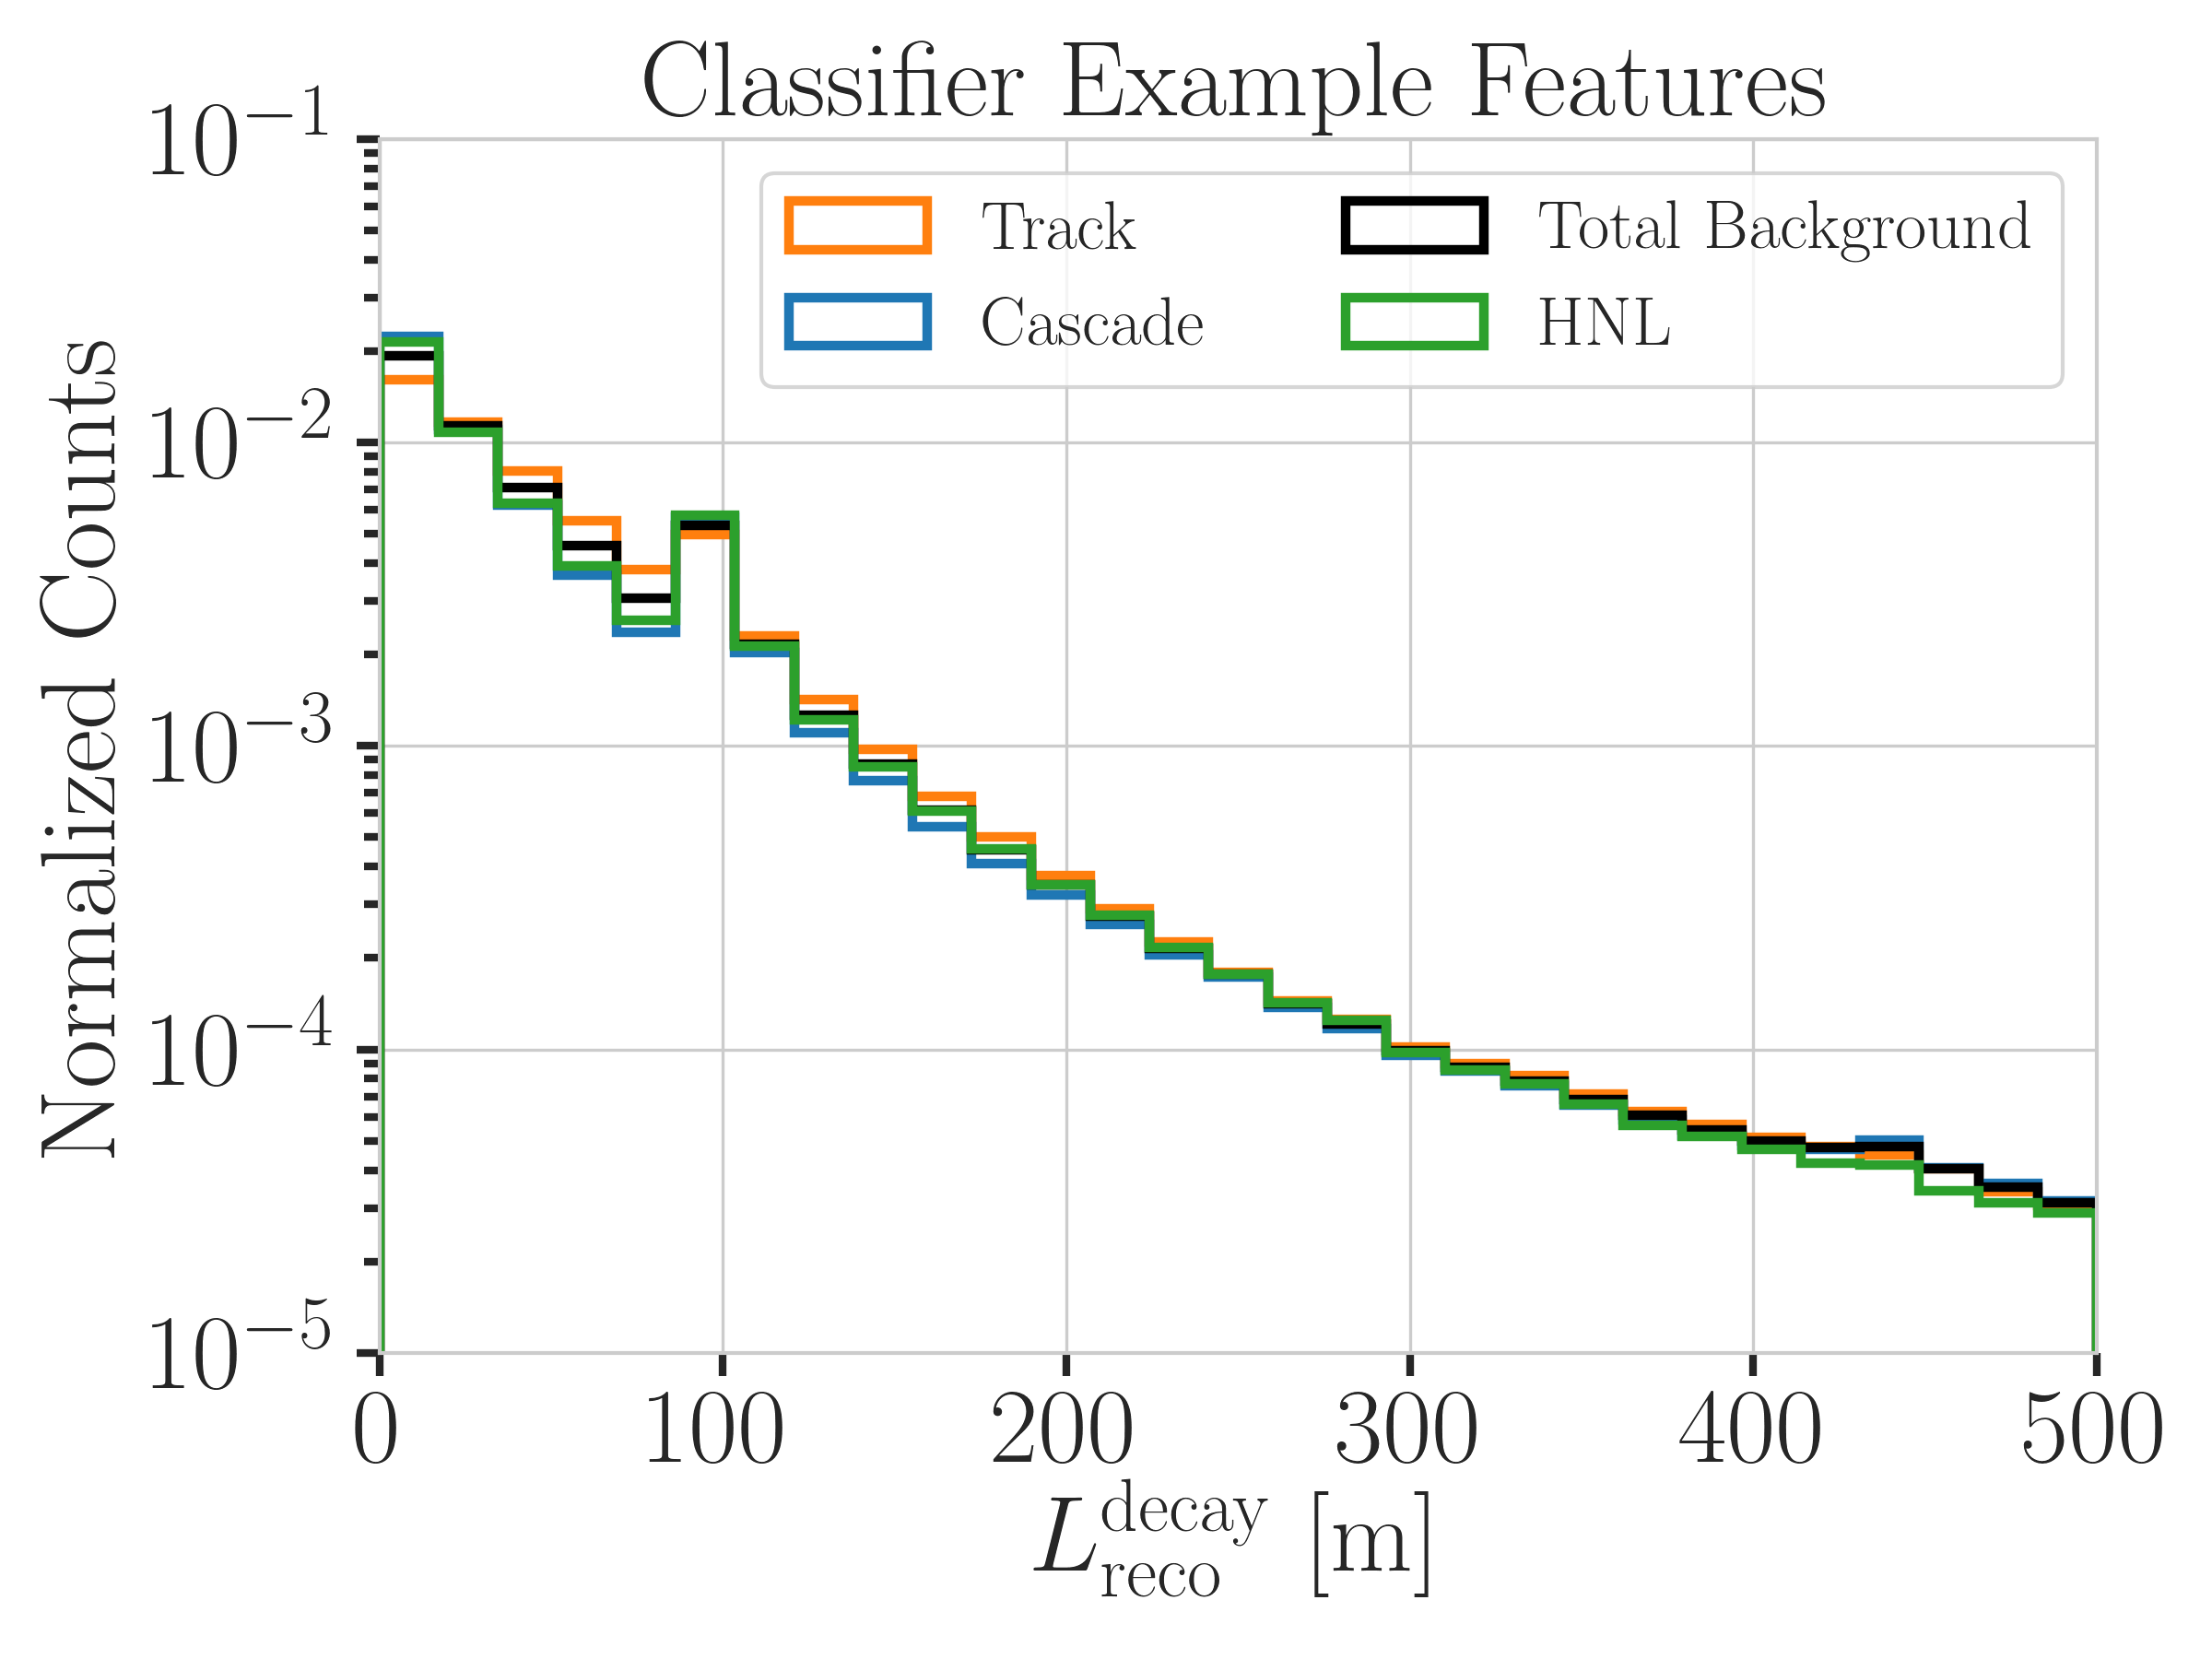
\includegraphics[width=0.49\linewidth]{figures/results/190607/classification/1_d_distr_reco_decayL_unweighted.png}
    \caption[Double-cascade classification example features]{Example features used for the double-cascade classification. Shown is the output probability of the classifier trained to distinguish track from cascade-like events (left) and the reconstructed decay length from the double-cascade reconstruction (right) for the different background signatures, the total background, and the signal. Distributions are normalized to.}
    \labfig{example_BDT_features}
\end{figure*}

A \textit{single-classifier} and \textit{double-classifier} approach were tested. For the single-classifier, one BDT classifier was trained to distinguish between signal events and all background events at once. For the double-classifier, two classifiers were trained separately, one to distinguish signal from track-like background, and the other to distinguish signal from cascade-like background. The classifiers were trained with uniform weights, but scaled so that the summed weights for signal and background were equal. Since the SM neutrino events at these energies are either track-like or cascade-like, the double-classifier approach performed better and will be discussed here. Despite the fact that several combinations of features were tested, it was not possible to identify a pure double-cascade region with a single classifier. Since the results did not show a strong classification power, tuning the hyperparameters quickly lead to overtraining and the results here are using the default settings of the BDT classifier.


\begin{figure*}[h]
	\centering
    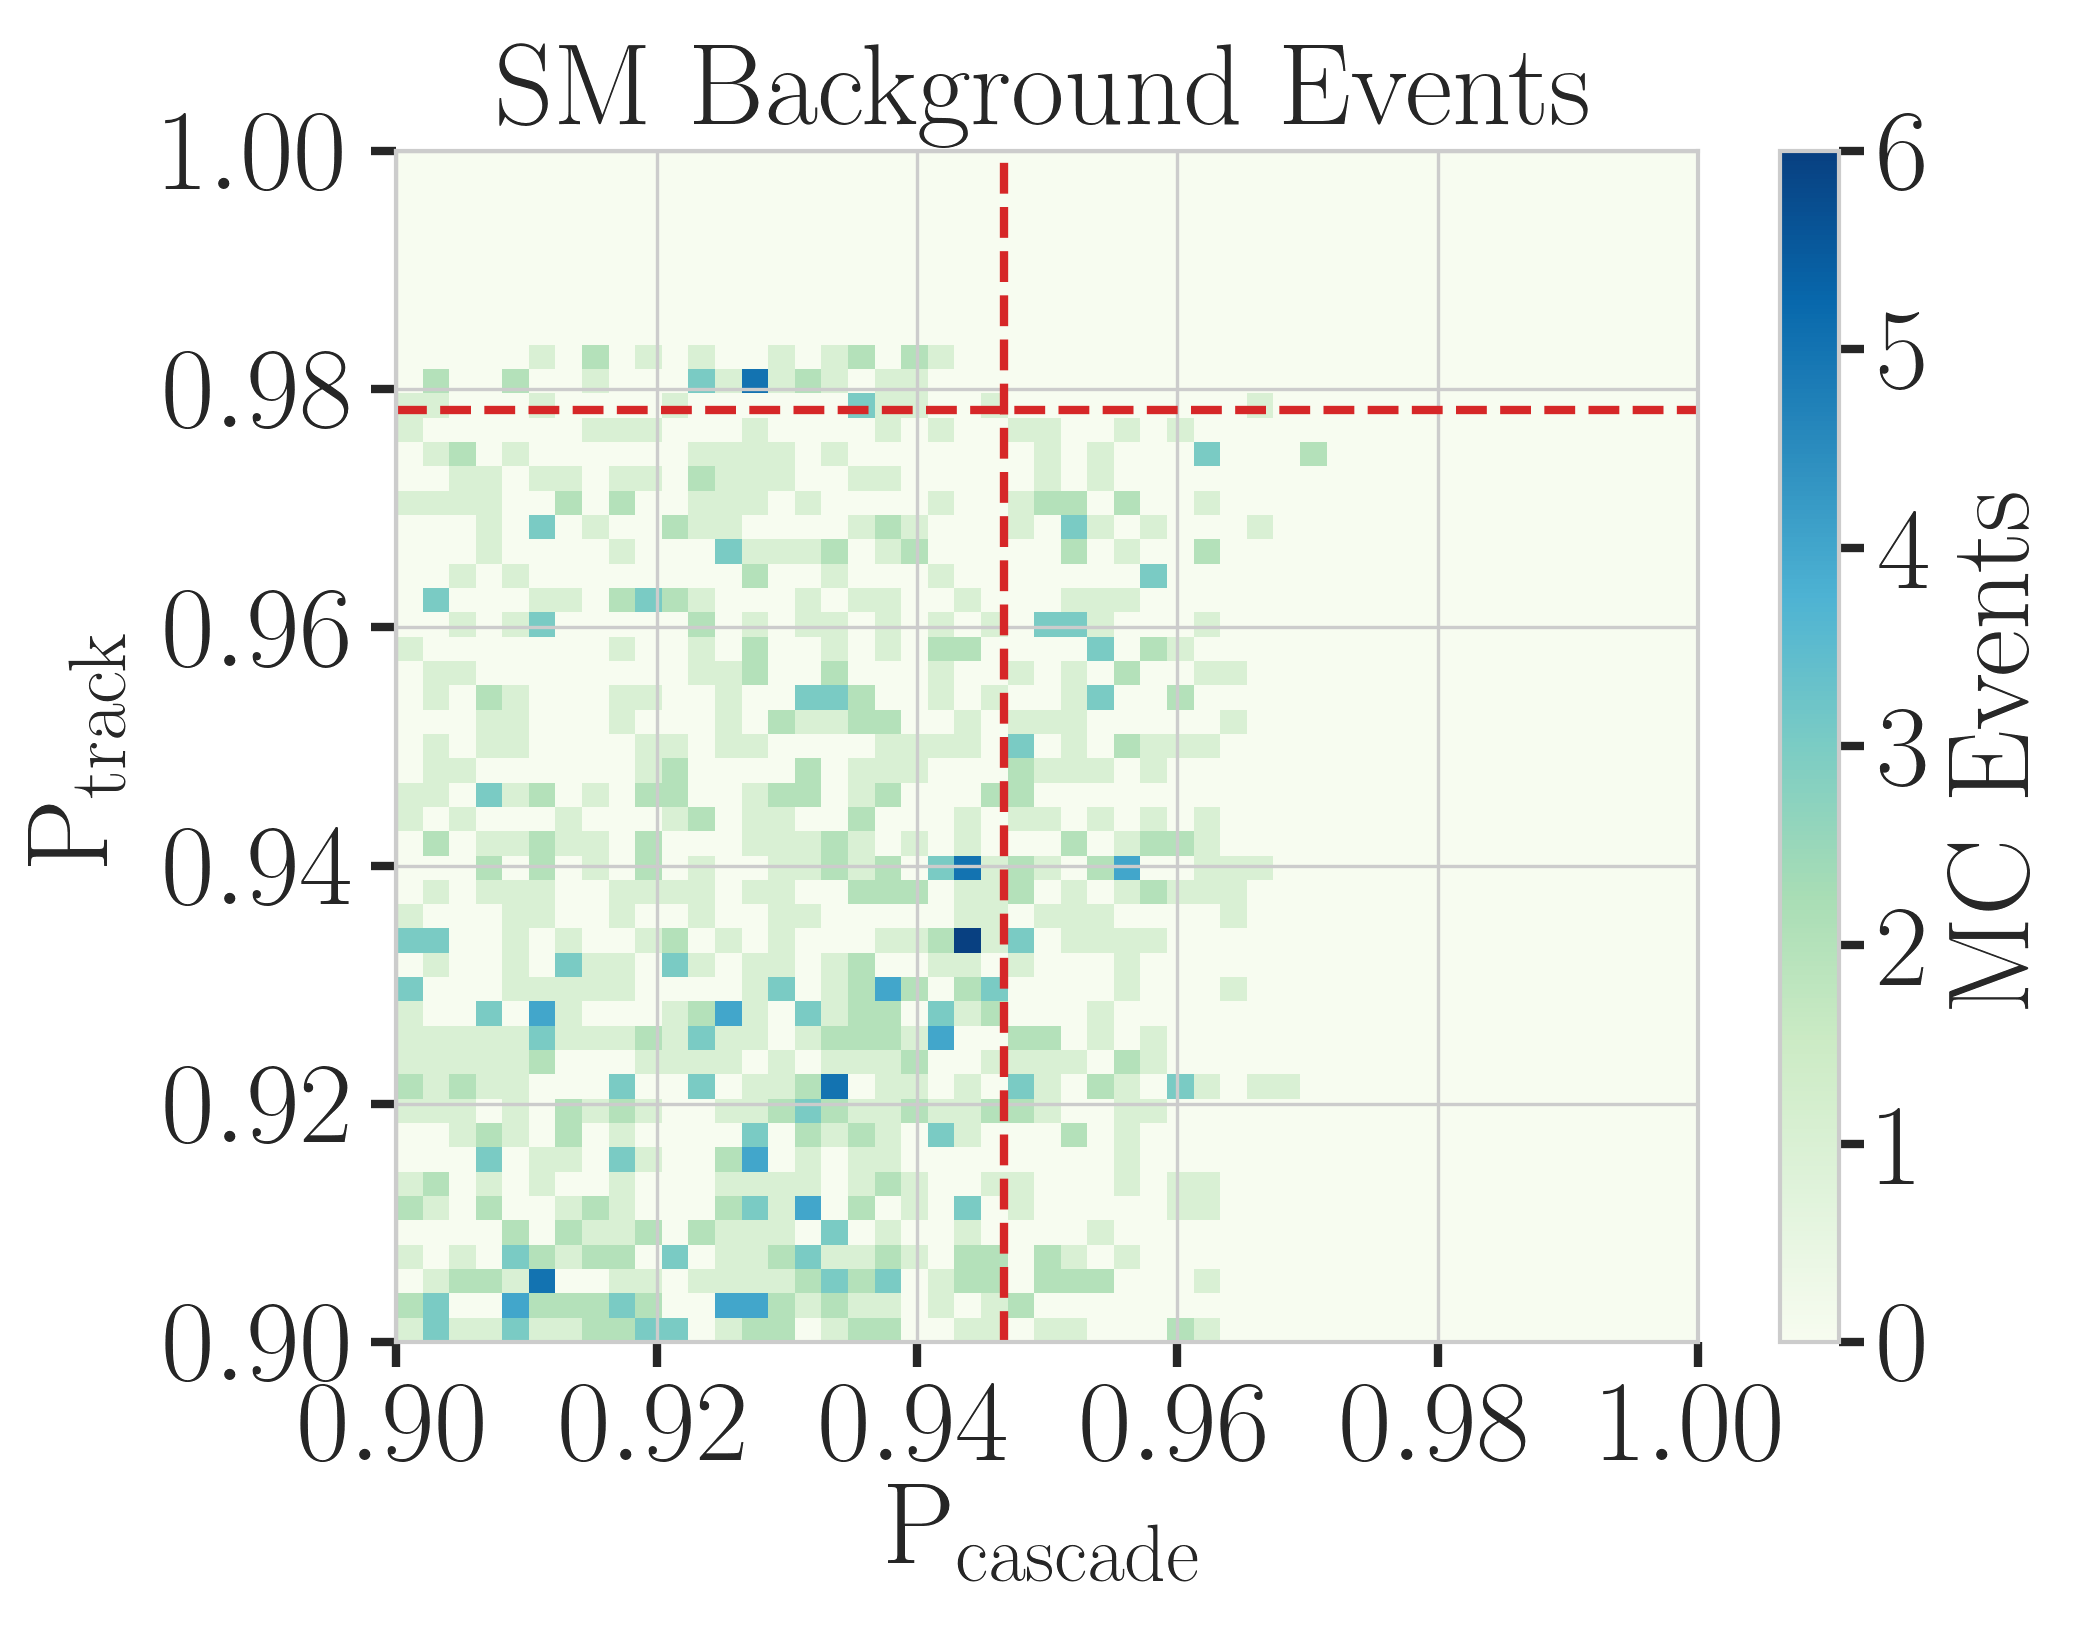
\includegraphics[width=0.49\linewidth]{figures/results/190607/classification/cascade_vs_track_class_prob_background_full_stats.png}
    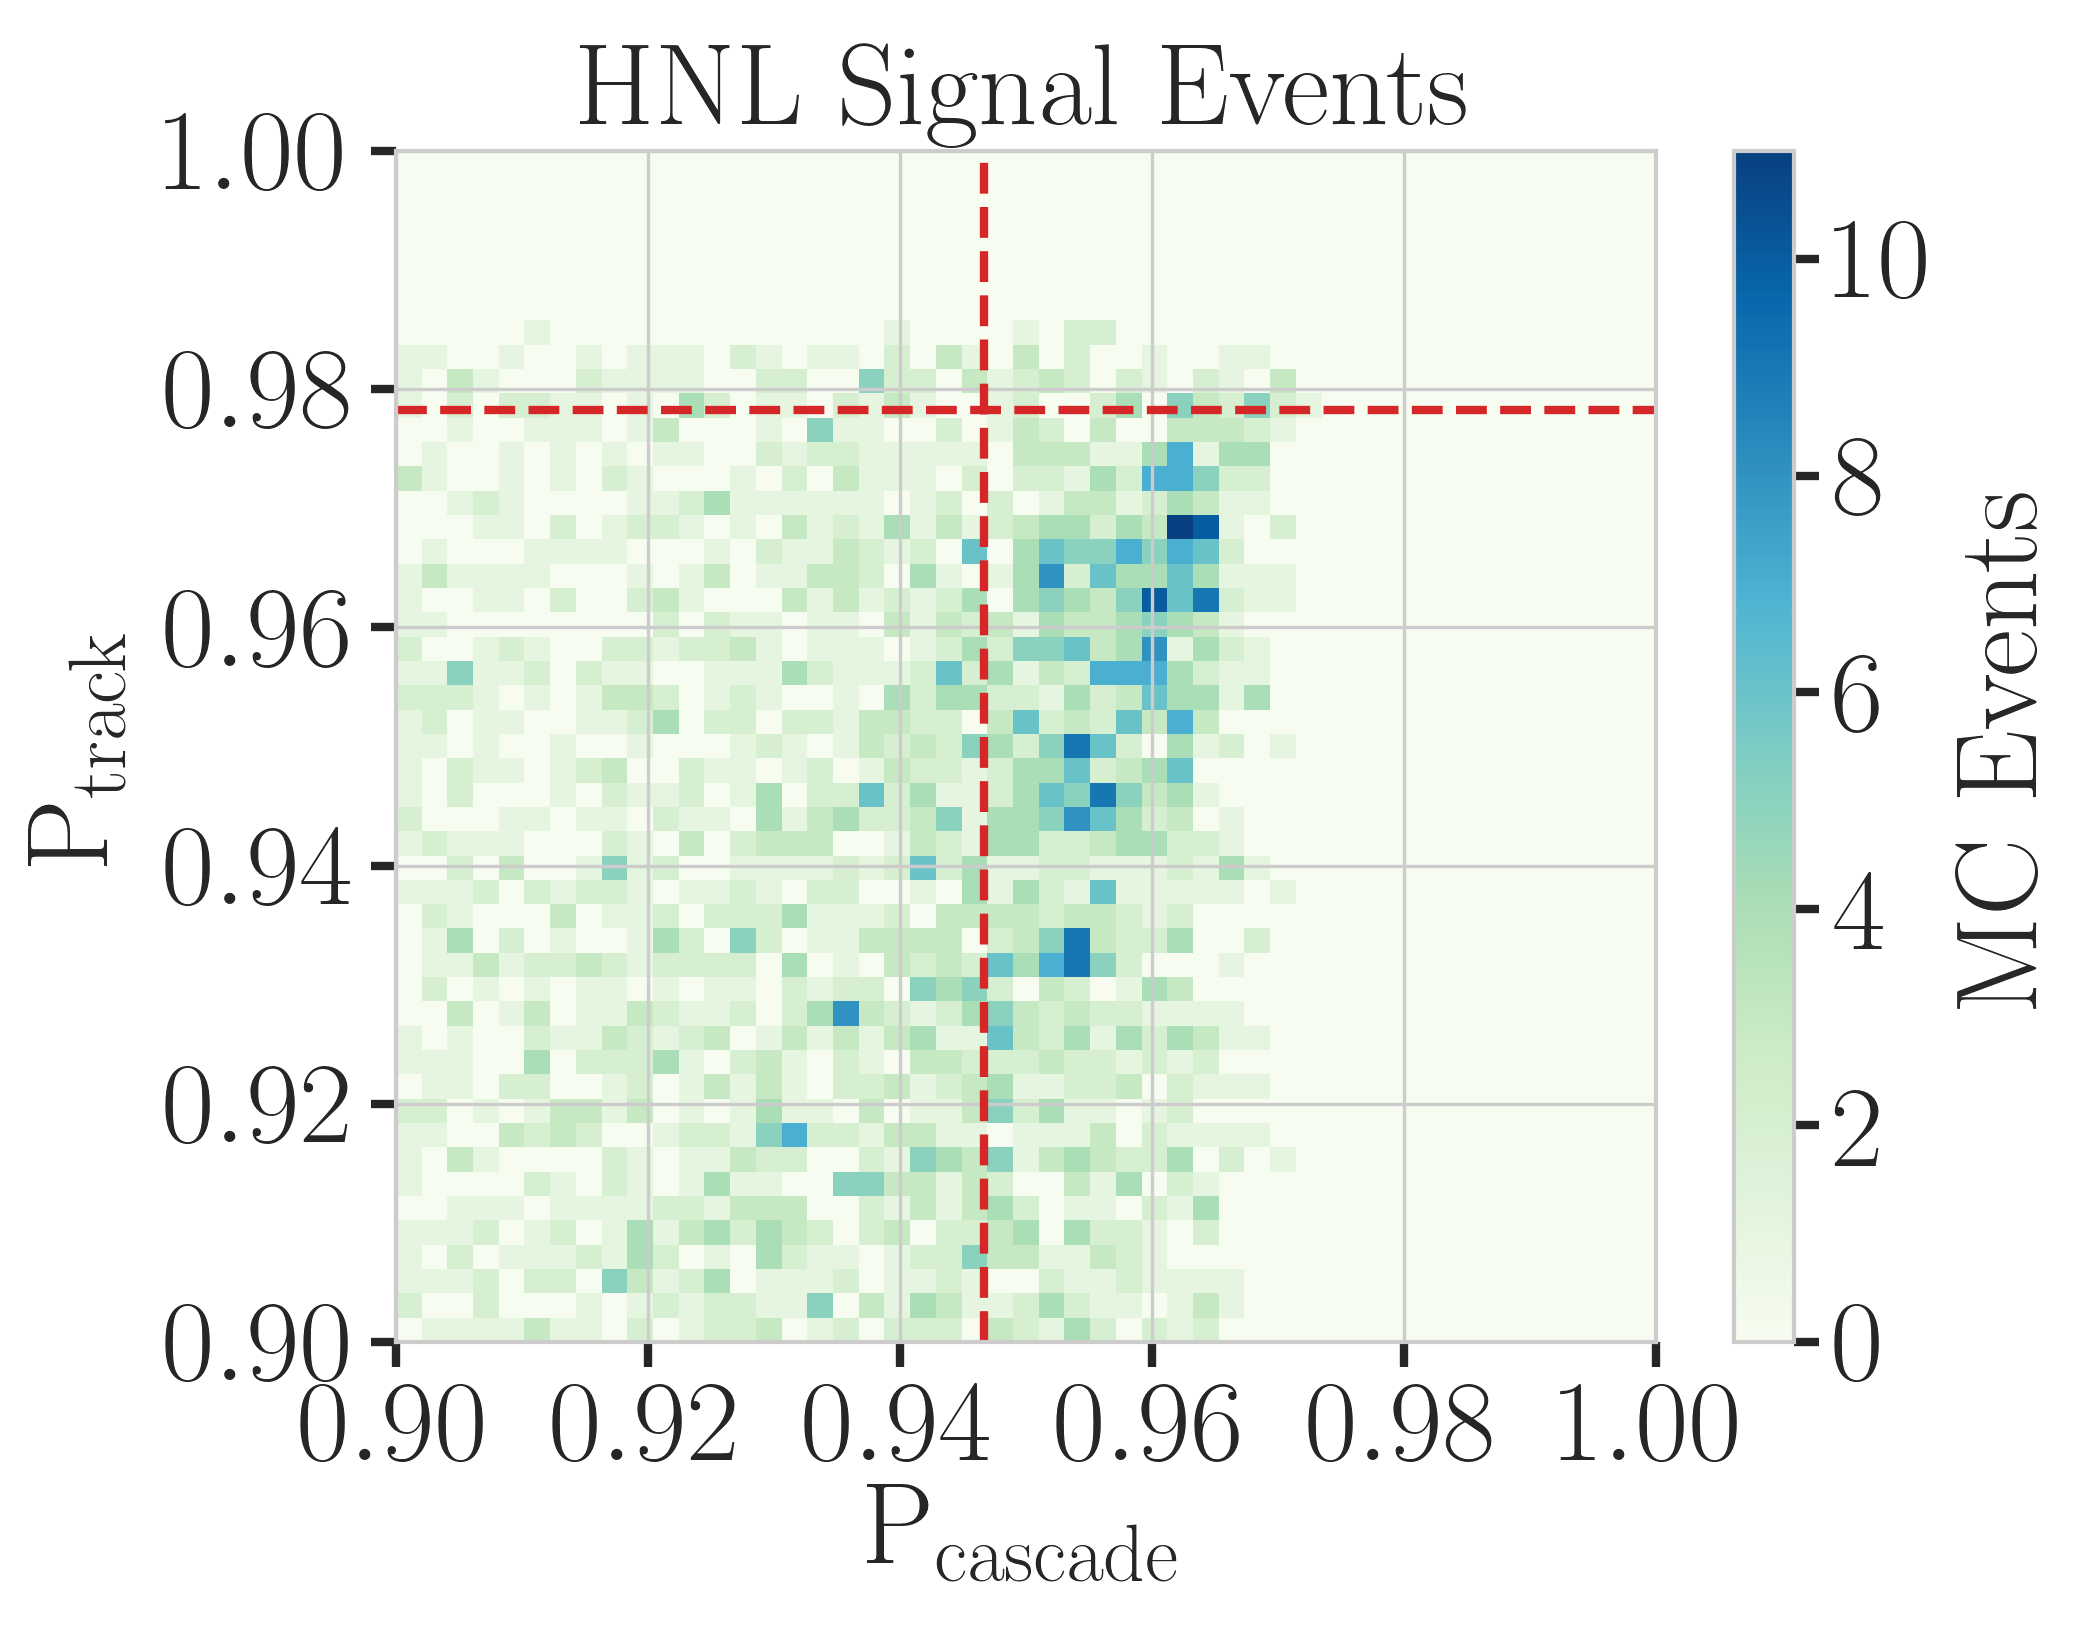
\includegraphics[width=0.49\linewidth]{figures/results/190607/classification/cascade_vs_track_class_prob_hnl_full_stats.png}
    \caption[Double-cascade classifier probabilities]{Output probabilities of the two classifiers trained to distinguish signal from track-like background and signal from cascade-like background. Shown are the MC event counts in the probability region close to 1, which means more signal like.}
    \labfig{two_classifier_selection}
\end{figure*}

By applying the two classifiers trained to distinguish signal from track and signal from cascade, it is possible to select a region with only signal events. This is visualized in \reffig{two_classifier_selection}, where the probabilities of 1 implies very signal like, and only the regions close to 1 are shown for both outputs, to highlight where a pure HNL sub-sample can be selected. When physical weights are applied to those signal events however, the expected event rate is very low, and even by assuming a highly optimistic mixing of 1, it would take more than \SI{20}{years} of data taking to observe a single event. Applying a weaker signal selection criterion will contain a large amount of background events, which dominate over the signal at $\sim2$ orders of magnitude for a mixing of $0.1$. With the current selection and reconstruction chain and a classical BDT, \textbf{it is not possible to distinguish double-cascade events from the SM background}.


\section{Analysis Reconstruction} \labsec{reconstruction}

An alternative method to search for HNLs is to look for an excess of single cascade-like events over the SM background, as will be described in more detail in \refch{analysis}. The reconstruction algorithm used for that purpose is a method that applies a \textit{convolutional neural network (CNN)}. It is both used to reconstruct the events properties and to determine some discriminating quantities. The latest muon neutrino disappearance result from IceCube~\sidecite{flercnn_analysis_result} is based on this reconstruction.


\subsection{Fast Low-Energy Reconstruction using Convolutional Neural Networks} \labsec{flercnn_reconstruction}

As the name \textit{Fast Low-Energy Reconstruction using Convolutional Neural Networks (FLERCNN)} already indicates, the FLERCNN reconstruction~\sidecite{Micallef:2022jvd, flercnn_proceedings}~\cite{flercnn} is a CNN optimized to reconstruct IceCube events at low energies ($<$\SI{100}{\gev}) in a fast and efficient manner, by leveraging the approximate translational invariance of event patterns within the detector. The architecture of the network is very similar to the preexisting IceCube CNN event reconstruction~\sidecite{dnn_reco_mirco}, but optimized on low-energy events and specifically tailored to include the DeepCore sub-array. Only the eight DeepCore strings and the central 19 IceCube strings are used for the reconstruction (compare to \reffig{icecube_top_view}). Because of the different z-positions of the DeepCore and IceCube DOMs, they are divided into two networks that are combined in the final layer of the network. The full architecture is shown in \reffig{flercnn_network_structure}. The first dimension of the network is the string index, while the second dimension is the order of the DOMs along the vertical axis. The horizontal position of the DOMs is not used, since the strings are arranged in an irregular pattern. The information from the DOM hits is summarized into five charge and time variables, which make up the last dimension of the input layer. The variables are the total summed charge, the time of the first hit, the charge weighted mean time of the hits, the time of the last hit, and the charge weighted standard deviation of the hit times.

\begin{figure}
    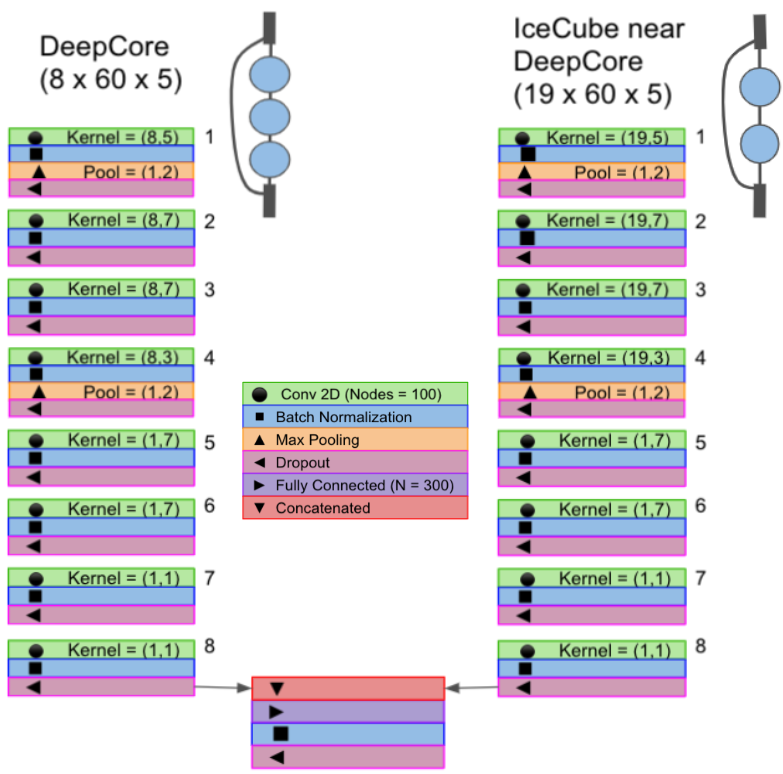
\includegraphics{figures/simulation_and_processing/flercnn/Detailed_CNN_Architecture_combined.png}
	\caption[FLERCNN architecture]{Architecture of the FLERCNN neural networks, taken from~\cite{flercnn_proceedings}.}
    \labfig{flercnn_network_structure}
\end{figure}

Five different networks are trained using this architecture. Three networks do the regression of the events' energy, cosine of the zenith angle, and the starting vertex ($x,y,z$ position), while two of them are used for classification. One is trained to predict the probability of the event being a $\nu_\mu$-CC event and the other to predict the probability of the event being an atmospheric muon. Each network is trained with a MC sample modified to have a flat distribution in the target variable, to be unbiased for that variable and ideally extending outside the target reconstruction region. For the classification tasks the loss function is the \textit{binary cross entropy} and the activation function is a \textit{sigmoid}. To perform the regression of zenith and vertex position, the loss function is the \textit{mean squared error (MSE)}, while for the energy it is the \textit{mean absolute percentage error}. The activation for all regression tasks is \textit{linear}.

\reffig{flercnn_resolution_example} shows the energy resolution of the FLERCNN reconstruction for muon neutrinos, compared to the performance of a classical, likelihood based reconstruction. It can be seen that the CNN based reconstruction is less biased and performs better up to $\sim$\SI{70}{\gev}. The resolution for electron neutrinos is shown in \refsec{flercnn_resolutions_appendix}.

\begin{figure}[h]
    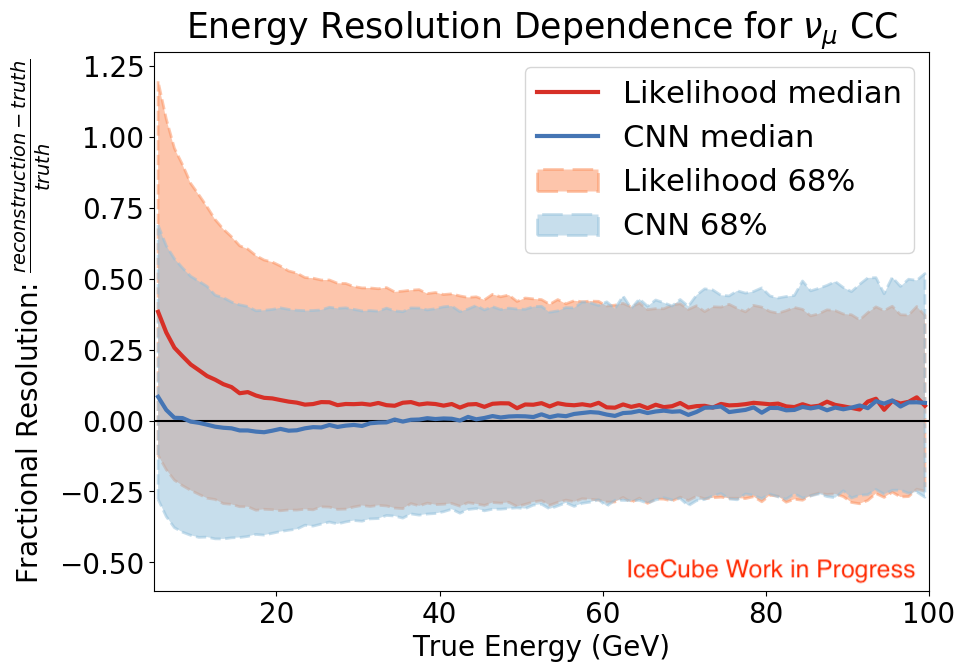
\includegraphics[width=0.8\textwidth]{figures/simulation_and_processing/flercnn/EnergyCNNResolution_NuMuCC_CompareLikelihoodReco.png}
	\caption[FLERCNN energy resolution for muon neutrinos]{Energy resolution of the FLERCNN reconstruction for muon neutrinos, compared to the performance of a classical, likelihood based reconstruction. Shown is the median fractional energy resolution and the \SI{68}{\percent} band as a function of the true energy.}
    \labfig{flercnn_resolution_example}
\end{figure}


\subsection{Analysis Selection} \labsec{analysis_cuts}

After the FLERCNN reconstruction is applied, a BDT classifier is used to further reduce the muon background for the final sample. The BDT is trained on five high level variables, where three are FLERCNN reconstruction variables (vertex $z$, $\rho_{36}$\sidenote{A radial variable that is often used in IceCube, is the horizontal distance to string 36 called $\rho_{36}$, which is basically the distance to the center of IceCube.}, and muon probability), and two are lower level variables (L4 muon classifier output and L5 corridor cut variable). To train the BDT, the FLERCNN nominal simulation set is used, only using events with $\cos(\theta)\leq 0.3$. The output of the BDT is the neutrino probability and a cut at 0.8 is applied to reject events with a high probability of being a muon. \reffig{muon_bdt_id} shows the output of the BDT classifier, where the neutrinos in both training and testing sets are gathered at 1 and muons are around 0, which shows great classification power. Since the probabilities for training and test sets are very similar, the BDT is not overtrained. The rate of neutrinos and muons as a function of the muon classifier probability threshold is shown in the right plot of \reffig{muon_bdt_id}, where it can be seen that at the chosen value of 0.8, the neutrino rate is two orders of magnitude above the muon rate.

\begin{figure*}
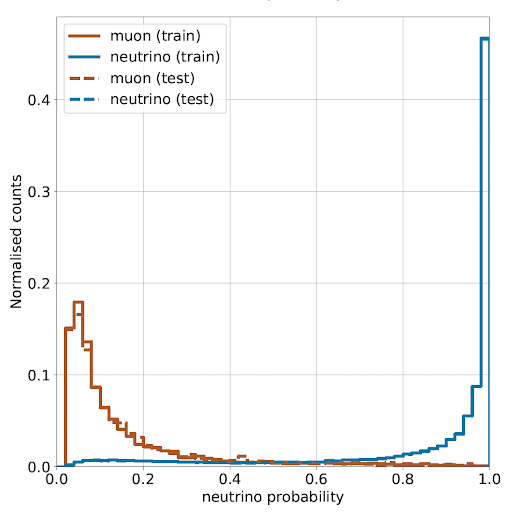
\includegraphics[width=0.44\linewidth]{figures/simulation_and_processing/flercnn/flercnn_muon_classifier.png}
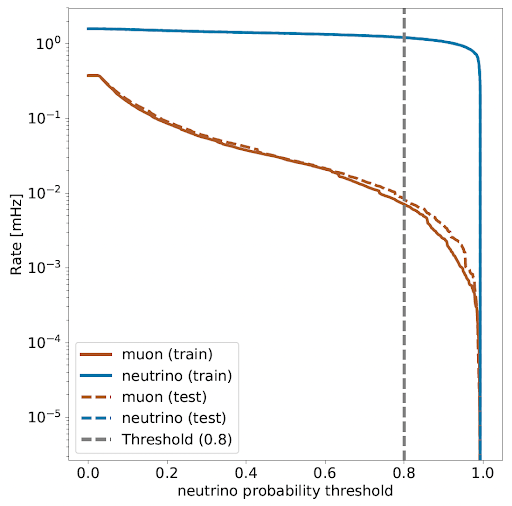
\includegraphics[width=0.44\linewidth]{figures/simulation_and_processing/flercnn/flercnn_muon_classifier_rate_vs_threshold.png}
\caption[FLERCNN muon classifier probability distributions]{FLERCNN muon classifier output score (left) and rate of neutrinos and muons as function of muon classifier cut (right).}
\labfig{muon_bdt_id}
\end{figure*}

To get the final, pure sample of well reconstructed neutrinos a final selection is applied. Parts of it are aiming to reject events with poor reconstruction quality, by requiring the events to fall into the DeepCore volume, where the denser, better instrumented detector leads to enhanced resolution. Conditions are applied on the vertex $z$ and $\rho_{36}$ and are listed in \reftab{analysis_cuts}. The FLERCNN reconstruction was optimized for atmospheric neutrino analyses which are mainly in the region below \SI{100}{\gev} and there are very few events with energies below \SI{5}{\gev}, so the reconstructed energy is required to be in that range. Additionally, rejecting events with fewer than seven hits in the selected DOMs used for FLERCNN showed to increase the resolution. The resulting final level rates and distributions for neutrinos and HNL will be presented in \refch{analysis}.

Parts of this selection are applied to make sure the agreement between data and MC is good. To remove coincident muon and neutrino events, the number of hits in the top 15 layers of IceCube DOMs and the number of hits in the outermost IceCube strings are required to be above 0.5 and 7.5, respectively. Coincident random noise events are removed by requiring more than three hit DOMs from direct photons\sidenote{\textit{Direct photons} are photons that were not scattered on their way from the interaction vertex to the DOM.}~\cite{low_energy_reco_IC}. Neither of the two coincident event types are simulated, which can be seen as bad agreement between data and MC. Lastly, the cosine of the reconstructed zenith angle is required to be smaller than 0.04 to reject down-going muons.

\begin{table}[h]
    \small
        \begin{tabular}{ lll }
        \hline\hline    
        \textbf{Variable} & \textbf{Threshold} & \textbf{Removed} \\     
        \hline\hline    
        Number of hit DOMs & $\geq 7$ & \SI{1.05}{\percent} \\
        Radial distance & < \SI{200}{\meter} & \SI{0.09}{\percent} \\
        Vertical position & \SI{-495}{\meter} < z < \SI{-225}{\meter} & \SI{5.48}{\percent} \\
        Energy & \SI{5}{\gev} < E < \SI{100}{\gev} & \SI{20.70}{\percent} \\    
        Cosine of zenith angle & < 0.04 & \SI{19.66}{\percent} \\
        Number of direct hits & > 2.5 & \SI{10.50}{\percent} \\
        Number of hits in top layers & < 0.5 & \SI{0.03}{\percent} \\
        Number of hits in outer layer & < 7.5 & \SI{0.001}{\percent} \\
        Muon classifier score & $\geq 0.8$ & \SI{23.90}{\percent} \\
        \hline
        \end{tabular}
    \caption[Final analysis selection criteria]{Selection criteria for the final analysis sample. They are partly aiming to increase the data/MC agreement, while others are rejecting events with poor reconstruction quality.}
    \labtab{analysis_cuts}
\end{table}
